%%%%%%%%%%%%%%%%%%%%%%%%%%%%%%%%%%%%%%%%%%%%%%%%%%%%%%%%%%%%%%%%%%%%%%%%%%%%%%%%%%%%%%%%%%%%%%%%%%%%%
% This template is distributed with ABSOLUTELY NO WARRANTY.
% It serves as a guideline and constitutes a basic structure for a
% thesis/dissertation. The user assumes full responsibility for formatting
% and typesetting their document and for verifying that all the thesis
% requirements set by the University of Tennessee are met. Please refer to the most
% recent UT thesis guide (http://gradschool.utk.edu/thesesdissertations/formatting/)
% or contact the thesis consultant (http://gradschool.utk.edu/thesesdissertations/).
% Please report any bugs to the thesis consultant.
%%%%%%%%%%%%%%%%%%%%%%%%%%%%%%%%%%%%%%%%%%%%%%%%%%%%%%%%%%%%%%%%%%%%%%%%%%%%%%%%%%%%%%%%%%%%%%%%%%%%%
% O P T I O N S:
% 1. thesis/dissertation
% 2. monochrome
% 3. all options provided by the report class
%%%%%%%%%%%%%%%%%%%%%%%%%%%%%%%%%%%%%%%%%%%%%%%%%%%%%%%%%%%%%%%%%%%%%%%%%%%%%%%%%%%%%%%%%%%%%%%%%%%%%
%First, is this a thesis or dissertation? Choose one by commenting out the one you don't need:
\documentclass[thesis,letterpaper,12pt]{utthesis} % thesis
%\documentclass[dissertation,letterpaper,12pt]{utthesis} %dissertation
% some alternatives are:
%\documentclass[thesis,monochrome,letterpaper,12pt]{utthesis} %thesis, monochrome text
\renewcommand{\baselinestretch}{1.5} 	 % line Spacing
%%%%%%%%%%%%%%%%%%%%%%%%%%%%%%%%%%%%%%%%%%%%%%%%%%%%%%%%%%%%%%%%%%%%%%%%%%%%%%%%%%%%%%%%%%%%%%%%%%%%%
% TO DO: FILL IN YOUR INFORMATION BELOW - READ THIS SECTION CAREFULLY
%%%%%%%%%%%%%%%%%%%%%%%%%%%%%%%%%%%%%%%%%%%%%%%%%%%%%%%%%%%%%%%%%%%%%%%%%%%%%%%%%%%%%%%%%%%%%%%%%%%%%
\title{Implementation of Multi-phase Species Transport into VERA-CS for Molten Salt Reactor Analysis}	       	% title of thesis/dissertation
\author{Robert Zachary Taylor}                			% author's name
\copyrightYear{2019}            				% copyright year of your thesis/dissertation
\graduationMonth{May}           				% month of graduation for your thesis/dissertation
\degree{Master of Science}	    			% degree: Doctor of Philosophy, Master of Science, Master of Engineering...
\university{The University  of Tennessee, Knoxville}	% school name
%%%%%%%%%%%%%%%%%%%%%%%%%%%%%%%%%%%%%%%%%%%%%%%%%%%%%%%%%%%%%%%%%%%%%%%%%%%%%%%%%%%%%%%%%%%%%%%%%%%%%
% LOAD SOME USEFUL PACKAGES. 
% No need to change anything here, although if you'd like to add packages you can do that here. Note that packages preloaded with the utthesis class are: amsmath,amsthm,amssymb,setspace,geometry,hyperref,and color
%%%%%%%%%%%%%%%%%%%%%%%%%%%%%%%%%%%%%%%%%%%%%%%%%%%%%%%%%%%%%%%%%%%%%%%%%%%%%%%%%%%%%%%%%%%%%%%%%%%%%
\usepackage{nomencl}                    % produces a nomenclature
\usepackage{float}                      % figure floats
\usepackage[numbers]{natbib}                     % this package allows you to link your references
\usepackage{graphicx}					% graphics package
\graphicspath{ {figures/}{figures/eps/}{figures/pdf/} }% specify the path where figures are located
\usepackage{fancyhdr}                   % fancy headers and footers
\usepackage{url}                        % nicely format url breaks
\usepackage[inactive]{srcltx}		 	% necessary to use forward and inverse searching in DVI
\usepackage{relsize}                    % font sizing hierarchy
\usepackage{booktabs}                   % professional looking tables
\usepackage[config, labelfont={bf}]{caption,subfig} % nice sub figures
\usepackage{mathrsfs}                   % additional math scripts
\usepackage[titletoc]{appendix}			% format appendix correctly
\usepackage{pdflscape}					% to produce landscape pages if necessary
\usepackage{threeparttable}		% used to add footnote to bottom of table
\usepackage{textcomp}
\usepackage{rotating}
\usepackage{enumitem}
\usepackage{placeins}

%%%%%%%%%%%%%%%%%%%%%%%%%%%%%%%%%%%%%%%%%%%%%%%%%%%%%%%%%%%%%%%%%%%%%%%%%%%%%%%%%%%%%%%%%%%%%%%%%%%%%%
% This section formats landscape pages properly with the correct page number.
% This code is only necessary when landscape pages are needed and can be left alone
%%%%%%%%%%%%%%%%%%%%%%%%%%%%%%%%%%%%%%%%%%%%%%%%%%%%%%%%%%%%%%%%%%%%%%%%%%%%%%%%%%%%%%%%%%%%%%%%%%%%%%

\fancypagestyle{mylandscape}{
	\fancyhf{} %Clears the header/footer
	\fancyfoot{% Footer
    \makebox[\textwidth][r]{% Right
      \rlap{\hspace{.75cm}% Push out of margin by \footskip
        \smash{% Remove vertical height
          \raisebox{4.87in}{% Raise vertically
            \rotatebox{90}{\thepage}}}}}}% Rotate counter-clockwise
  \renewcommand{\headrulewidth}{0pt}% No header rule
  \renewcommand{\footrulewidth}{0pt}% No footer rule
}


%%%%%%%%%%%%%%%%%%%%%%%%%%%%%%%%%%%%%%%%%%%%%%%%%%%%%%%%%%%%%%%%%%%%%%%%%%%%%%%%%%%%%%%%%%%%%%%%%%%%%
\begin{document}
    \pagenumbering{alph} % this is needed to clear certain issues with the hyperref package
    %
    \addToPDFBookmarks{0}{Front Matter}{rootNode} % create a root node named "Front Matter" in the pdf bookmarks
    \addToPDFBookmarks{1}{Title}{a} % add a pdf bookmark to the title page
    \makeTitlePage % make the title page.
    %
    \pagenumbering{roman}
    \setcounter{page}{2}
    %
    \makeCopyrightPage % make the copyright page
    %
%%%%%%%%%%%%%%%%%%%%%%%%%%%%%%%%%%%%%%%%%%%%%%%%%%%%%%%%%%%%%%%%%%%%%%%%%%%%%%%%%%%%%%%%%%%%%%%%%%%%%
%The dedication and acknowledgments are optional. If you wish not to include them, simply comment out both the "\addToPDF..." line and the "\include{...}" line for each.
%%%%%%%%%%%%%%%%%%%%%%%%%%%%%%%%%%%%%%%%%%%%%%%%%%%%%%%%%%%%%%%%%%%%%%%%%%%%%%%%%%%%%%%%%%%%%%%%%%%%%
    \addToPDFBookmarks{1}{Dedication}{b} % add a pdf bookmark to the dedication page
    \chapter*{}
\begin{center}
{\centering \it Dedicated to all the round pegs in the square holes}
\end{center}  % include the dedication

    \addToPDFBookmarks{1}{Acknowledgments}{c} % add a pdf bookmark to the acknowledgments page
    \chapter*{Acknowledgments}
I would like to thank Ivan Maldonado, Ben Collins and Bob Salko for their mentorship and support. This report was funded by the US Department of Energy's Molten Salt Reactor Campaign headed by Lou Qualls.  % include the acknowledgments
    
    \addToPDFBookmarks{1}{Abstract}{e} % add a pdf bookmark to the abstract page
    \chapter*{Abstract}\label{ch:abstract}
Molten salt reactors (MSRs) are a class of next generation nuclear reactors that have received recent industrial and research interest. In this manuscript, a generalized multi-phase species transport solver was derived and implemented into the Virtual Environment for Reactor Applications (VERA) computing suite, with the purpose to extend this tool to analyze liquid fueled MSRs, in which fission products (FPs) are generated and transported throughout the primary system. 

In order to test the accurate functionality of species transport, a number of simplified test problems were developed. These "unit tests" are meant to demonstrate the capability and accuracy of the utilized solution methods. Of the FPs discussed, xenon is of particular interest and impact to reactor operation. The steady-state and transient distribution of ${}^{135}$Xe is analyzed in many of the unit tests. Finally, a simplified test case of the Molten Salt Reactor Experiment (MSRE) is analyzed to demonstrate the systematic effects of boundary conditions and solution parameters. The goal of this thesis is to derive and implement a set of equations which will accurately model the spatial distribution of FPs in MSRs. % your abstract

    \addToPDFBookmarks{0}{Table of Contents}{f}
    \tableofcontents % generate a table of contents
    \listoftables % generate a list of tables
    \listoffigures % generate a list of figures
   
    \newpage
    \pagenumbering{arabic}
    \setcounter{page}{1}
    %%%%%%%%%%%%%%%%%%%%%%%%%%%%%%%%%%%%%%%%%%%%%%%%%%%%%%%%%%%%%%%%%%%%%%%%%%%%%%%%%%%%%%%%%%%%%%%%%%%%%
    % INCLUDE THE CHAPTERS STARTING WITH THE NOMENCLATURE IF PRESENT
    %%%%%%%%%%%%%%%%%%%%%%%%%%%%%%%%%%%%%%%%%%%%%%%%%%%%%%%%%%%%%%%%%%%%%%%%%%%%%%%%%%%%%%%%%%%%%%%%%%%%%
    \include{front-matter}
    \chapter{Introduction} \label{ch:introduction}

Recent commercial interest in molten salt reactors (MSRs) creates the need for a deep understanding of fission product behavior. Some of the major features that make MSRs so appealing include simplified; fuel cycle, fuel handling, and waste disposal, as well as other versatility and economic benefits \cite{williams1996}. Historically, the only molten salt reactor to ever operate at power was the molten salt reactor experiment experiment (MSRE), an 8-MW(th) nuclear reactor that was operated at the Oak Ridge Nation Laboratory (ORNL) from 1965-1969. The goal of the MSRE was to demonstrate the technical validity of such a reactor at a time when the global supply of uranium was still unknown. This reactor was successfully operated using both ${}^{235}U$ and ${}^{233}U$ \cite{engel1970}. Throughout history, many attempts have been made in order to model the physical and chemical behavior of MSRs. These include many historical reports from the MSRE days on chemistry \cite{grimes1970}, \cite{baes1965}, \cite{cantor1968}, nuclear interactions \cite{nestor1960}, \cite{bell1970}, \cite{prince1962} and mass transport \cite{engel1971}, \cite{peebles1968}, \cite{kedl1967}, \cite{kedl1972}, to name a few. There have also been more recent reports on each of these subjects in the following references: \cite{cammi2011}, \cite{benes2008}, \cite{eades2016}, \cite{wu2017} and \cite{zack2018}. Many of these reports discuss either theory or application in a modeling and simulation framework. The purpose of this thesis is to present a fundamental background on chemical species transport, fission product behavior for a liquid fueled system and implementation of species transport into the Virtual Environment for Reactor Analysis (VERA) for its extension to MSRs (VERA-MSR). Implementation of the generalized species transport solver was accomplished by Dr. Robert Salko and tested by both the author and Dr. Salko \cite{zack2018}. In addition to the generalized species transport, a new multi-phase gas sparging model has been implemented by the author for the analysis of fission product gas removal. 



\section{Nuclear Energy}
Commercial nuclear reactors work on the basis of sustained fission reactions. Nuclear fission is the process whereby an atomic nucleus is split into smaller fragments by the capture of a neutron. These smaller fragments are known as fission products (FPs). The combined mass of the smaller fragments is less than the mass of the original nucleus, and so the missing mass, or "mass defect," is converted into energy using Einstein's famous Equation \ref{eq:Einstein}

\begin{equation}
    \Delta E = \Delta m C^{2}
    \label{eq:Einstein}
\end{equation}

Commercial reactors primarily work with uranium, within which the ${}^{235}U$ isotope is fissile. However, elements such as plutonium and thorium have also been used in power reactors. For ${}^{235}U$ a neutron induced fission reaction is shown in Equation \ref{eq:nuclearFission} \cite{duderstadt1976}.

\begin{equation}
    {}^{235}_{92}U + {}^{1}_{0}n \rightarrow {}^{236}_{92}U^{*} \rightarrow \text{Fission products} + \text{neutrons} + \text{energy}
    \label{eq:nuclearFission}
\end{equation}

About 200 MeV of energy is released from each fission event along with typically two fission fragments and approximately two or three neutrons. Energy release from fission is characterized by the following contributions \cite{fissionBasics}:

\begin{itemize}[label={}]
    \item Kinetic energy of fission products $\approx$ 165 MeV (83\%) 
    \item Gamma rays $\approx$ 7 MeV (4\%)
    \item Kinetic energy of the neutrons $\approx$ 6 MeV (3\%) 
    \item Energy from fission product beta-decay $\approx$ 7 MeV (4\%) 
    \item Gamma rays from fission products $\approx$ 6 MeV (3\%)
    \item Neutrinos from fission products $\approx$ 9 MeV (5\%) 
\end{itemize}

Once fission reactions and neutron populations reach a steady state at a target power level, they are maintained at a constant level so that the rate of fission events and neutrons in a previous generation equal those in the next generation, which characterizes a self-sustaining chain reaction and a "critical" system. If the rate of neutrons generated from the previous generations is increasing, the reaction is said to be "supercritical." Alternatively, if this rate is decreasing, the reaction is said to be "subcritical." Controlling the neutron balance in nuclear reactors is done by balancing the production of neutrons from fission and neutron-producing FPs against the losses due to leakage and absorption of neutrons. Absorbing materials can be removable, such as control blades, or static such as burnable absorbers that are fabricated into the fuel elements, or reactor structural materials.  Leakage is controlled by the geometrical arrangement of fuel and moderating materials and is related to the curvature or gradients of the neutron flux distribution, whereby larger reactors generally have flatter power distributions and lower leakage than smaller reactors.  Neutrons born from fission, approximately 2 to 3 from each fission, can have a wide range of energy values, although they're preferentially born at about 1 to 2 MeV.  In U-235 fueled reactors, neutrons of lower energy have a higher probability of inducing fission, therefore, neutron moderators are commonly employed to slow down the neutrons to thermal energies (below 1 eV), thus allowing more fission events to occur.  The rate at which fission events occur will be discussed later in the manuscript.  

\section{Molten Salt Reactors}
MSRs have two common designs; one in which fissile material held in place like traditional nuclear reactors. In this design, the molten salt simply acts as a heat transfer fluid, carrying the heat away from the fuel elements. The other and more popular design dissolves the fissile material into the circulating salt, thus allowing for fission products to disperse around the primary loop.  This greatly differs from traditional light water reactors (LWRs) where fissile material is maintained in a fixed solid form. Fissile material in MSRs is dissolved in either a chloride or fluoride based salt and is often referred to as the solvent or carrier salt. Fluoride salts are generally used in applications where the reactor operates with neutrons preferentially in the thermal energy spectrum, whereby chloride salts favor the fast energy range.

MSRs produce the unique challenge of allowing fission products to flow throughout the system. Fission products exist in multiple phases (gas, liquid, solid) with each phase interacting with various process equipment contained in the flow loop \cite{grimes1975}. In order to accurately model a dynamic and steady-state fission product behavior, all three phase fields must be resolved.  

This report focuses on three general categories of fission products:

\begin{itemize}
	\item Salt seekers
	\item Noble metals
	\item Noble gases
\end{itemize}

Salt seekers are fission products that will form stable ionic compounds with the carrier salt of interest (XF,XCl) where X is the fission products. Noble metals are fission products which will undergo redox reactions in solution to form solid elemental metals which can plate out in the system. Noble gases are fission products which will be in the gaseous state which are slightly soluble in the carrier salt. These FPs will be processed in an off-gas system \cite{grimes1975}.  

Volatile fission products are a subclass of fission products that can include fission products from both noble metals and gases. These are known as volatile because they do not form stable ionic compounds with the carrier salt. This class of FPs have a noticeable impact on system behavior and cannot be ignored. These impacts include but not limited to: depositing on process equipment, affecting neutron economy, forming collides and other undesired compounds. 


\subsection{Molten Salt Reactor Experiment}
The MSRE was an experiment conducted in the 1960s at ORNL to deduce the validity of molten salt reactors. This was a fluid fueled 8-MW thermal nuclear reactor. During operation, molten salt is continuously circulated about a primary loop containing: the reactor vessel, fuel pump, and heat exchanger. This primary loop contained molten salt with the composition described in Table \ref{tab:MSRE_salt} \cite{engel1970} and a depiction of the process flow diagram is shown in Figure \ref{fig:MSRE_flow_diagram}. 


Salt enters the reactor vessel through orifices at the top portion of the reactor. The holes impart a spiraling flow which moves down the sides of the reactor and up through the bottom head. Salt then flows up the moderator channel tubes shown in Figure \ref{fig:MSRE_fuel_chan}. While the fuel salt is flowing up the channels, graphite moderates the neutrons, inducing fission and power generation. Upon exiting the core, the molten salt then enters the pump bowl shown in Figure \ref{fig:MSRE_pump}. 

Salt enters the fuel pump via the suction port at the bottom of the pump. The pump bowl had two main functions, sample collection and off noble gas removal. The pump bowl had a head space which was constantly purged using a cover gas. Upon discharge, a portion of salt was redirected back into the head space of the pump bowl. This salt was forced through a perforated ring which allowed gas to be removed from the salt via the cover gas. After discharge, the salt flows through a heat exchanger which exits back into the reactor vessel and the process is repeated \cite{engel1970}.

\vspace{12.7mm} %5mm vertical space

\begin{table}[htbp!]
   \caption{\label{tab:MSRE_salt} MSRE operation materials}
   \centering
   \begin{tabular}{l llllllllll}
   \hline
   Fuel Salt & ${}^{7}LiF$-$BeF_{2}$-$ZrF_{4}$-$UF_{4}$ (65.0-29.1-5.0-0.9 mole\%) \\ [1ex]
   Coolant Salt & ${}^{7}LiF$-$BeF_{2}$ (66-34 mole\%) \\ [1ex]
   Moderator & Grade CGB graphite \\ [1ex]
   Salt Containers & Hastelloy-N (68-Ni, 17-Mo, 7-Cr, 5-Fe weight \%) \\ [1ex]
   Cover Gas & Helium/Argon \\ [1ex]
   \hline
   \end{tabular}
\end{table}

\newpage

\vspace{12.7mm} %5mm vertical space

\begin{figure}[p]
  \centering
  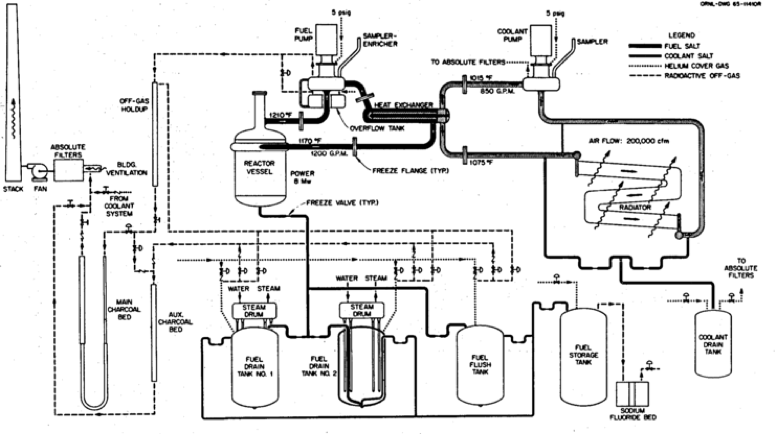
\includegraphics[width=5in]{images/MSRE_flow_diagram.png}\\
  \caption{MSRE process flow diagram}
  \label{fig:MSRE_flow_diagram}
\end{figure} 

\newpage

\begin{figure}[p]
  \centering
  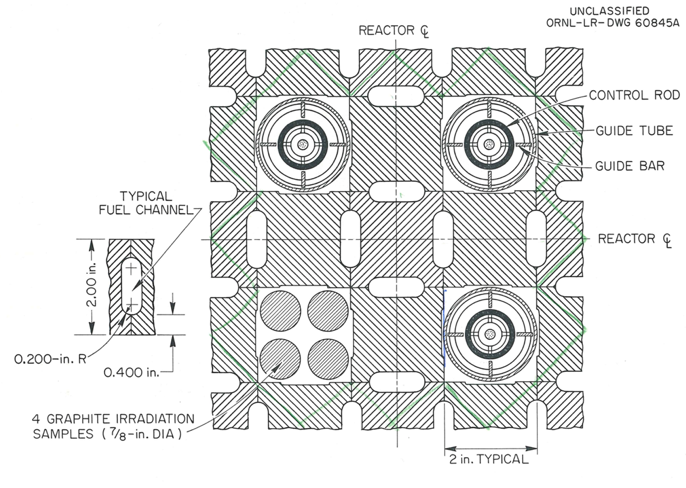
\includegraphics[width=4in]{images/MSRE_fuel_channel.png}\\
  \caption{MSRE graphite fuel channels}
  \label{fig:MSRE_fuel_chan}
\end{figure} 

\vspace{12.7mm} %5mm vertical space

\begin{figure}[p]
  \centering
  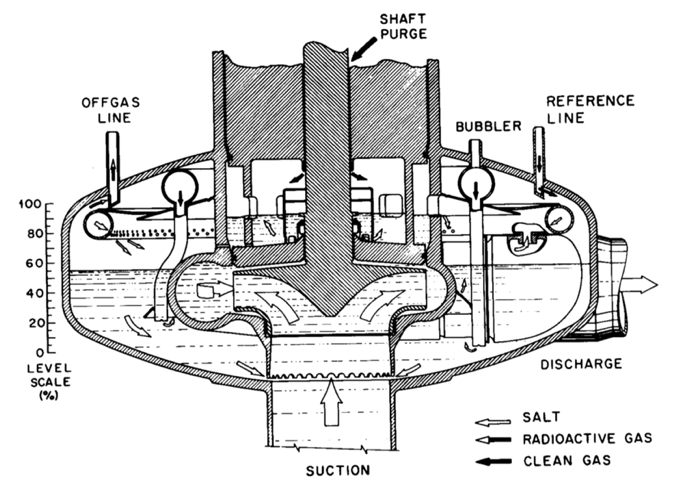
\includegraphics[width=4in]{images/MSRE_pump.png}\\
  \caption{MSRE pump}
  \label{fig:MSRE_pump}
\end{figure} 

\FloatBarrier
\newpage

% Fission produdcts
\subsection{Fission Product Elements}
Although it is possible to generate most of the elements on the Periodic Table, this report will only focus on a portion of fission products which are known to be volatile. Table \ref{tab:common_fission_products} shows common fission products in their respective categories based on MSRE experience \cite{grimes1975}. Elements that have been removed in previous simulation efforts are listed in Table \ref{tab:common_fission_products_removed} \cite{powers2016}. A visual representation of elemental grouping on the periodic table is shown in Figure \ref{fig:periodic_table_fp}. In general, the nuclear reaction for a given fissionable isotope show in equation

% fission equation
\begin{align}
	\ YX_{4} + n  \rightarrow 2FP + 4X^{-}  + \text{neutrons} + \text{energy}
	& \label{eq:fission_reaction}
\end{align}

Where Y is the fissionable isotope, X is the salt of interest (Cl or F) and FP are the fission products produced.

\subsubsection{Salt Seekers}
Salt seekers form stable fluoride or chloride compounds which are soluble in the carrier salt. These compounds are almost completely found in the molten fuel \cite{grimes1970}. Stability of salt seekers is approximated by energy of formation. Compounds that have a more negative energy of formation will be more stable than those same elements forming other compounds with higher heats of formation. Many of the salt seeker fission products are rare earth elements with high neutron capture cross sections \cite{baes1974}. Neutron economy can be increased if these elements are separated from the reaction medium.  

\subsubsection{Noble Metals}
Noble metals are born as ions from fission and decay of their precursors. They are unstable in the fuel salt and do not live as ions for very long. Once they are born they quickly undergo reduction reactions and are homogeneously dispersed in the salt. This group of fission products tend to deposit on surfaces inside the flow loop, which can include: heat exchanger, pipes, reactor vessel and moderator. Noble metals also deposit on liquid-gas interfaces such as bubble surfaces and display some properties of surface active agents \cite{kedl1972}. 

\newpage

% Table of common fission products
\begin{table}[p]
   \caption{\label{tab:common_fission_products} Common fission products}
   \centering
   \begin{threeparttable}
   \begin{tabular}{l llllllllll}
   \hline
   \textbf{Group} & \textbf{Element}\\
   \hline 
   Salt seekers & Rb, Sc, Sr, Ba, Y, Zr, Lanthanides \\ [1ex]
   Noble metals & $Nb^{a}$, Mo, Tc, Ru, Rh, Pb, Ag, Sb, $Te^{b}$, $I^{b}$ \\ [1ex]
   Noble gases & Xe, Kr \\ [1ex]
   \hline
   \end{tabular}
   \begin{tablenotes}\footnotesize
   \item[a] Niobium is borderline and depends on redox condition of the salt 
   \item[b] Iodine can form iodides and remain in the slat however it is included because of its tellurium predecessor \cite{grimes1975}
   \end{tablenotes}
   \end{threeparttable}
\end{table}


\vspace{12.7mm} %5mm vertical space

% table of fissions products that people want to remove
\begin{table}[p]
   \caption{\label{tab:common_fission_products_removed} Common fission products removed from salt}
   \centering
   \begin{tabular}{l llllllllll}
   \hline
   \textbf{Group} & \textbf{Element}\\
   \hline 
   Volatile gases & Xe, Kr \\ [1ex]
   Noble metals & Se, Nb, Mo, Tc, Ru, Rh, Pb, Ag, Sb, Te \\ [1ex]
   Seminoble metals & Zr, Cd, In, Sn \\ [1ex]
   Volatile fluorides & Br, I \\ [1ex]
   Rate earth elements & Y, La, Ce, Pr, Nd, Pm, Sm, Gd, Eu \\ [1ex]
   Discard & Rb, Sr, Cs, Ba \\ [1ex]
   \hline
   \end{tabular}
\end{table}

\FloatBarrier

\newpage

% periodic table figure. Need to find source for actual table picture. Or find a new picture and redo the coloring
\begin{figure}[p]
  \centering
  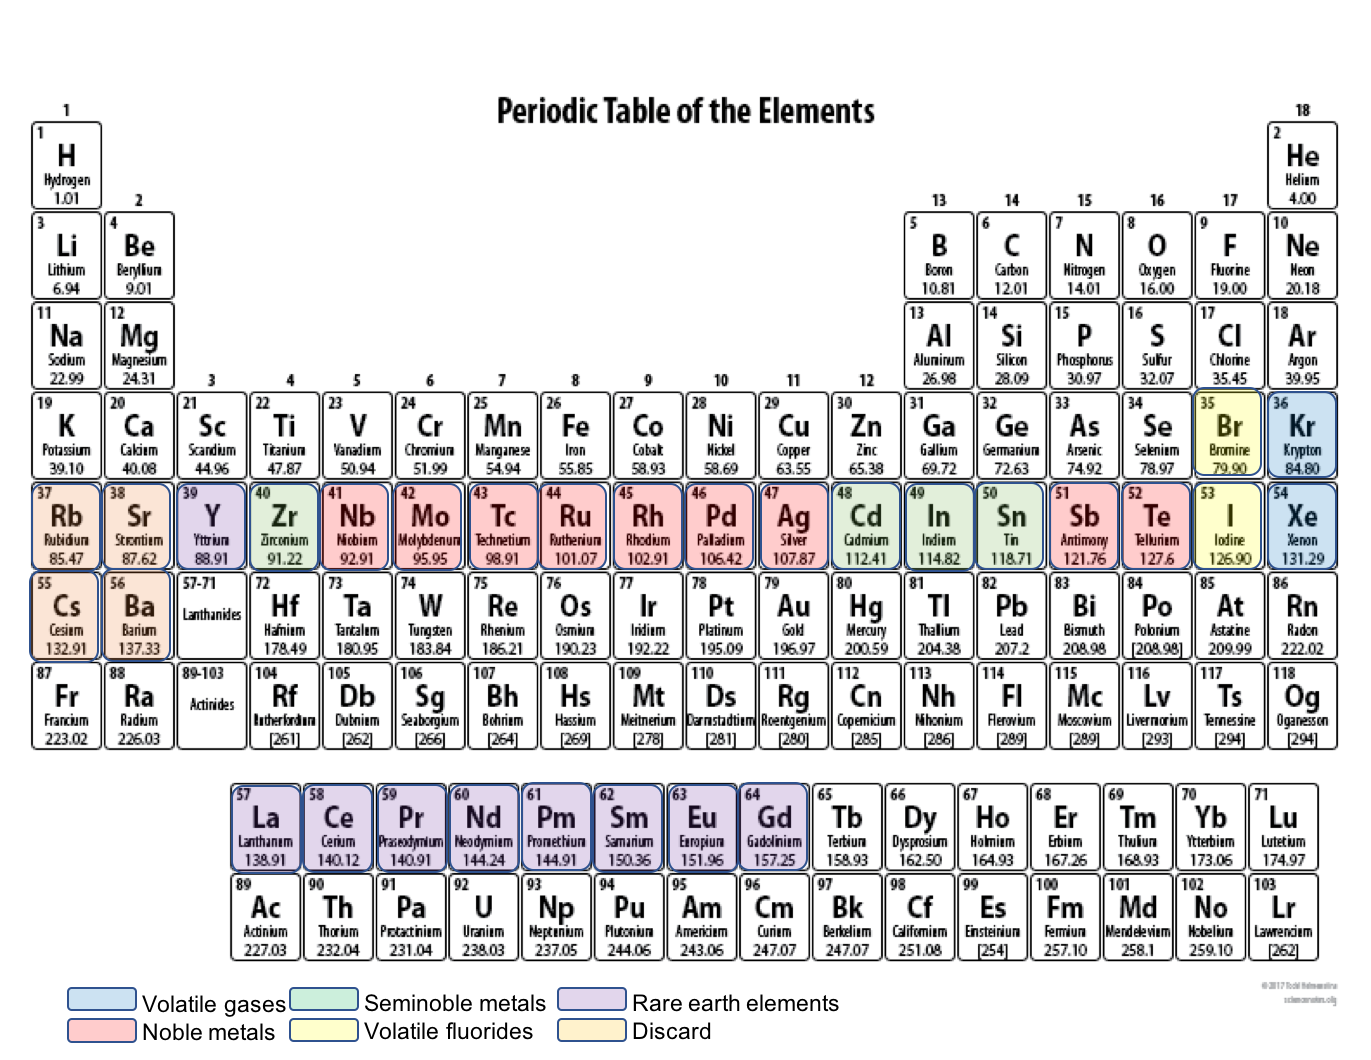
\includegraphics[width=6in]{periodic_table.png}\\
  \caption{Periodic table with highlighted fission products.}
  \label{fig:periodic_table_fp}
\end{figure} 

\FloatBarrier
\newpage

\subsubsection{Noble Gases}
Fission product noble gases Xe and Kr form no compounds in a MSR and are sparingly soluble in the carrier salt. Because of this, these noble gases tend to collect in any circulating voids contained in the flow loop. Many present and past MSR designs utilize this fact and include gas stripping processes which entrained bubbles in the carrier salt. Process equipment may also be permeable to fission product gases. In the case of the MSRE, moderator graphite was permeable and influences steady-state and transient noble gas behavior \cite{grimes1970}. Xenon is of particular interest due to its isotope ${}^{135}$Xe which has a neutron absorption cross section many orders of magnitude higher than the fissile material dissolved in the fuel. Xenon robs the reactor of neutrons and will eventually shut down the reactor if not properly handled. 

\section{VERA}
The Consortium for Advanced Simulation of Light Water Reactors (CASL) is the US Department of Energy's (DOE) first Energy Innovation Hub, a large collaboration among nuclear engineering research institutions and commercial partners around the globe, headquartered at ORNL. CASL's mission is to confidently predict the performance of existing and the next generation of advanced nuclear reactors \cite{casl}. In doing so, they have developed the Virtual Environment of Reactor Applications Core Simulator (VERA-CS), a collection of software tools utilized for modeling LWRs. VERA performs coupled multi-physics simulations involving reactor nuclear physics, thermal-hydraulics, LWR chemistry, isotopic depletion and fuel performance. In order to handle the industry's growing interest in advanced nuclear reactors, VERA-MSR is currently under development to extends its capabilities to model MSRs. In addition to the physics packages already supported in VERA, two more needed to be added, these include species transport and thermochemical state, as shown in Figure \ref{fig:multiphysicsMSR}.

 
For thermal-hydraulic calculations VERA uses CTF, a modernized version of COBRA-TF which was originally developed in the early 1980s by Pacific Northwest Laboratory \cite{zack2018}. CTF uses a two-fluid model broken up into three separate fluid fields: liquid film, liquid droplets and vapor, each with its own set of conservation equations. The governing sets of 9 equations is turned into 8 by assuming that liquid and droplet fields are in thermal equilibrium and share an energy equation. Discretization is done on a 3-D finite volume Cartesian mesh with scalar and momentum cells staggered on top of one another. The governing set of equations are formatted either using the full 3-D solution or using a sub-channel approach and are solved using the SIMPLE method \cite{salko2017}. After a CTF solves its governing set of mass, momentum and energy equations, temperature, pressure and the velocity fields are known, these values are then utilized in species transport. Temperature and pressure fields are required for two-phase interfacial area calculations. The fluid velocity field is used in the convection flux contribution for species transport.  

\vspace{12.7mm} %5mm vertical space

\begin{figure}[h]
  \centering
  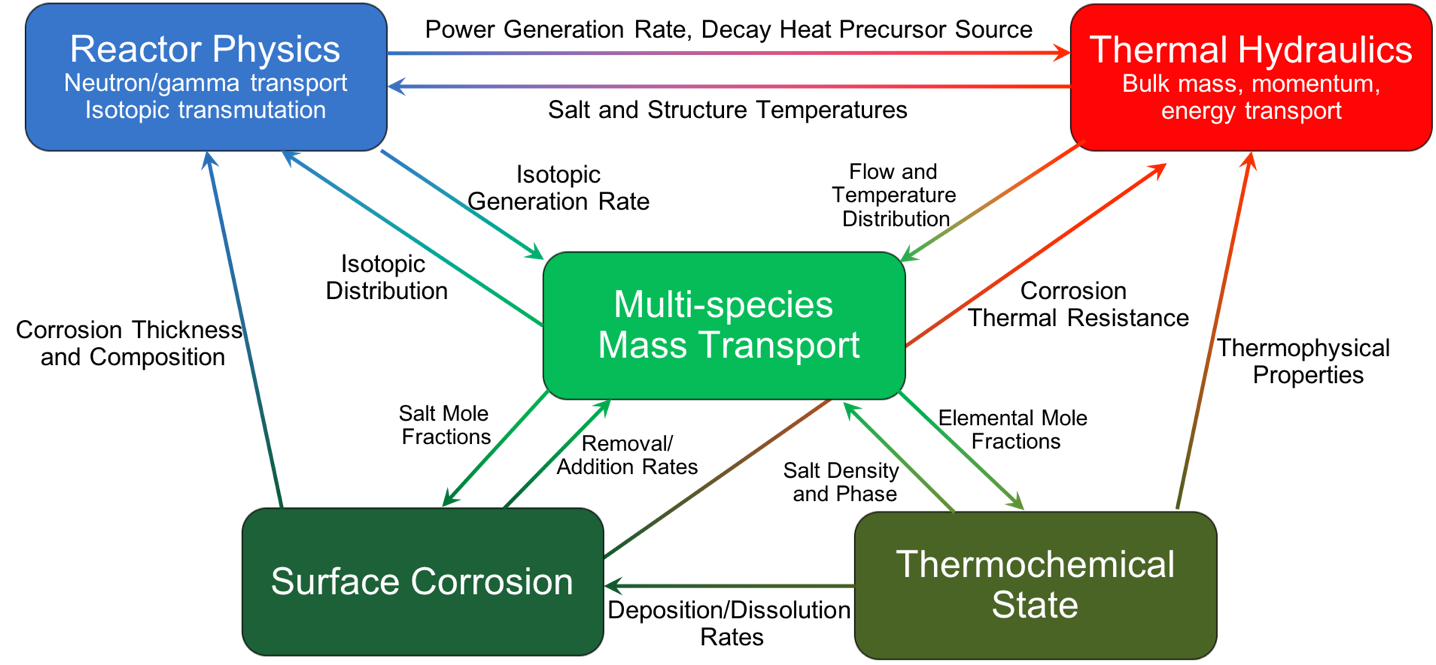
\includegraphics[width=6in]{images/multiphysics.png}\\
  \caption{Multi-physics simulations need for MSRs}
  \label{fig:multiphysicsMSR}
\end{figure}
    \chapter{Behavior of Volatile Fission Products }\label{ch:VFP_behavior}

Throughout the history of the MSRE many attempts were made to understand the behavior of fission products. This includes their overall chemical and transport methods in a molten salt environment. In this section we discuss lessons learned from the MSRE as well as some previous attempts at modeling xenon transport and fission product thermodynamic behavior. Much of the focus during the MSRE was to understand ${}^{135}$Xe transport. Xenon poisoning was a common metric used during the MSRE to compare the effects of system parameters, such as circulating void, mass transfer coefficient and bubble stripping efficiency. Poisoning is a function of xenon concentration and increases with increasing concentrations of xenon. When discussing changes in xenon poisoning, these changes are directly proportional to changes in xenon concentration in the reactor.  

This section focuses on the general species transport in a liquid and mass transfer from said liquid to circulating bubbles. When discussing the previous modeling attempts only phase coupling between liquid and gas phases will be shown. 
\section{Noble Gases}

Volatile gases are elements or compounds which presumably exist in the gaseous state and include fission products Xe, Kr and other gaseous fission products. In a fluoride system both Br and I can form volatile fluorides. Noble gases Xe and Kr are only sparsely soluble in the molten salt, because of this low solubility, Xe and Kr tend to leave the salt and enter any circulating gas bubbles. During  the MSRE, circulating gas bubbles existed under normal operating conditions with values ranging from 0.02 to 0.04 vol. \%. Significant changes in void fraction could be influenced by temperature, overpressure, and fuel-pump level \cite{engel1971}.
Noble gases also diffuse into process material. During MSRE operations, a graphite moderator was utilized in the reactor core. This graphite had a porosity which allowed noble gases and liquid salt to migrate inside, this migration is non-negligible when compared to other material migration mechanisms. As short-lived noble gases diffuse into the graphite, they decay or undergo transmutation. Once this process occurs, all daughter products remain in the graphite \cite{kedl1967}.  

\subsection{Effect of Circulating Voids}
Transport of volatile gases to circulating bubbles is an attractive mechanism for noble gas removal in MSRs. These circulating voids can then undergo gas removal operations followed by an off-gas processing system. Usually, off-gas removal systems utilize a charcoal decay method which generates a holdup time allowing for gases to decay into stable isotopes. As the noble gas concentration increases in the circulating voids, it is to be expected that removal of said gases should increase. This effective removal process is assumed to be largely controlled by the surface area of the circulating bubbles \cite{peebles1968}. 

Salt density was also affected by circulating voids. As void fractions in the reactor increase this decreased the amount of fissile material. This would then cause a decrease in fission reactivity. During MSRE operations a 1\% change in density would cause a 0.18\% or 0.45\% change in reactivity for ${}^{235}U$ and ${}^{233}U$ operations, respectively. Redox condition of the salt can also have an effect on void behavior through changes in surface tension and viscosity \cite{houtzeel1970}. 

\subsection{Cover Gas Solubility}

During MSRE operations two cover gases were used as a transfer medium for fission product gas removal, helium and argon. A model was developed to describe ${}^{135}Xe$ behavior, however when argon was substituted for helium as the cover gas, variation of steady-state xenon poisoning was observed \cite{engel1971}. This was due to the relative differences in cover gas solubility; argon is less soluble in the MSRE carrier salt than helium. 

Bubble life can widely vary depending on liquid pressure and cover gas solubility. When system pressure increases void fractions decrease due to compressibility and gas solubility. In these high-pressure regions, gas can transfer from the bubbles into the solution and back into the bubbles in low-pressure zones. Figures \ref{fig:time_dependent_void} and \ref{fig:equ_void} show the relative differences between argon and helium for the MSRE salt.

Figure \ref{fig:time_dependent_void} shows the void fraction as a function of time while varying pressure. In this case the initial pressure and void fraction are 20 psia and 1.5 vol\% respectively. At time zero the liquid is instantly pressurized to 70 psia then linearly decreases to 20 psia after 25 seconds. Figure \ref{fig:equ_void} shows the equilibrium void fraction vs liquid pressure. This figure shows the impact gas solubility can have on void fraction. Higher gas solubility means that under increased pressure the entire bubble can collapse thus allowing any species dissolved in the cover gas to redistribute into the carrier salt. Larger helium bubble also tended to retain their identity around the MSRE salt loop \cite{steffy1969}.

\vspace{12.7mm} %5mm vertical space

% differences in solubility for argon and helium
\begin{figure}[ht]
  \centering
  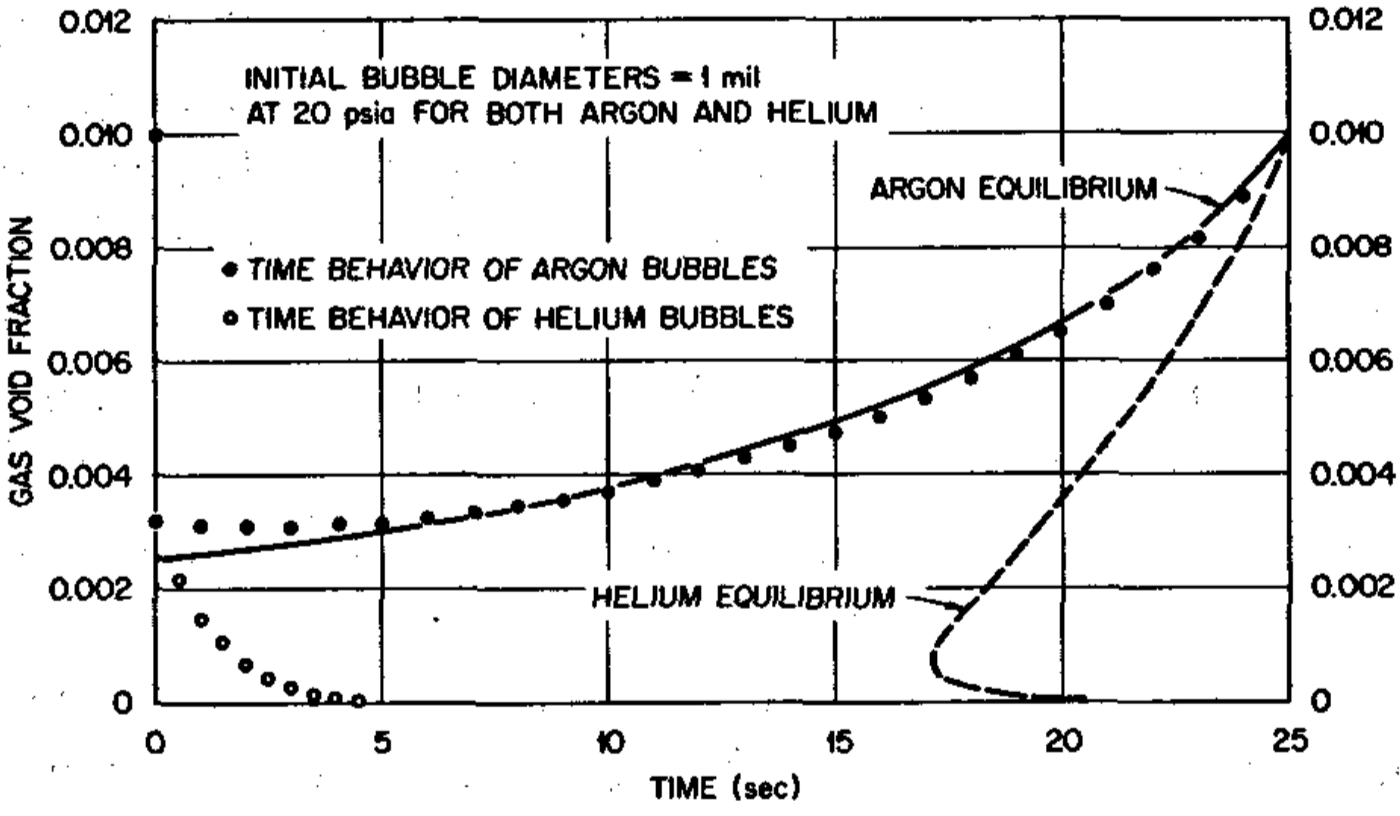
\includegraphics[width=4in]{time_dependent_void.png}\\
  \caption{Time dependent liquid pressure effects on gas void fraction. \cite{steffy1969}}
  \label{fig:time_dependent_void}
\end{figure} 


\newpage

\begin{figure}[ht]
  \centering
  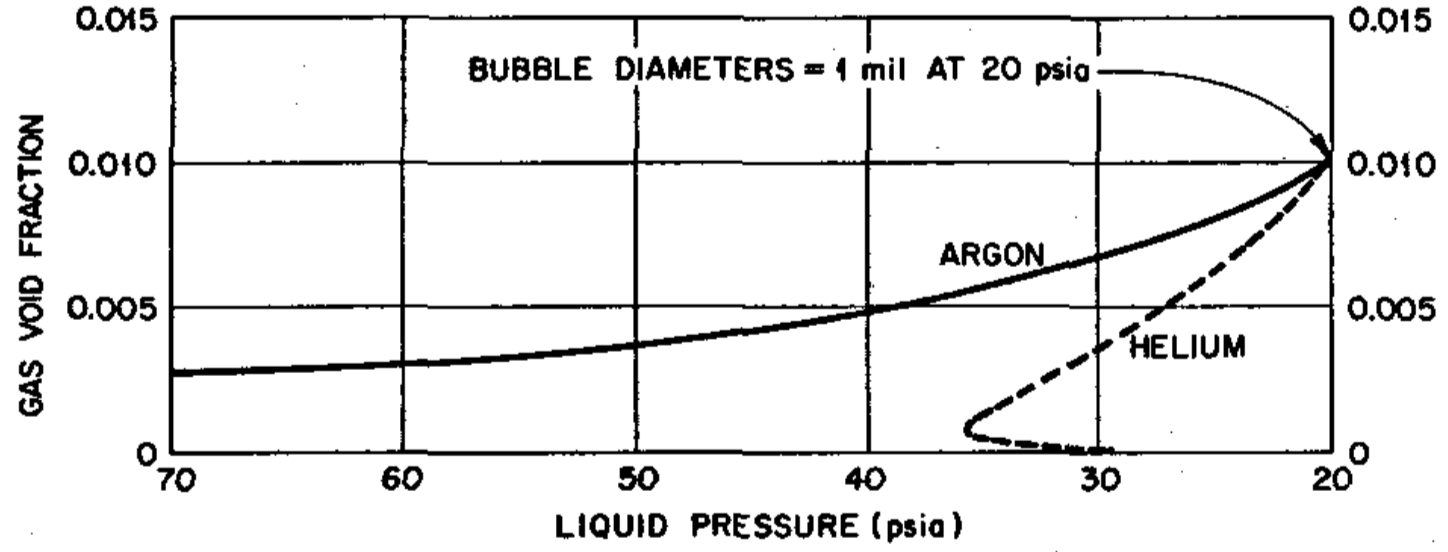
\includegraphics[width=4in]{equilibrium_void.png}\\
  \caption{Equilibrium void fraction vs. liquid pressure. \cite{steffy1969}}
  \label{fig:equ_void}
\end{figure} 



% Mass transport
\subsection{Noble Gas Transport}
As mentioned before, many attempts were made to understand the transport of ${}^{135}$Xe. This section lays out the mathematical models used during the MSRE to transport xenon. The same methods can also be used to model the migration of any volatile gases, assuming that the proper volumetric source terms are taken into account. 

% Mass transfer to moderatior
\subsubsection{Mass Transfer to Moderator}

Depending on reactor design, a moderator might be utilized in slowing down neutrons to induce thermal fissions. This moderator can be directly exposed to the circulating fuel salt, and therefore be subject to mass transfer to its surface along with subsequent diffusion into the material. It is important to note that all species included in the circulating salt are subject to mass transport on and into the moderator. This includes: fission products, fissile material and carrier salt. Three contributing factors that influence this rate include Reynolds number, moderator porosity and diffusion coefficients. As porosity and diffusion coefficient decrease, absorption rates into the moderator decrease. Typically, as Reynolds number increases mass transfer rates increase \cite{watson1962}. 

Pressure changes will not move salt into or out of moderator pores with any appreciable amount, so long as the pores are relatively small. Gas however will, and the rate will vary depending on the nature of the pressure change and the extent of pressure increase over the time interval. The amount of gas in the moderator is a function of the partial pressure in the carrier salt \cite{kedl1972}.

% Mass transfer to circulating voids
\subsubsection{Mass Transfer to Circulating Voids}
During the MSRE sigificant efforts were made to understand ${}^{135}$Xe poisoning. This treatment can be extended to any FP gas. The rate of FP gas migration (atoms per hour) into the circulating bubbles is represented by Equation \ref{eq:migration_rate_xe_MSRE_surface} \cite{houtzeel1967}.

\begin{equation}
    \text{Migration rate to bubbles} = h_{B}A_{B}(C_{S}^{X} - HRTC_{B}^{X})
    \label{eq:migration_rate_xe_MSRE_surface}
\end{equation}

In Equation \ref{eq:migration_rate_xe_MSRE_surface} $C_{s}^{X}$ and $C_{B}^{X}$ are the atomic concentrations of gas X in the salt and bubbles respectively. $A_{B}$ and $h_{B}$ are the interfacial area and mass transfer coefficient. H, R, and T are the Henry's law coefficient, universal gas constant and bubble temperature. Using a model developed in \cite{houtzeel1967} they estimated that small amounts of helium voids would have significant impact on the over all xenon distribution. This is evident from sample calculations indecating that with 0.01 circulating void fraction 98\% of the xenon would be in the bubbles and at 0.001 void, 83\% would be in the bubbles \cite{houtzeel1967}. Using a lumped mass model described in \cite{houtzeel1967}, calculations were preformed to estimate the change in xenon poisoning with mass transfer coefficient, mean bubble diameter and bubble stripping efficiency shown in Figures \ref{fig:MSRE_mass_tranfer}, \ref{fig:MSRE_bubble_size}, \ref{fig:MSRE_bub_strip}.

\vspace{12.7mm} %5mm vertical space

\begin{figure}[ht]
  \centering
  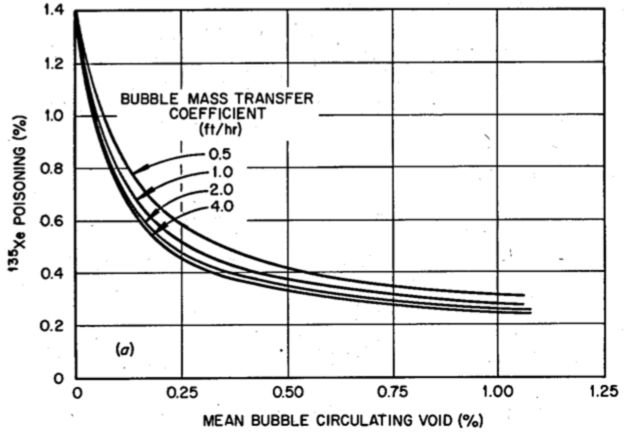
\includegraphics[width=4in]{images/MSRE_mass_transfer_coeff.png}\\
  \caption{Affect of mass transfer coefficient on xenon poisoning}
  \label{fig:MSRE_mass_tranfer}
\end{figure} 

\newpage

\begin{figure}[p]
  \centering
  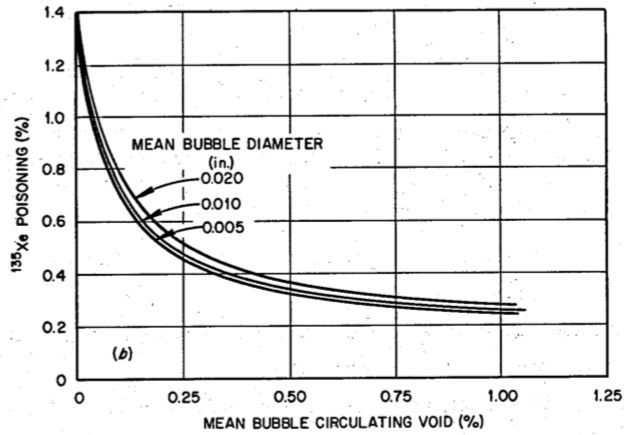
\includegraphics[width=4in]{images/MSRE_mean_bub_dia.png}\\
  \caption{Affect of mean bubbles diameter on xenon poisoning}
  \label{fig:MSRE_bubble_size}
\end{figure} 

\begin{figure}[p]
  \centering
  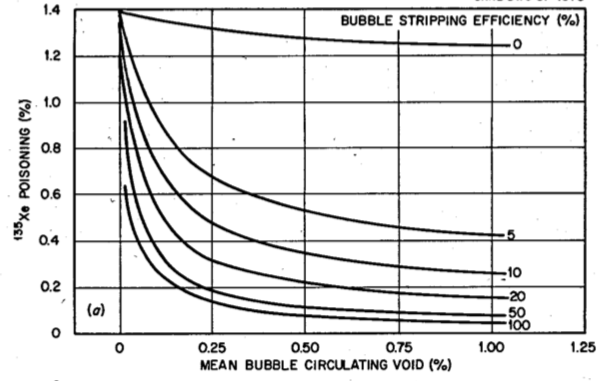
\includegraphics[width=4in]{images/MSRE_bub_stripping.png}\\
  \caption{Affect of bubble stripping efficiency on xenon poisoning}
  \label{fig:MSRE_bub_strip}
\end{figure} 

\FloatBarrier
\newpage

From Figures \ref{fig:MSRE_mass_tranfer} and \ref{fig:MSRE_bubble_size} it was concluded that xenon poisoning is a rather weak function of mass transfer coefficient and bubble diameter. Bubble stripping efficiency has the highest impact on xenon poisoning. These calculations were preformed under the assumption of constant bubble diameter and void fraction. 


% Noble metals
\section{Noble Metals}

The noble metals represent a class of fission products that are reduced by the fuel salt resulting in their existence to be in the solid metallic state.  These reduction reactions are fast and as soon as the noble metals are born they quickly undergo reaction to become neutral metallic nanoparticles \cite{kedl1972}. Reactions of noble metals occur with the fissionable isotope in the fuel salt or components of vessel vie the sample reaction shown in Equation \ref{eq:fp_reduction}. For a structural metal, shown in \ref{eq:metal_reduction}.  

 \begin{equation}
	M^{+n} + nUF_{4} \rightleftharpoons nUF_{3} + MF_{n}
	\label{eq:fp_reduction}
\end{equation}

 \begin{equation}
	M^{+n} + E \rightleftharpoons E^{+n} + M
	\label{eq:metal_reduction}
\end{equation}

In Equation \ref{eq:fp_reduction} fission product $M$ is being reduced by $UF_{4}$ and in Equation \ref{eq:metal_reduction}, $M$ is being reduced by a structural metal $E$. Structural metal $E$ will most likely form an ionic compound with free anions from the carrier salt. 

During MSRE operations, these particles were also found to deposit in the off-gas system and pump bowl. It has also been seen that these noble metals tend to accumulate on vessel and heat exchanger surfaces \cite{kedl1972}. This previously described behavior is due to the fact noble metals have properties much similar to surface active agents which tend to gather around liquid-gas interfaces \cite{kedl1972}. 

% Thermodynamic background
\subsection{Thermodynamic Background}

Oxidation and reduction reactions occur within the molten salt with fission products, fissile material and the metal container. These reactions go on to produce corrosion products and noble metals. A number of fission products may exist as noble metals or as salt seekers and their fate depends upon the redox condition of the salt. 

Redox reactions involve the transfer of electron between reacting species. The species that receives electrons is reduced and the species that donates the electrons is oxidized. The redox condition is often used in referring to a systems propensity to reduce or oxidize a given species. During MSRE operations this term was used when referring to a fission product's tendency to reduce to their metallic state or for the corrosion of container metals \cite{olander2002}. Controlling these reactions (conditioning the salt) is accomplished by controlling the salts tendency to reduce. For either fluoride or chloride based salts, this is done by controlling the potential of diatomic gases anions. 

As mentioned in section \ref{source_terms}, because the reactor operates at such a high temperature, a pseudo equilibrium assumption can be made about the salt. This means that thermodynamic equilibrium is set and reaction equilibrium concentrations can be calculated. Some noble metal reactions almost reach completion while others do not. The ones that do not are known as semi noble metals and their reactivity will be dependent on the redox condition of the salt. In many previous MSR reports, redox condition was a loose term used to describe an elements propensity to undergo redox reactions. Redox condition of the salt is correlated to the chemical potential of the anion either Cl- or F- of the carrier salt \cite{olander2002}.  

For a given reversible chemical reaction,

% General chemical reaction
 \begin{equation}
	v_{A}A + v_{B}B \rightleftharpoons v_{C}C + v_{D}D
	\label{eq:gen_chem_rxn}
\end{equation}

the law of mass action says that,

% Law of mass action
 \begin{equation}
	K_{a} = \prod a_{i}^{v_{i}} = \frac{a_{C}^{v_{C}}a_{D}^{v_{D}}}{a_{A}^{v_{A}}a_{B}^{v_{B}}}
	\label{eq:mass_action}
\end{equation}

therefor at equilibrium and standard state the term on the right-hand side will equal a constant ($K_{a}$) where  is activity and  is stoichiometric coefficient. Chemical activity for the liquid phase can be defined in terms of a substances activity coefficient ($\gamma$) and molar fraction ($x$). 

% activity coefficient
 \begin{equation}
	a_{i} = \gamma_{i}x_{i}
	\label{eq:activity}
\end{equation}

For an ideal solution, the activity coefficient is equal to one and for the gas phase, mole fraction can be replaced with partial pressure. The reaction quotient is related to the Gibbs energy of reaction by, 

 \begin{equation}
	K_{a} = \exp \bigg( \frac{-\Delta G_{rxn}^{o}}{RT} \bigg)
\end{equation}

The change in Gibbs energy with reaction is defined as,

% gibbs reaction
 \begin{equation}
	\Delta G_{rxn}^{o}(T,P) = \Delta G_{f}(products) - \Delta G_{f}(reactants)
	\label{eq:gibbs_rxn}
\end{equation}

The summation of the Gibbs energy of formation for products minus reactants. Gibbs energy is a thermodynamic property which is defined as, 

% gibbs energy
 \begin{equation}
	G = H - TS
	\label{eq:gibbs}
\end{equation}

where $H$ is enthalpy, $T$ is temperature and $S$ is entropy. The change in Gibbs energy is equal to the maximum non-expansion work accompanying a process at constant temperature and pressure. When solutions undergo reactions, the extent is driven toward equilibrium by minimizing the Gibbs energy. This means that for a multicomponent mixture undergoing reactions, the equilibrium species concentrations can be calculated by minimizing the total Gibbs energy of the system. 

In a classical thermodynamic chemical potential is defined as the change in Gibbs energy with number of moles.

% chemical potential
 \begin{equation}
	\Delta \bar{G_{i}^{o}}  = \mu_{i} =  \frac{\partial (nG)}{\partial n_{i}}
	\label{eq:chemical_potential}
\end{equation}

When examining a chemical reaction, the potential of a particular species can be solved for by combining the relations for equilibrium constant and the definition of activity. For example, take reaction shown in equation \ref{eq:gen_chem_rxn}. The law of mass action shows.

 \begin{equation}
	\exp \bigg( \frac{-\Delta G_{rxn}^{o}}{RT} \bigg) = \frac{a_{C}^{v_{C}}a_{D}^{v_{D}}}{a_{A}^{v_{A}}a_{B}^{v_{B}}}
\end{equation}

The chemical potential for reactant A is,

% chemical potential for A
 \begin{equation}
	\Delta \bar{G_{i}^{o}}  = RT\ln(a_{A}) = \frac{1}{v_{A}} \bigg[ RT\ln \bigg( \frac{a_{C}^{v_{C}}a_{D}^{v_{D}}}{a_{B}^{v_{B}}} \bigg) + \Delta G_{rxn} \bigg]
	\label{eq:chemical_potential_A}
\end{equation}

% Noble metal transport
\subsection{Noble Metal Transport}

One of the key requirements for understanding noble metal transport is to first understand their behavior relative to the fluid velocity field. The homogeneous equilibrium model is a simple mixture model which describes the multiphase model as a pseudo single-phase mixture in thermodynamic equilibrium. This model includes assumptions much like the ones which were used to describe two-phase liquid-bubble transport. The primary being that the relative velocities between each phase are zero and each phase is in thermodynamic equilibrium with another. 

Many different surface environments exist in a molten salt loop, which include; moderator, heat exchanger, reactor wall, piping/process equipment and liquid-gas interfaces. Many of these surfaces may not be in thermodynamic equilibrium with the bulk fluid, creating temperature gradients which can affect the amount of noble metal which can deposit. One example of this is in the heat exchanger where bulk fluid temperature is changing as a function of heat exchanger length and fluid velocity. Solubility, which is a function of temperature, begins to change which can lead to a supersaturated state of the liquid solution, leading to increased noble metal deposition. Other processes which can affect surface deposition rates include fluid turbulence, torturous paths and surface area for transfer. 

For noble metal deposition on surfaces, the same convention in which the boundary layer is ignored and a linear convection boundary condition is utilized, equaiton \ref{eq:convection_boundary_condition}. The trick for using this assumption is knowing the mass transfer coefficient  and the surface concentration. Surface concentration can only be assessed if certain assumptions are used. These assumptions deal with the noble metals propensity to stick and stay on the surface and diffuse into the material. A common assumption is to treat the surface material as an infinite sink, making the concentration at the surface zero. This assumption can be used when solving a steady state problem where the surface concentration is unknown. In a time dependent problem, the surface concentration can be assumed to be equal to zero or a given constant. Then for all times greater the surface concentration would be the integral of the flux from zero to the current time or the previous time step. 

An interesting note that comes into play when discussing mass transfer in a saturated system is the affect heterogeneous nucleation has on transfer coefficient. Depending on how the mass transfer coefficient is obtained, nucleation may not be included in the transfer rate. This most then be added to the migration model to obtain a more accurate model. However, if the liquid solution never reaches a point of super saturation, then nucleation does not occur. 

% Noble metal behavior
%\subsection{Noble metal behavior}

%Observations made during the MSRE impart great insight into the general behavior of noble metals in a molten salt environment. During operations, noble metals played a role in many key processes which effected system wide behavior. The behavior includes; deposition on liquid-gas interfaces, plating to container surfaces, and entrapment in the off-gas system. 

%\subsubsection{Liquid-gas interactions}

%As previously noted, noble metals have a tendency to migrate to liquid gas interfaces. This tendency to collect on liquid-gas interfaces follows the same physical model as was surface deposition, however the question remains in finding the surface concentration. During MSRE operation an analytical model was developed for determining migration of noble metals \cite{kedl1972}. From these models, as well as experimental results, it was found that noble metals did not have a tendency to stay on the bubble surface once they became attached. 




    \chapter{Governing Equations} \label{ch:gov_eqns}

The governing species transport equations are implemented into a coding structure based on a finite volume discretization. First the integral volume formulation of the species transport equation is derived. Next volumetric source terms for isotopic species, boundary conditions and phase coupling are discussed. Finally, the interfacial area tracking method is derived.

\section{Conservation of species for multi-phase flow}
Consider the fixed control volume for two phase flow show in Figure \ref{fig:gen_control_volume}.

In deriving the conservation of species relation we will first start with the relation for a system with a single phase. Let \textit{C} be the conserved quantity of interest in amount per unit volume and let \textit{F} be the flux, amount per unit area per time passing through the unit normal surface of \textit{V}. If the quantity \textit{C} is being generated in control volume \textit{V} then let its generation rate be denoted by ${C_{V}}$. Equation \ref{eq:gen_species_con_integral_volume} represents the conservation of species in a fixed control volume. 


% Control Volume
\begin{figure}[ht]
  \centering
  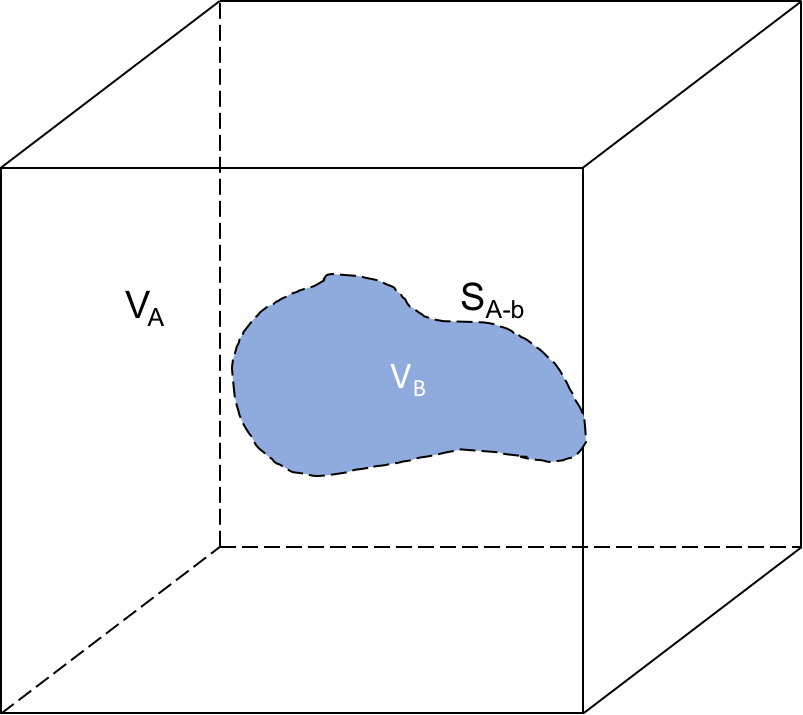
\includegraphics[width=3in]{two_phase_cell_volume.png}\\
  \caption{General control volume.}
  \label{fig:gen_control_volume}
\end{figure} 

% General equation species integral volume
\begin{equation}
	\frac{\partial }{\partial t}\iiint_V C \,dV = -\iint_S n \cdot F \,dS + \iiint_V C_{V} \,dV
	\label{eq:gen_species_con_integral_volume}
\end{equation}

The differential operator in the first term of Equation \ref{eq:gen_species_con_integral_volume} can be brought inside the integral by applying Leibniz integral rule shown below.

% Application of Leibniz rule
\begin{equation}
	\frac{\partial }{\partial t}\iiint_V C \,dV = \iiint_V \frac{\partial C}{\partial t}\,dV
\end{equation}

This simplifies equation \ref{eq:gen_species_con_integral_volume} to 

% Plugging in Leibniz rule to the general equation
\begin{equation}
	 \iiint_V \frac{\partial C}{\partial t}\,dV = -\iint_S n \cdot F \,dS + \iiint_V C_{V} \,dV
	\label{eq:gen_species_con_integral_volume_leibniz}
\end{equation}

Let a phase be a region where \textit{C} is a continuous function and interfaces are surfaces which can introduce discontinuities in \textit{C}. Using Equation \ref{eq:gen_species_con_integral_volume_leibniz}, Leibniz integral rule is applied to the time derivative of each phase volume separately. 

% apply Leibniz rule to volume A
\begin{equation}
	\frac{\partial }{\partial t}\iiint_{V_{A}} C \,dV = \iiint_{V_{A}} \frac{\partial C}{\partial t}\,dV + \iint_{S_{I}} C_{A} n_{I} \cdot v_{I} \,dS
	\label{eq:leibniz_rule_volA}
\end{equation}

% apply Leibniz rule to volume B
\begin{equation}
	\frac{\partial }{\partial t}\iiint_{V_{B}} C \,dV = \iiint_{V_{B}} \frac{\partial C}{\partial t}\,dV - \iint_{S_{I}} C_{B} n_{I} \cdot v_{I} \,dS
	\label{eq:leibniz_rule_volB}
\end{equation}

The last term in Equations \ref{eq:leibniz_rule_volA} and \ref{eq:leibniz_rule_volB} take into account the velocity of the phase interface. In equation, this contribution is subtracted due to the unit normal point in the opposite direction. These two equations can be added together to represent the entire volume. 

% Leibniz rule for vol A, B
\begin{equation}
	 \iiint_V \frac{\partial C}{\partial t}\,dV = -\iint_S n \cdot F \,dS + \iiint_V C_{V} \,dV + \iint_{S_{I}} (C_{A} - C_{B}) n_{I} \cdot v_{I} \,dS
	\label{eq:two_phase_time_term}
\end{equation}

The last term in Equation \ref{eq:two_phase_time_term} is only present when  the interface is moving and \textit{C} is discontinuous. If a source term is present in the interface then the rate of formation per unit area of interface is ${C_{S}}$. 

% combining all terms for a two phase system
\begin{equation}
	 \iiint_V \frac{\partial C}{\partial t}\,dV = -\iint_S n \cdot F \,dS + \iiint_V C_{V} \,dV + \iint_{S_{I}} (C_{A} - C_{B}) n_{I} \cdot v_{I} \,dS + \iint_{S_{I}} C_{S}   \,dS
	\label{eq:two_phase_Intarea_source}
\end{equation}

When more than two phases are present, then the last two terms in Equation \ref{eq:two_phase_Intarea_source} are represented as summations for all phases present. The integral formulation at an interface can also be represented by Equation \ref{eq:alt_integral_surface} \cite{deen2016}.

% representing the source term at an interface
\begin{equation}
	 \iint_S [(F - CV_{I})_{B} - (F - CV_{I})_{A})]\,dS = \iint_S C_{S} \,dS
	\label{eq:alt_integral_surface}
\end{equation}

Where the term $F - CV_{I}$ is the flux relative to the interface. For an arbitrary number of phases, species can be represented as a balance over each phase volume. 

% two-phase volume equation
\begin{equation}
	\iiint_{V} \frac{\partial \alpha_{k}C_{k} }{\partial t}\,dV = -\iint_S n \cdot F_{k} \,dS + \iiint_V \alpha_{k}C_{V,k} \,dV + \iint_{S_{j}} C_{S_{k}} \,dS
	\label{eq:two_phase_species_con_integral_volume}
\end{equation}

These set of equations are the fundamental relations regarding the conservation of species for a multi-phase system. In the case of a multi-component system, these same relations apply, however care must be taken when developing inner species interactions and phase migration. 

% Source terms
\section{Understanding Volumetric Source Terms} \label{source_terms}
To understand the behavior for fission products it is first necessary to understand the source and sink terms for each product of interest. For a general reactor design these terms are represented in Table \ref{tab:volume_source_terms}\cite{houtzeel1967}. 

% table of source and sink terms
\begin{table}[htbp!]
   \caption{\label{tab:volume_source_terms} Source and sink terms for chemical species and elemental isotopes}
   \centering
   \begin{tabular}{l llll}
   \hline
   \textbf{Source/Sink} & \textbf{Mechanisms involved}\\
   \hline 
   Direct from fission & Neutron flux, fission yield \\[1ex]
   Decay from parent atom & Decay constant \\[1ex]
   Transmutation & Neutron flux, microscopic cross-section \\[1ex]
   Phase/material migration & mass transfer, diffusion theory \\[1ex]
   Removal/addition system & Removal efficiency, addition rate \\[1ex]
   Chemical reaction & Reaction rate, thermodynamic equilibrium \\[1ex]
   \hline
   \end{tabular}
\end{table}

To understand the fate of volatile fission products in a MSR we must first derive a rate balance for each species of interest. Molten salts are characterized by having a melting point with reactors operating at temperatures well above liquid temperatures. Because of this, it is assumed that all chemical reaction occurring in the salt happens instantaneously \cite{baes1974}\cite{kedl1972}. This also leads to the next assumption, that the salt is in a pseudo equilibrium state at almost all times. This allows for the calculation of thermophysical properties with the use of Gibbs free energy minimization. 

% Nuclear interactions
\subsection{Nuclear Interactions}
Because volumetric generation rates depend on nuclear reactions, it is important to first understand the mechanisms governing the physical interaction of particles and isotopes. 

% Importance of decay chains
\subsection{Importance of Decay Chains}
Most fission products are atomically unstable and will decay into other elements based on half-lives and decay chains, so these other elements may be created from these decays or separately as direct fission products. This greatly complicates fission product accumulation and accounting, and influences the ultimate disposition. Consider the following decay scheme \cite{kedl1972}:

\begin{equation}
	Fission \space (\gamma_{_{Kr}})\rightarrow Kr \rightarrow Rb \rightarrow Sr \rightarrow Y \rightarrow Zr \rightarrow Nb \rightarrow Mo \rightarrow
\end{equation}

In this scheme Kr is a noble gas, Rb, Sr, Y, Zr are salt seekers, Mo is a noble metal with Nb being either a noble metal or salt seeker depending on redox condition of the carrier salt.  This demonstrates the need to understand fission product decay chains. Likewise, especially for an MSR, an understanding of half-lives relative to the mass transport process cycle times is also needed. For example, if one of the precursors is removed from the system then so will all other elements. However, if removal time is short compared to the half-life then the chain is more likely to proceeded and produce the elements further down the decay chain. 

% Direct from fission
\subsection{Direct Yield from Fission}
Generation rate from fission is a function of neutron flux and fission yield shown in Equation \ref{eq:vol_fission_term} \cite{houtzeel1967}.

\begin{equation}
	rate = \gamma_{i}\Sigma_{f}\phi
	\label{eq:vol_fission_term}
\end{equation}

Where $\gamma_{i}$, $\Sigma_{f}$ and $\phi$ are fission yield, macroscopic fission cross section and neutron flux. The major contribution from this term will be in the liquid salt phase. So, to understand where this term exists one must follow the dissolved salt. If the salt has a tendency to migrate into any process equipment, such as a moderator, for example, then the moderator material will have a fission source term. Fission yields and macroscopic cross sections are not constant, whereby the fission yield is dependent on the nuclear fuel used, and the macroscopic cross section is a function of temperature, material composition and density, and neutron energy. 

% Generation from decay
\subsection{Generation from Decay}
Generation and loss rates due to decay are a function of decay constant and isotope number density, shown in Equation \ref{eq:vol_decay_term} \cite{houtzeel1967}.

\begin{equation}
	rate = + \sum_{j=1}^{N} \lambda_{j\rightarrow i}N_{j} - \sum_{j=1}^{N} \lambda_{i\rightarrow j}N_{i}
	\label{eq:vol_decay_term}
\end{equation}

Where $\lambda$ and $N$ are the decay constant and atomic number densities, respectively. The decay constant is a natural constant and only dependent on the isotope of interest. As noted above, nuclear decay can be both a source and sink term.  If the isotope of interest $i$ is not stable then it will decay into another isotope $j$, making it a sink. Alternatively, if isotope $i$ is being generated from the decay of its parent $j$, then it becomes a source term. 

% Generation from transmutation
\subsection{Generation from Transmutation}
Generation from transmutation is a function of neutron flux, number density and microscopic cross section, as shown in Equation \ref{eq:vol_trans_term} \cite{houtzeel1967}.

\begin{equation}
	rate = + \sum_{j=1}^{N} \sigma_{j\rightarrow i}N_{j}\phi - \sum_{j=1}^{N} \sigma_{i\rightarrow j}N_{i}\phi
	\label{eq:vol_trans_term}
\end{equation}

Where $\sigma_{i\rightarrow j}$, $N_{i}$, and $\phi$ are microscopic cross section for the transmutation of isotope $i$ into $j$, or vice versa, atomic number density and neutron flux.  Similar to the generation from decay, a summation is needed to account for all isotopes that can transmute into isotope $i$ or transmute from isotope $i$ into another isotope $j$. Note that the macroscopic cross section is the product of a number density and a microscopic cross section, thus, microscopic or macroscopic cross sections are functions of temperature and neutron energy.

% Removal rate
\subsection{System Removal and Addition}
This term is dependent on the MSR design and must be evaluated for each design case. A simple example of removal rate from salt is shown in Equation \ref{eq:vol_removal_term}.

\begin{equation}
	rate = S_{eff}\dot{M}_{i}
	\label{eq:vol_removal_term}
\end{equation}

Where $S_{eff}$ and $\dot{M}_{i}$ are system removal efficiency and mass flow rate of species $i$. In general, the system removal coefficient can be defined in a number of ways ($i.e.,$ volumetric or mass flow rate) so the appropriate conversions must be taken.  

% Boundary conditions
\section{Boundary Conditions and Phase Coupling}
In this work, boundary conditions are defined as the mathematical formulation of physical phenomena that occur across phase/material boundaries in the solution domain. This can include phase migration ($i.e.,$ species dissolving or absorbing out of solution) and material migration, such as species plating out to a solid surface and or material migrating from liquid to solid surfaces.  For any boundary (liquid-gas, liquid-solid, solid-gas), Equation \ref{eq:alt_integral_surface} is valid. In the absence of bulk movement across the boundary the normal component of the velocity in either phase is equal to the normal component of the interfacial velocity \cite{deen2016}. This simplifies the flux term \textit{F} to only the diffusive flux component. 



\begin{equation}
	J_{in_{2}} - J_{in_{1}} = C_{S_{in}}
\end{equation}

Here, $J$ is the flux from either side of the surface and $C_{S_{in}}$ is a surface generation rate. If there are no surface source terms at the surface then the two diffusive fluxes are equal to one another. 

%\subsection{Diffusion fluxes}

For binary and mixtures, Fick's Law can be used when determining the species diffusive flux. Fick's Law describes the flux as a relation of a diffusion coefficient multiplied by the gradient of species concentration across a spatial length shown in Table \ref{tab:ficks_law} \cite{deen2016}.

For multi-component mixtures a pseudo-binary approximation can be used. In the assumption, a mixture of species is dissolved in a mixture where their concentrations dilute and it is assumed that they only interact with the solvent in which they are dissolved.

% two-phase interfaces
\subsection{Two-phase Interface}

In two-phase systems, the transfer of a species will continue along an interface until an equilibrium is reached. One common mechanism which describes this process is commonly known as two-film theory or two-resistance theory. Transport across an interface can be broken down into three steps.

\vspace{12.7mm} %5mm vertical space

 % table of ficks law for difference reference velocities. 
\begin{table}[htbp!]
   \caption{\label{tab:ficks_law} Fick's Law for various units}
   \centering
   \begin{tabular}{l ll}
   \hline
   \textbf{Reference velocity} & \textbf{Diffusive flux}\\
   \hline 
   ${\textbf{v}_{mass}}$ & $J =  -\rho D_{AB} \nabla \omega_{A}$ \\[1ex]
   ${\textbf{v}_{molar}}$ & $J =  -C D_{AB} \nabla x_{A}$ \\[1ex]
   \hline
   \end{tabular}
\end{table}

\newpage

\begin{enumerate}
	\item Transport of species from bulk of phase 1 to phase 1 interface
	\item Transport across the interface
	\item Transport from phase 2 interface to phase 2 bulk
\end{enumerate}

The two-resistance theory assumes that the rate for the overall transfer is determined from rate at which a species diffused from bulk to interface and from interface to bulk. In other words, the resistance transport across an interface in negligible \cite{wilson1969}. 

At phase interfaces, a local equilibrium does not imply equal concentrations on both sides of the interface, as shown in Figure \ref{fig:general_phase_interface}. The two concentration are however, related to one another by the partition coefficient \cite{deen2016}. The patrician coefficient $K_{P,i}$ is calculated based on the relative solubility of species i in the two phases. For a liquid-gas interface, Henry's law can be used and is shown in Equation \ref{eq:partition_coefficient}.

 \begin{equation}
	C_{i,1} = K_{P,i}C_{i,2}
	\label{eq:partition_coefficient}
\end{equation}

\begin{figure}[ht]
  \centering
  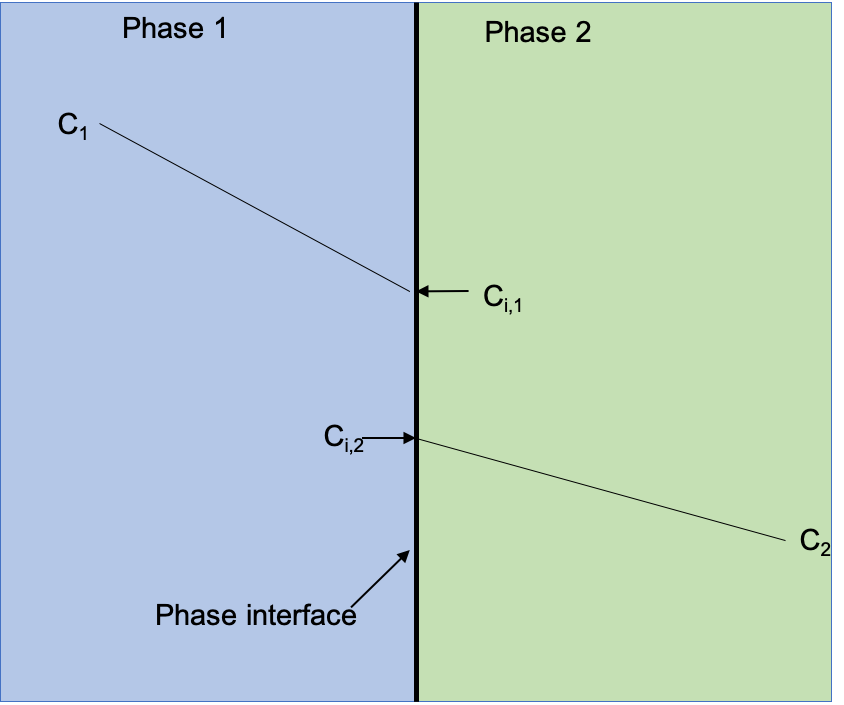
\includegraphics[width=3.2in]{images/general_phase_interface.png}\\
  \caption{Concentration profile across an interface}
  \label{fig:general_phase_interface}
\end{figure} 

\newpage

In situations where there is no phase change (i.e. no bulk flow across the interface) a convection boundary condition can be applied \cite{deen2016}. 

 \begin{equation}
	J_{in,2} =J_{in,1} = k_{2}(C_{in,2} - C_{bulk}) = k_{1}(C_{bulk} - C_{in,1})
	\label{eq:convection_boundary_condition}
\end{equation}

Equation \ref{eq:convection_boundary_condition} states that the flux across a boundary is proportional to the difference in concentration between the bulk fluid in phase k and the interface multiplied by the mass transfer coefficient $k_{ci}$. It is important to note that the driving force for species transport is the concentration only in the phase in question. Instead of using individual mass transfer coefficients, Equation \ref{eq:convection_boundary_condition} can also be represented using overall mass transfer coefficients $K_{i}$ \cite{bird2006}.

 \begin{equation}
	J_{in,2} =J_{in,1} = K_{2}(C_{e,2} - C_{bulk}) = K_{1}(C_{bulk} - C_{e,1})
	\label{eq:overall_convection_boundary_condition}
\end{equation}

$C_{e,2}$ and $C_{e,1}$ represent the equilibrium concentration in either phase. Using Equations \ref{eq:partition_coefficient}, \ref{eq:convection_boundary_condition} and  \ref{eq:overall_convection_boundary_condition} the following expression is obtained to relation single-phase and two-phase mass transfer coefficients for a liquid-gas system.

\begin{equation}
	\frac{1}{K_{G}} = \frac{1}{k_{G}} + \frac{m}{k_{L}}
	\label{eq:gas_phase_resistance}
\end{equation}

\begin{equation}
	\frac{1}{K_{L}} = \frac{1}{k_{L}} + \frac{1}{mk_{G}}
	\label{eq:liq_phase_resistance}
\end{equation}

Where \textit{m} is derived using Henry's law. For processes in which $ m >> 1$, $ \frac{1}{mk_{G}} $ approaches zero and mass transfer is liquid-phase controlled. On the other hand, if $ m << 1$, $ \frac{1}{mk_{G}}$ becomes very large, making the system gas-phase controlled. For systems which obey Henry's Law, the over all mass transfer coefficient can be represented by

 \begin{equation}
	\frac{1}{K_{L}} = \frac{1}{k_{L}} + \frac{HRT}{k_{G}}
\end{equation}

Therefore, if the Henry's law constant is very small i.e. the chemical species is sparsely  soluble in the liquid, then the contribution from $k_{G}$ is small and can be ignored. 

For a species i initially in the gas phase or gas bubbles, the rate at which i migrates into the liquid phase is modeled using Equation \ref{eq:gas_side_coupling}, where $a$ and $V$ are interfacial area and volume.

\begin{equation}
    \frac{\partial C_{i}^{g}}{\partial t} = \frac{Ka}{V}\Big[C_{i}^{l}  - C_{i}^{*}\Big]
    \label{eq:gas_side_coupling}
\end{equation}

The equilibrium concentration $C_{i}^{*}$ in the liquid is determined using Henry's law. In the case for a gas that is insoluble in the liquid, $H \rightarrow 0$ meaning that the only changed in concentration is due to migration from the liquid side. Because the fluxes are equal across both boundary's, the liquid side phase migration is governed by Equation \ref{eq:liq_side_coupling}.

\begin{equation}
    \frac{\partial C_{i}^{l}}{\partial t} = \frac{Ka}{V}\Big[C_{i}^{*} - C_{i}^{l}\Big]
    \label{eq:liq_side_coupling}
\end{equation}

In the case of a gas born inside of a liquid solution Equation \ref{eq:liq_side_coupling} governs its migration into the bulk gas phase. If the gas is insoluble in the liquid then again $H \rightarrow 0$ and its migration rate is governed by the concentration in the liquid and the mass transfer coefficient. 


% Mass transfer coefficients
\section{Mass Transfer Coefficients}
Mass transfer coefficients are of great importance to the understanding of interface mass transport. There are many different ways in which mass transfer coefficients can be derived. For simple situations, mass transfer coefficients can be derived using first principles \cite{perry2007}. However, in industrial applications most of these coefficients are empirically defined from experimental data. In many situations, a number of corrections may exist and one must be careful to use the appropriate coefficients. The Perry's Chemical Engineers' Handbook \cite{perry2007} states the following heuristics to aid in choosing the appropriate coefficients.

\begin{enumerate}
	\item Mass-transfer coefficients are derived from models. The must be employed in a similar model. For instance, if $k$ is defined for a difference in concentration, it should only be used with an arithmetic concentration difference. 
	\item Semi-empirical correlations are often better than purely empirical or purely theoretical 
	\item Correlations with wide data sets
	\item The analyogy between heat and mass transfers holds over wider ranges than mass and momentum transfer. 
	\item More recent data is preferred over older data. 
	\item Complicated geometries requires the use of volumetric mass transfer coefficients. 
\end{enumerate}

\subsection{Stagnant-film Model}
This approach assumes the steady state unidirectional diffusion through a stagnate film adjacent to the surface. The process of mass transfer is driven by molecular diffusion across the film thickness. Film thickness depends on depends on the Reynolds and Schmidt number. Using Fick's law, the mass transfer coefficient is proportional to the the diffusion coefficient over the film thickness \cite{perry2007}. For example, the liquid side mass transfer coefficient is represented by Equation \ref{eq:liq_side_sag_film}

\begin{equation}
	k_{L} = \frac{D}{\delta_{L}}
	\label{eq:liq_side_sag_film}
\end{equation}

\subsection{Penetration theory}
Penetration model was first proposed by R. Higbie in 1935 \cite{asano2006} to predict the mass transfer in a packed tower \cite{perry2007}. In this model, liquid flows across packing in laminar flow and is remixed in a transient fashion as you move across the packing material. The timed average mass transfer coefficient is given by Equation \ref{eq:liq_side_penetration_theory}.

\begin{equation}
	k_{L} = 2 \sqrt{\frac{D_{L}}{\pi t}}
	\label{eq:liq_side_penetration_theory}
\end{equation}

Where $t$ is the contact time which is not known in many cases.

\subsection{Surface Renewal Theory}
Danckwerts extended Penetration theory to what is known as Surface renewal theory \cite{perry2007}. Surface renewal theory allows for the continuous replacement of the liquid to the interior surface. The liquid is exposed to gas for for finite lengths of time before being replace with fresh fluid. Equation \ref{eq:liq_side_surface_theory} represents the mass transfer coefficient. 

\begin{equation}
	k_{L} = \sqrt{D_{L} s}
	\label{eq:liq_side_surface_theory}
\end{equation}

Where $s$ is the fraction rate of surface renewal. 

\subsection{Mass transfer correlations}
The rate of mass transfer is often described by the Sherwood number which is analogous to the Nusselt number for heat transfer. The Sherwood number ($Sh$) is a dimensionless number defined as the convective mass flux over the diffusion flux at the interface. 

% Sherwood number
\begin{equation}
	Sh = \frac{h}{D/L} = \frac{\text{Convective mass transfer}}{\text{Diffusive mass transfer}}
	\label{eq:sherwood_number}
\end{equation}

In terms of dimensionless numbers, the Sherwood number can also be defined as a function of Reynolds number ($Re$) and Schmidt number ($Sc$). The Reynolds number represents the inertial forces over the viscus forces, with the Schmidt number corresponding to the viscus diffusion rate over the mass diffusion rate. 

% Reynolds number
\begin{equation}
	Re = \frac{\rho v L}{\mu} = \frac{\text{Inertial forces}}{\text{Viscus forces}}
	\label{eq:reynolds_number}
\end{equation}

% Schmidt number
\begin{equation}
	Sc = \frac{\mu}{\rho D} = \frac{\text{Viscus diffusion}}{\text{Mass diffusion}}
	\label{eq:schmidt_number}
\end{equation}

There are many correlations for calculating the Sherwood number, will all being problem specific. Anther aspect to take into consideration is the fact that both Equations \ref{eq:sherwood_number} and \ref{eq:schmidt_number} require the diffusion coefficient. For single small bubbles (modeled as solid spheres) of gas in dilute liquid systems the the Sherwood correlation is given by \cite{perry2007}

% Small bubble sherwood number
\begin{equation}
	Sh = \frac{k d_{b}}{D} = 1.0(Re Sc)^{1/3} \qquad d_{b} < 0.1\text{cm}
	\label{eq:mass_transfer_corelation_small_bub}
\end{equation}

% Small bubble sherwood number
\begin{equation}
	Sh = \frac{k d_{b}}{D} = 1.13(Re Sc)^{1/2} \qquad d_{b} >0.5\text{cm}
	\label{eq:mass_transfer_corelation_big_bub}
\end{equation}

During MSRE operations, the bubble size rang considered was 0.0127cm - 0.0508 cm \cite{engel1971}, well in the range of Equation \ref{eq:mass_transfer_corelation_small_bub}. 

% Interfacial area tracking 
\section{Interfacial Area Tracking}

The interfacial area plays a critical role in the calculation of species migration between two phases. These areas can remain relatively constant or (in the case of liquid-gas phase) be highly variable. Take for instance the diffusion of gas initially dissolved in the liquid phase into a rising bubble. As the the bubble rises the dissolved gas migrates into the bubble increases the number of moles the bubble contains. Also, as the bubble rises the effect of hydrostatic pressure diminishes. Therefor, as the bubble rises, its interfacial area increases. This is because pressure is inversely correlated to gas volume, so as the bubbles surrounding pressure decreases, its volume increases. For mass, as the amount of gas inside of the bubble increases from mass transfer, the bubble volume increases.

Equations of state (EOS) describe the relations of four variables have on a gas phase substance. These include: pressure, temperature, volume and mass or moles. One of the most widely utilized EOS is the ideal gas law, shown in Equation \ref{eq:ideal_gas_law}. The ideal gas law is valid for systems of low pressure, high specific volume, and no molecular interactions. There are other EOS which one can use, such as Van der Waals and Peng-Robinson which account for molecular interactions and other situations for which the ideal gas law falls short. In this report, the ideal gas law is chosen for its simplicity and relative validity. 

For a bubble suspended in solution, its volume is calculated using the ideal gas law.

% Ideal gas law
 \begin{equation}
	PV = nRT
	\label{eq:ideal_gas_law}
\end{equation}

$P$ is pressure, $V$ is volume, $n$ is moles, $T$ is temperature, and $R$ is the universal gas constant. With all of the properties just mentioned to be represented as pertaining to the bubble i.e. T, P are the temperature and pressure inside the bubble.

Assuming the bubble is small and of spherical shape, the volume volume is calculated by,
 
% volume of sphere
 \begin{equation}
	V = \frac{\pi d^{3}}{6}
	\label{eq:vol_of_sphere}
\end{equation}

Where d is bubble diameter. Plugging into the idea gas law, 

 \begin{equation}
	P \frac{\pi d^{3}}{6} = nRT
	\label{eq:vol_of_bubble}
\end{equation}

For static bubbles for which the forces are uniform across its surface, the Young-Laplace Equation \ref{eq:young-laplace} is used to calculate the pressure inside of the gas bubble \cite{deen2016}. 

% Young-Laplace 
 \begin{equation}
 	P_{b} = P_{l} + \frac{4 \sigma_{l}}{d}
	\label{eq:young-laplace}
\end{equation}

Where $P_{b}$, $P_{l}$, $\sigma_{l}$ and $d$ are bubble pressure, liquid pressure, surface tension, and bubble diameter. The bubbles are considered to be in thermal equilibrium with the surrounding fluid, meaning $T_{b} = T_{l}$.  Plugging in Equation \ref{eq:young-laplace} into \ref{eq:vol_of_bubble} yields.

% bubble model
 \begin{equation}
 	\bigg[P_{l} + \frac{4 \sigma_{l}}{d} \bigg] \frac{\pi d^{3}}{6} = nRT_{l}
	\label{eq:bubble_model}
\end{equation}

In Equation \ref{eq:bubble_model} we are solving for bubble diameter. To do this, liquid pressure, temperature, and surface tension are acquired from the CTF solution domain. In order to calculate the number of moles a single gas bubble, a mole balance is preformed across each finite cell volume. Figure \ref{fig:bubbles_in_cell} shows a distribution of bubbles in a cell volume. 

% bubbles in cell
\begin{figure}[ht]
  \centering
  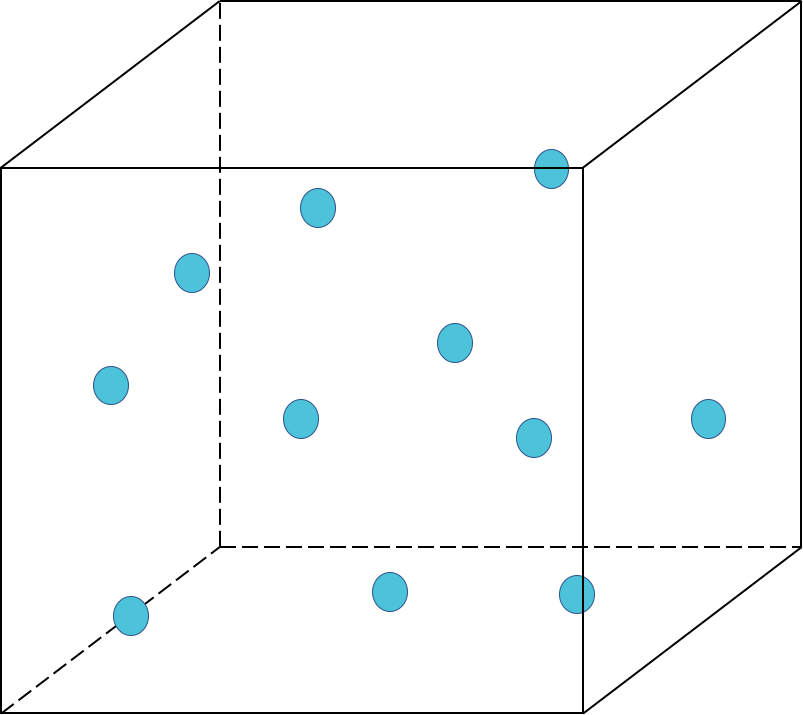
\includegraphics[width=2in]{bubbles_in_cell.png}\\
  \caption{Bubbles dispersed in cell volume.}
  \label{fig:bubbles_in_cell}
\end{figure} 

The number of moles, represented by n, is the summation of all chemical/elemental species in a the bubble. For a system for which we are trying to remove Xenon gas using Helium as our sparging gas, n could be a collection of Helium and Xenon gas. The number of moles in a single bubble is calculated by dividing the total moles of gas in the cell by the number of bubbles. 

 \begin{equation}
 	n_{bubble} = \frac{1}{\# of bubbles} \sum_{j=1}^{k} n_{j}
\end{equation}

The number of bubbles determined from a species transport solve. Because the void faction in the MSRE is so low ($>$1.0 \%) \cite{engel1971}, bubble interactions are neglected. Bubble diameter is solved using the assumption what all bubbles in the cell volume are the same size. 

Two solution methods are employed to solve for bubble diameter. The first involves solving the non-linear Equation \ref{eq:bubble_model} using Newtons Method, which will be discussed later. The second involves making the assumption $P_{b} \approx P_{l}$, this allows for the direct calculation of bubble diameter. 

\begin{equation}
 	D = \bigg(\frac{6nRT_{l}}{\pi P_{l}} \bigg)^{1/3}
	\label{eq:direct_bubble_solve}
\end{equation}

To justify this assumption, the contribution of bubble pressure due to surface tension bust be low. Looking at Equation \ref{eq:young-laplace},  $ 4\sigma_{l}/d \rightarrow \infty$ as $d \rightarrow 0$. As the bubble gets smaller, the contribution from surface tension increases. The range of bubble sizes considered in the MSRE was between $0.0127 - 0.0508$ cm \cite{engel1971}. Figure \ref{fig:pressure_contribution_of_surface_tension} shows the contribution of surface tension to the bubble pressure for a range of bubbles considered in the MSRE. 

\begin{figure}[ht]
  \centering
  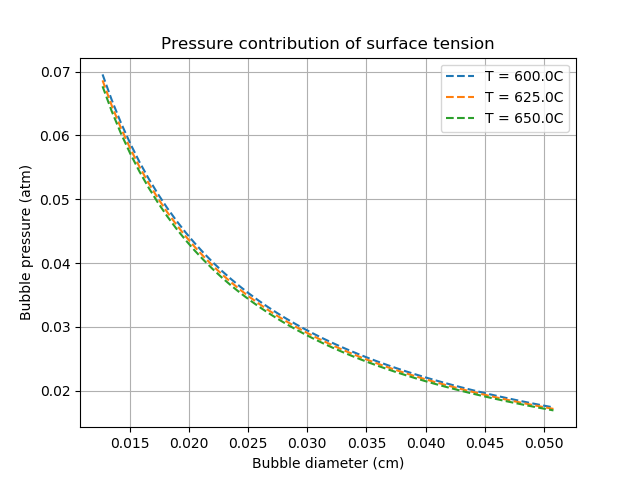
\includegraphics[width=4.5in]{pressure_contribution_of_surface_tension.png}\\
  \caption{Pressure contribution of surface tension.}
  \label{fig:pressure_contribution_of_surface_tension}
\end{figure} 

From Figure \ref{fig:pressure_contribution_of_surface_tension} as expected the contribution from surface tension is highest for smaller bubbles. As temperature increases surface tension slightly decreases leading to a smaller pressure contribution. For a system pressure of 1 and 2 atm, the maximum contribution to the bubble pressure would be 6.54\% and 3.38\% respectively. 

\subsection{Boundary Conditions}\label{ch:bubble_BC}
There are a number of boundary conditions required to solve the interfacial area. These conditions include inlet: temperature, pressure, gas molar flow rate and bubble diameter. Together temperature, pressure, and bubble diameter are utilized in calculating the number of moles in a single bubble by rearranging equation \ref{eq:direct_bubble_solve}. The number of bubbles is calculated by dividing the molar flow rate of gas being injected by the number of moles in a single bubble. 

Gas removal is accomplished by defining a bubble removal efficiency ($S_{eff}$) at the removal location. For gas phase species $i$, the mass flow rate entering the cell is calculated via the flux entering the cell multiplied by the face surface area. The resulting amount of species $i$ exiting the system is then calculated using Equation \ref{eq:vol_removal_term}.













    \chapter{Implementation of Species Transport }\label{ch:implimentation_of_species_transport}

Implementing the generalized multi-phase species transport equation is done on a finite volume mesh. Each cell volume is integrated over and all properties and scalar quantities are assumed to be constant in the cell. Because the entire cell volume is integrated, species concentration are solved for concentration changes in the cell volume and not the phase volume. This treatment requires that volumetric source terms be integrated over the phase volume and not the cell volume to ensure that mass is conserved. 

% Averaging operators
\section{Averaging Operators}
Various methods of averaging exist for converting microscopic conservation equations into macroscopic ones. This technique involves averaging parameters of interest over space, time or both where the spacial variation of concentration is ignored in the cell. CTF is discritized on a finite volume mesh, meaning that volume averaging operators will be needed for species concentration for all phases in the unit cell. Let \textit{V} represent total volume of a cell, \textit{V} can be broken up further into sub domains \textit{$V_{l}$} and \textit{$V_{g}$} where \textit{l} denotes liquid and \textit{g} denotes gas. The volume average of species concentration \textit{C} over the entire volume is shown in Equation \ref{eq:avg_op_over_cell} \cite{kazimi1990}:

\begin{equation}
    \overline{C} = \frac{1}{V}\iiint_{V}CdV
    \label{eq:avg_op_over_cell}
\end{equation}

The concentration can also be averaged over the phase volume \textit{k}:

\begin{equation}
    \overline{C}_{k} = \frac{1}{V_{k}}\iiint_{V_{k}}CdV = \frac{1}{V_{k}}\iiint_{V}\alpha_{k}CdV
    \label{eq:avg_spec_con}
\end{equation}

Where $\alpha_{k}$ is the phase density function; equal to 1 for a point in phase \textit{k} and zero when not. The fraction of cell volume occupied by phase \textit{k} is the void fraction $\overline{\alpha}_{k}$.

\begin{equation}
    \overline{\alpha}_{k} = \frac{1}{V}\iiint_{V}\alpha_{k}dV = \frac{V_{k}}{V}
    \label{eq:avg_void}
\end{equation}

The concentration of species in phase k can also be averaged over the volume occupied by phase k: this value is denoted by $\langle \overline{C}_{k} \rangle_{k}$. 

\begin{equation}
    \langle \overline{C}_{k} \rangle_{k} = \frac{1}{V_{k}}\iiint_{V_{k}}C_{k}dV = \frac{1}{V_{k}}\iiint_{V}\alpha_{k}C_{k}dV
    \label{eq:avg_spec_con_volk}
\end{equation}

Combining Equations \ref{eq:avg_spec_con}, \ref{eq:avg_void} and \ref{eq:avg_spec_con_volk} gives the relations between averaged concentrations.

\begin{equation}
    \overline{C}_{k} = \langle \overline{C}_{k} \rangle_{k}\overline{\alpha}_{k}
\end{equation}

The value $\langle \overline{C}_{k} \rangle_{k}$ represents the species concentration if all of the cell volume was occupied by phase k. $\overline{C}_{k}$ is the species concentration of interest. Multiplying $\overline{C}_{k}$ by \textit{V} returns the amount of species in the cell volume. 

% discretization
\section{Discretization}

%\subsection{Finite volume method}
Species transport utilizes the same discretization method as CTF, finite volume. The data types are further broken down in to scalar and vector (momentum) cells, with these cells overlapping one another shown in Figures \ref{fig:ax_mesh} and \ref{fig:lat_mesh} \cite{salko2017}. 

The averaged operators previously discussed are now applied to Equation \ref{eq:two_phase_species_con_integral_volume}; starting with the conservation of species \textit{i} in phase \textit{k}. 

\begin{equation}
	\iiint_{V} \frac{\partial \alpha_{k}C^{k}_{i} }{\partial t}\,dV = -\iint_S n \cdot F^{k}_{i} \,dS + \iiint_V \alpha_{k}C_{V,i}^{i} \,dV
	\label{eq:start_eq_of_discretization}
\end{equation}
\FloatBarrier
\newpage

\begin{figure}[p]
  \centering
  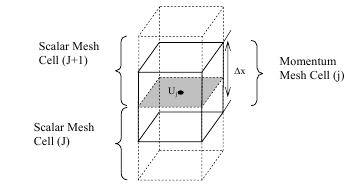
\includegraphics[width=4in]{images/axial_mesh_cells.png}\\
  \caption{Axial meshing.}
  \label{fig:ax_mesh}
\end{figure} 

\begin{figure}[p]
  \centering
  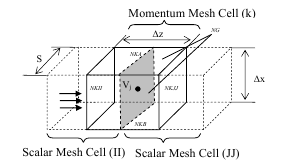
\includegraphics[width=4in]{images/lat_mesh_cells.png}\\
  \caption{Lateral meshing.}
  \label{fig:lat_mesh}
\end{figure} 

\newpage
\FloatBarrier

Starting with Equation \ref{eq:avg_spec_con_volk}, the time variance in equation \ref{eq:start_eq_of_discretization} is averaged over the cell volume to give:

\begin{equation}
    \iiint_{V} \frac{\partial \alpha_{k}C^{k}_{i} }{\partial t}\,dV = \frac{\partial V_{k}\langle \overline{C^{k}}_{i} \rangle_{k}}{\partial t}
\end{equation}

$V_{k}$ however, is $\overline{\alpha}_{k}V$ and $\langle \overline{C^{k}}_{i} \rangle_{k}\overline{\alpha}_{k} = \overline{C^{k}}_{i}$. This same relation is used to evaluate the second term on the left hand-side of Equation \ref{eq:start_eq_of_discretization}. Because the volume of each cell is constant, \textit{V} can be taken out of the time derivative and moved to the right hand side. 

\begin{equation}
    \frac{\partial \overline{C^{k}}_{i}}{\partial t} = - \frac{1}{V}\iint_S n \cdot F^{k}_{i} \,dS + \sum \overline{C^{k}}_{V,i}
    \label{eq:avg_transport_eqn}
\end{equation}

A summation is taken for the volumetric generation term to account for multiple source terms. 

% Upwind flux
\subsection{Upwind Differencing Scheme}
The contribution due to species flux across the cell boundary is modeled using an first order upwind differencing scheme \cite{versteeg2007}. This flux is convection dominate which allows for the removal of the diffusive term. The inner product of the unit normal flux across the face reduces to the velocity across the face multiplied by the species concentration in the neighboring cell or the cell itself, depending upon the flow direction. An example for 2-D flow is shown in Figure \ref{fig:upwind_difference_scheme} for scalar cell (i, j). 

In Figure \ref{fig:upwind_difference_scheme}, flow is going from left to right and bottom to up. When CTF loops over cell (i, j), it loops over all cells connected to calculate the flux across the cell faces. To calculate the inward flux, the velocity at the South and West faces are multiplied by the species concentration in cells (i-1, j) and (i, j-1). The outward flux from cell (i, j) is calculated by multiplying the species concentration is cell (i, j) by the velocity at each face. Because CTF works on a staggered mesh, the velocities at each cell face is defined at that location via the momentum mesh cells. For generalized 3-D flow on a Cartesian rectangular mesh, species flux is represented in Equation \ref{eq:integral_to_flux}.

\FloatBarrier
\newpage

\begin{figure}[p]
  \centering
  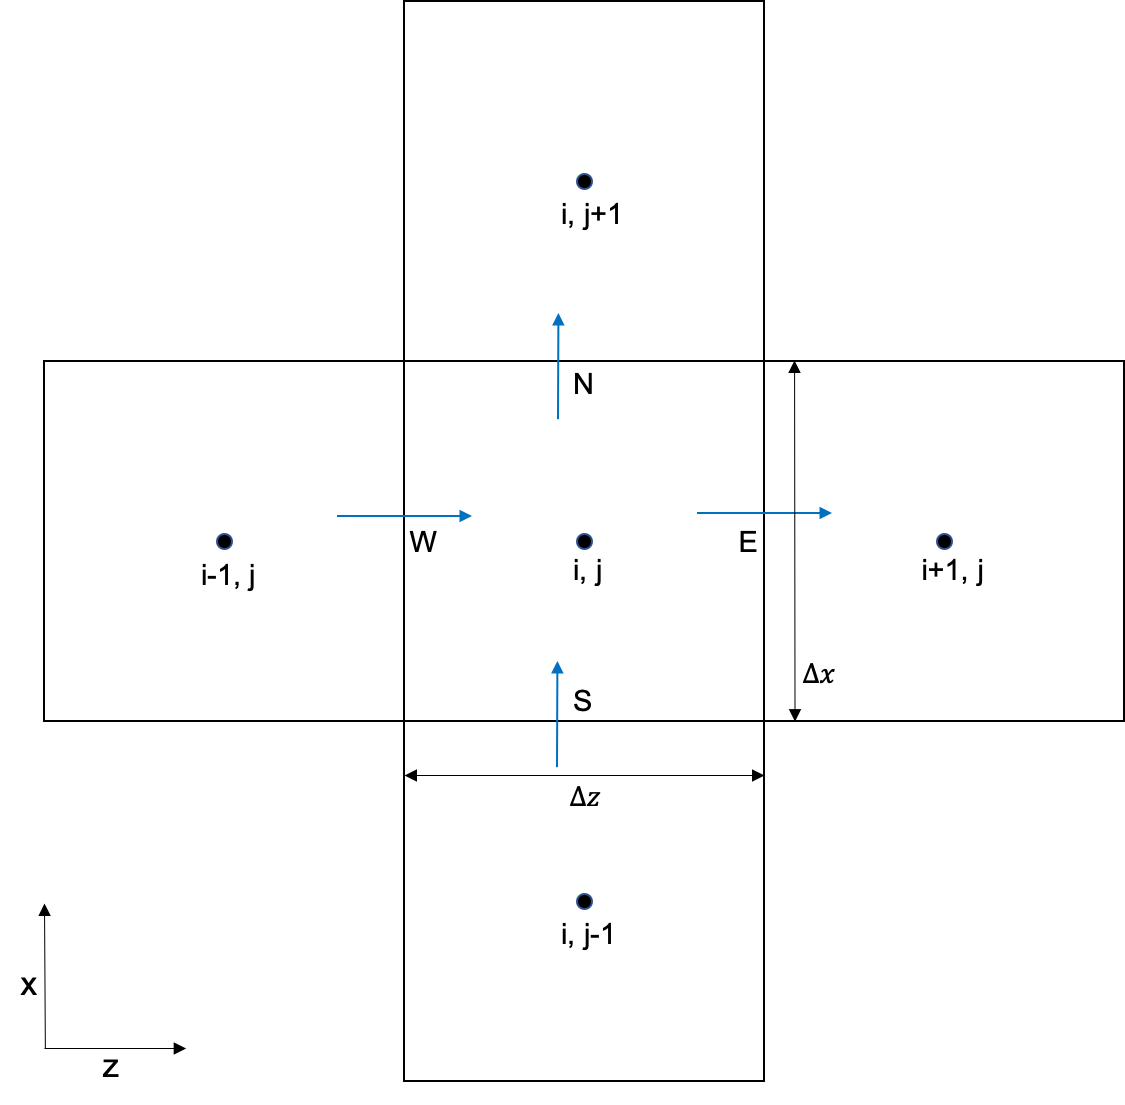
\includegraphics[width=4in]{images/2-DConvection.png}\\
  \caption{2-D Upwind flux}
  \label{fig:upwind_difference_scheme}
\end{figure}

\newpage
\FloatBarrier

\begin{equation}
    \frac{1}{V}\iint_S n \cdot F \,dS = \frac{1}{V}\bigg[ F_{x}A_{x} + F_{y}A_{y} + F_{z}A_{z}\bigg]
    \label{eq:integral_to_flux}
\end{equation}

Looking at Figure \ref{fig:upwind_difference_scheme} let us now define the positive z flow going from left to right, positive x flow going from down to up. Let's now add another dimension $y$, using $k$ index, pointing into the figure making the positive flow direction going into the page. The face coming out of the page is denoted by $O$ and in by $I$. $A_{x}$ becomes $\Delta z \Delta y$, $A_{z}$ becomes $\Delta x \Delta y$, $A_{y}$ becomes $\Delta x \Delta z$ and $V$ becomes $\Delta z \Delta x \Delta y$. If flow is assumed to be going to in the positive direction for each spacial degree of freedom, the flux for each direction is summarized in Table \ref{tab:upwind_flux_eqns}. 

In the case of 3-D flow in the positive direction, Equation \ref{eq:avg_transport_eqn} for a one species in single phase flow becomes:

\begin{equation}
\begin{aligned}
    \frac{\partial \overline{C}}{\partial t} = - \frac{1}{\Delta z \Delta x \Delta y}
     \bigg[ & \big(v_{S} \overline{C}_{i,j-1,k} - v_{N}\overline{C}_{i,j,k}\big)\Delta z \Delta y \\ + 
    & \big(v_{W} \overline{C}_{i-1,j,k} - v_{E}\overline{C}_{i,j,k}\big)\Delta x \Delta z \\ + 
    & \big(v_{O} \overline{C}_{i,j,k-1} - v_{I}\overline{C}_{i,j,k}\big)\Delta x \Delta y \bigg] + \sum \overline{C}_{V}
    \label{eq:avg_transport_eqn_with_flux}
\end{aligned}
\end{equation}

\subsection{Time Marching Scheme}
After discretizing the spacial variables of Equation \ref{eq:avg_transport_eqn}, the variance in time is addressed using two schemes: explicit and implicit Euler methods. For explicit methods, the time dependent solution is updated using information from the previous time step. Implicit methods utilize information on the current time step to solve the PDE. 

\vspace{12.7mm} %5mm vertical space

\begin{table}[htbp!]
   \caption{\label{tab:upwind_flux_eqns} Upwind flux}
   \centering
   \begin{tabular}{l l l}
   \hline
   \textbf{Flux} & \textbf{Positive flow} & \textbf{Negative flow} \\
   \hline 
    $F_{x} \approx$ & $v_{S} C_{i,j-1,k} - v_{N}C_{i,j,k}$ & $v_{N}C_{i,j,k} - v_{S} C_{i,j-1,k}$ \\ [1ex]
    $F_{y} \approx$ & $v_{W} C_{i-1,j,k} - v_{E}C_{i,j,k}$ & $v_{E}C_{i,j,k} - v_{W} C_{i-1,j,k}$ \\ [1ex]
    $F_{z} \approx$ & $v_{O} C_{i,j,k-1} - v_{I}C_{i,j,k}$ & $v_{I}C_{i,j,k} - v_{O} C_{i,j,k-1}$ \\ [1ex]
   \hline
   \end{tabular}
\end{table}

\subsubsection{Explicit Euler}
To derive the first order explicit Euler scheme we will start with Equation \ref{eq:avg_transport_eqn_with_flux} for 1-D flow in the x-direction.

\begin{equation}
        \frac{\partial \overline{C}}{\partial t} = - \frac{1}{\Delta x} \big(v_{S} \overline{C}_{j-1} - v_{N}\overline{C}_{j}\big)  + \sum \overline{C}_{V}
        \label{eq:1-D_x-direction_convection}
\end{equation}

The fundamental theorem of calculus states that the derivative of $\overline{C}(t,x)$ with respect to time is:

\begin{equation}
    \frac{\partial \overline{C}}{\partial t} = \lim_{\Delta t\to 0} \frac{\overline{C}(t+\Delta t, x) - \overline{C}(t,x)}{\Delta t}
    \label{eq:Def_theo_of_calc}
\end{equation}

Equation \ref{eq:Def_theo_of_calc} can be approximated by taking small values of $\Delta t$. Plugging in Equation \ref{eq:Def_theo_of_calc} into equation \ref{eq:1-D_x-direction_convection} and solving for $\overline{C}(t+\Delta t, x)$ gives:

\begin{equation}
    \overline{C}(t+\Delta t, x) = \overline{C}(t,x) - \frac{\Delta t}{\Delta x} \big(v_{S} \overline{C}_{j-1}(t,x) - v_{N}\overline{C}_{j}(t,x)\big)  + \Delta t\sum \overline{C}_{V}(t,x)
    \label{eq:explicit_method}
\end{equation}

% Consider moving this section
%%%%%%%%%%%%%%%%%%%%%%%%%%%%%%%%%%%%%%%%%%%%%%%%%%%%%%%%%%%%%%%%%%%%%%%%%
As previously mentioned, the upwind difference scheme is first order. The first order convergence is shown using a Taylor series expansion \cite{versteeg2007} for a simple 1-D example shown in Figure \ref{fig:1_D_upwind_flux}.

\begin{figure}[ht]
  \centering
  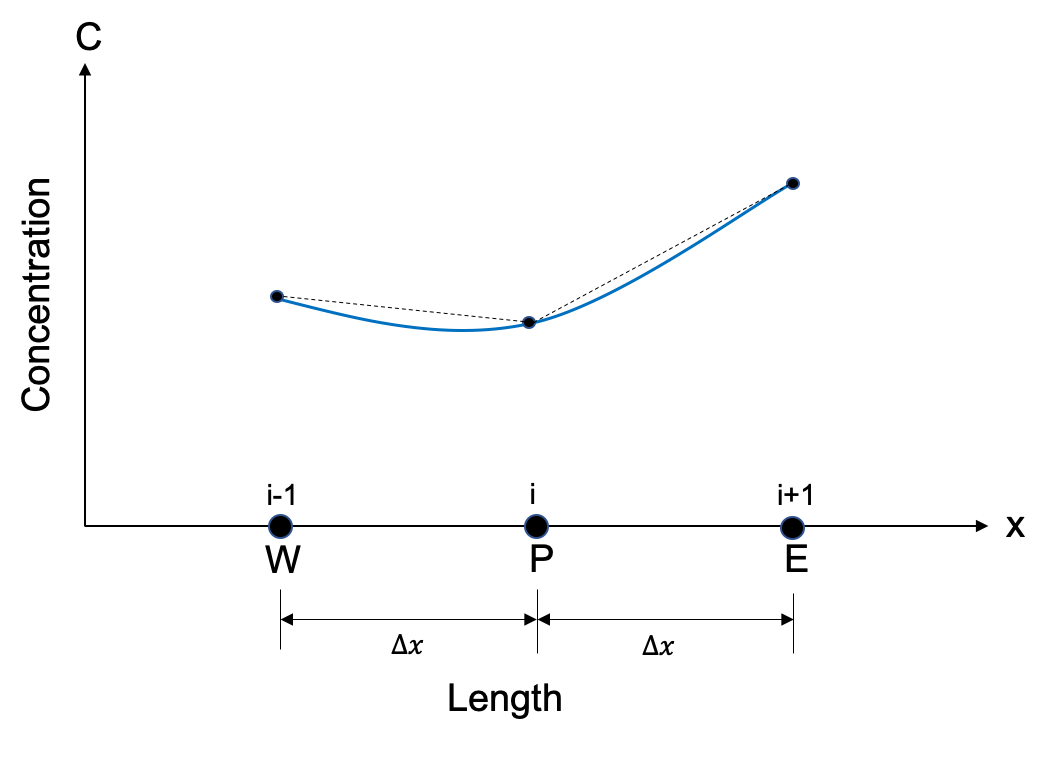
\includegraphics[width=5in]{images/1-DConvection.png}\\
  \caption{1-D Upwind flux}
  \label{fig:1_D_upwind_flux}
\end{figure}

For function $C(x + \Delta x)$ a Taylor series expansion about point $i$ at $x$ is shown in Equation \ref{eq:Taylor_second_order}.

\begin{equation}
    C(x+\Delta x) = C(x) + \bigg(\frac{\partial C}{\partial x}\bigg)_{x}\Delta x + \bigg(\frac{\partial^{2} C}{\partial x^{2}}\bigg)_{x}\frac{\Delta x^{2}}{2} + O(\Delta x^{3})
    \label{eq:Gen_Taylor_second_order}
\end{equation}

The concentration at Point $E$ (i+1) upwind of $P$ (i) is represented by Equation \ref{eq:Gen_Taylor_second_order}.

\begin{equation}
    C_{E} = C_{P} + \bigg(\frac{\partial C}{\partial x}\bigg)_{P}\Delta x + \bigg(\frac{\partial^{2} C}{\partial x^{2}}\bigg)_{P}\frac{\Delta x^{2}}{2} + O(\Delta x^{3})
    \label{eq:Taylor_second_order}
\end{equation}

Solving Equation \ref{eq:Taylor_second_order} for the first derivative gives:

\begin{equation}
    \bigg(\frac{\partial C}{\partial x}\bigg)_{P} = \frac{C_{E} - C_{P}}{\Delta x} - \bigg(\frac{\partial^{2} C}{\partial x^{2}}\bigg)_{P}\frac{\Delta x}{2} + ...
    \label{eq:Taylor_series_updwind_flux_order}
\end{equation}

Equation \ref{eq:Taylor_series_updwind_flux_order} shows that the derivative at point $P$ can be approximated by Equation \ref{eq:upwind_flux_approx} by truncating the higher order terms. 

\begin{equation}
    \bigg(\frac{\partial C}{\partial x}\bigg)_{P} \approx \frac{C_{E} - C_{P}}{\Delta x}
    \label{eq:upwind_flux_approx}
\end{equation}

The error involved in approximating the derivative is proportional to the size of $\Delta x$. This implies that the error in Equation \ref{eq:upwind_flux_approx} can be reduced by decreasing $\Delta x$ \cite{versteeg2007}. The rate at which the error approaches zero is then proportional to $\Delta x$ to the first power, making the scheme first order in space. 

For an implicit solution terms in Equation \ref{eq:explicit_method} are taken from the current time step.

\begin{equation}
    \overline{C}(t+\Delta t, x) = \overline{C}(t,x) - \frac{\Delta t}{\Delta x} \big(v_{S} \overline{C}_{j-1}(t+\Delta t,x) - v_{N}\overline{C}_{j}(t+\Delta t,x)\big)  + \Delta t\sum \overline{C}_{V}(t+\Delta t,x)
    \label{eq:implicit_method}
\end{equation}

The solution to Equation \ref{eq:implicit_method} is accomplished by solving a set of linear algebraic equations. 
%%%%%%%%%%%%%%%%%%%%%%%%%%%%%%%%%%%%%%%%%%%%%%%%%%%%%%%%%%%%%%%%%%%%%%%%%


    \chapter{Results} \label{ch:Results}
Throughout the course of this study a number of unit tests and case studies were preformed to assess codes capability and performance. These test are broken down into three categories: generalized species transport, mult-phase transport and MSR sample problems. Many of the test involve the use of a coupled xenon iodine sample problem shown in Equations \ref{eq:XenonGeneralDiffEq} and \ref{eq:IodineGeneralDiffEq}.

\begin{equation}
    \frac{\partial \rho_{Xe}}{\partial t} = -\nabla (\rho_{Xe}v) + \frac{M_{Xe}}{N_{A} (1-\alpha)} \gamma_{Xe}\Sigma_{f}\Phi + \frac{M_{Xe}}{M_{I}}\lambda_{I}\rho_{I} - \lambda_{Xe}\rho_{Xe} - \sigma_{a}\Phi\rho_{Xe}
    \label{eq:XenonGeneralDiffEq}
\end{equation}

\begin{equation}
    \frac{\partial \rho_{I}}{\partial t} = -\nabla (\rho_{I}v) + \frac{M_{I}}{N_{A}(1-\alpha)} \gamma_{I}\Sigma_{f}\Phi - \lambda_{I}\rho_{I}
    \label{eq:IodineGeneralDiffEq}
\end{equation}

In this problem, ${}^{135}Xe$ and ${}^{135}I$ are born under a neutron flux with each undergoing fluctuations based their own individual source terms. Because source terms for nuclear interactions are assessed with atomic number density, these terms must be converted to mass density. Starting from the left hand side of Equation \ref{eq:XenonGeneralDiffEq}, the first term is change due to transport followed by source from fission, decay of ${}^{135}I$, decay of ${}^{135}Xe$, and transmutation. In Equation \ref{eq:IodineGeneralDiffEq} the first term on the right hand side is transport followed by generation from fission and decay of ${}^{135}I$. Table \ref{tab:Test_parameters} shows the parameters utilized in testing. 

\begin{table}[htbp!]
   \caption{\label{tab:Test_parameters} Test problem parameters}
   \centering
   \begin{tabular}{lll}
   \hline
   \textbf{Parameter} & \textbf{Value} & \textbf{Unit} \\
   \hline 
   $\gamma_{I}$ & $6.3033$ \cite{cole2019} & \% \\ [1ex]
   $\gamma_{Xe}$ & $0.2468$ \cite{cole2019} & \% \\ [1ex]
   $\Sigma_{f}$ & 9.7532E-1 \cite{cole2019} & 1/ft \\ [1ex]
   $\Phi$ & 2.5E16 \cite{nestor1960} &  n/ft${}^{2}$/s \\ [1ex]
   $\lambda_{Xe}$ & 2.11E-5 \cite{cole2019} & 1/s\\ [1ex]
   $\lambda_{I}$ & 2.9306E-5 \cite{cole2019} & 1/s  \\ [1ex]
   $M_{Xe}$ & 135.0 & lbm/mol\\ [1ex]
   $M_{I}$ & 135.0 & lbm/mol \\ [1ex]
   $N_{A}$ & 6.0221409E23 & atoms/mol \\ [1ex] 
   $\alpha$ Void Fraction & - & - \\ [1ex]
   \hline
   \end{tabular}
\end{table}

Some cases depict convergence using the following global error. I is the number of axial levels and J is the number of channels.

\begin{equation}
    \text{GlobalError} = \bigg(\frac{\sum (C_{exact}-C_{approx})^{2}}{IJ}\bigg)^{1/2}
\end{equation}


\section{General Species Transport}\label{sec:gen_transport}
Generalized transport consist of four main tests, three of which test individual components of the transport equation while the last test integrated effects. The individual components tested are volumetric source terms, axial driven transport and lateral driven transport. 

% Source term test
\subsection{Source Term}
The problem consist of a single channel with 10 levels. Advection is turned of in the transport equation so that only the source plays a part in the solution. Because of this, the mass averaged velocities aren't required and the problem is left in atomic number density form. In the problem we are checking to make sure that the source method inside of the transported species class is working properly. For this case, we look at the number density, as a function of time, for both ${}^{135}Xe$ and ${}^{135}I$. 

\begin{equation}
    \frac{\partial N_{Xe}}{\partial t} = \gamma_{Xe}\Sigma_{f}\Phi + \lambda_{I}N_{I} - \lambda_{Xe}N_{Xe} - \sigma_{a}\Phi N_{Xe}
    \label{eq:XenonGeneralDiffEqSource}
\end{equation}

\begin{equation}
    \frac{\partial N_{I}}{\partial t} = \gamma_{I}\Sigma_{f}\Phi - \lambda_{I}N_{I}
    \label{eq:IodineGeneralDiffEqSource}
\end{equation}

\begin{equation}
\begin{split}
   N_{Xe}(t)  =\frac{\gamma_{Xe}\Sigma_{f}\phi}{\lambda_{Xe} + 
   \sigma_{a}\phi} + \frac{\gamma_{I}\Sigma_{f}\phi}{\lambda_{Xe} + 
   \sigma_{a}\phi} - \frac{\gamma_{I}\Sigma_{f}\phi}{\lambda_{Xe} - 
   \lambda_{Xe} + \sigma_{a}\phi}e^{-\lambda_{I}t} \\
   - \left[\frac{\gamma_{I}\Sigma_{f}\phi}{\lambda_{Xe} - \lambda_{Xe} +
   \sigma_{a}\phi} + \frac{\gamma_{I}\Sigma_{f}\phi + \gamma_{Xe}\Sigma_{f}\phi}{\lambda_{Xe} + 
   \sigma_{a}\phi} \right]e^{-(\lambda_{Xe} + \sigma_{a}\phi)t}
\end{split}
\end{equation}

\begin{equation}
   N_{I}(t)  =\frac{\gamma_{I}\Sigma_{f}}{\lambda_{I}} \left[1 - e^{-\lambda_{I}t} \right]
   \label{eq:number_density_iodine_time}
\end{equation}

The Xenon and Iodine system were ran for 250000 seconds allowing for build up of both. Three time steps were chosen to demonstrate convergence in each case. Figure \ref{fig:Xe_I_buildup_source_problem} shows the build up from the smallest time step chosen, dt = 10 seconds. Figures \ref{fig:I_error_source_term}, \ref{fig:Xe_error_source_term} show the global error for three time steps; 10s 100s and 1000s. 

\vspace{12.7mm} %5mm vertical space

\begin{figure}[ht]
  \centering
  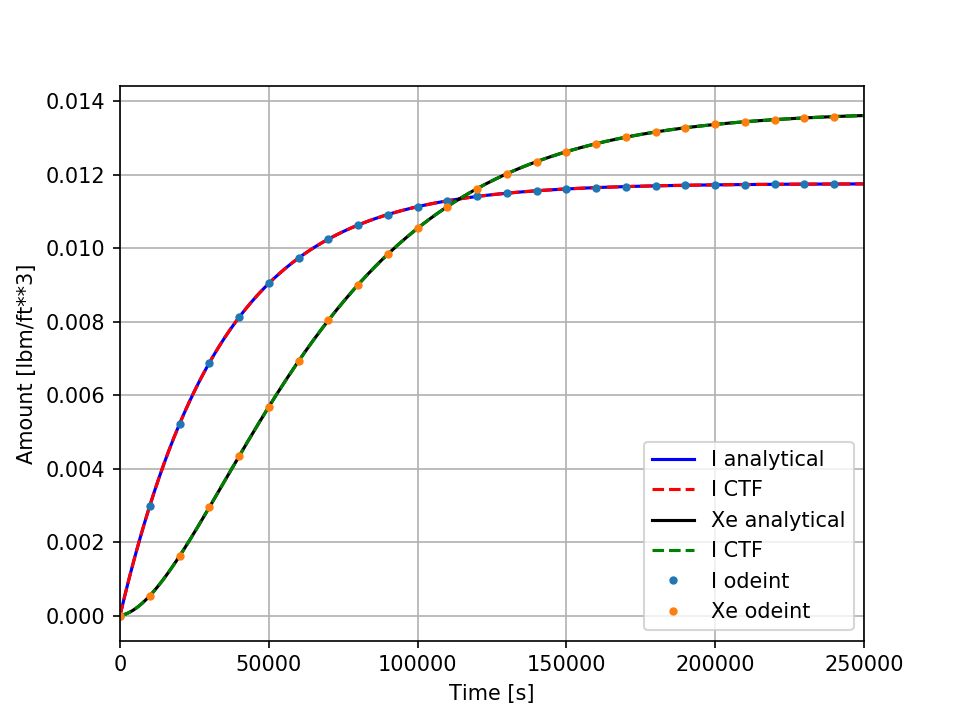
\includegraphics[width=5in]{images/XeIBuildup.png}\\
  \caption{Xe and I build up}
  \label{fig:Xe_I_buildup_source_problem}
\end{figure}

\begin{figure}[ht] 
\centering
\begin{minipage}{.5\textwidth}
  \centering
  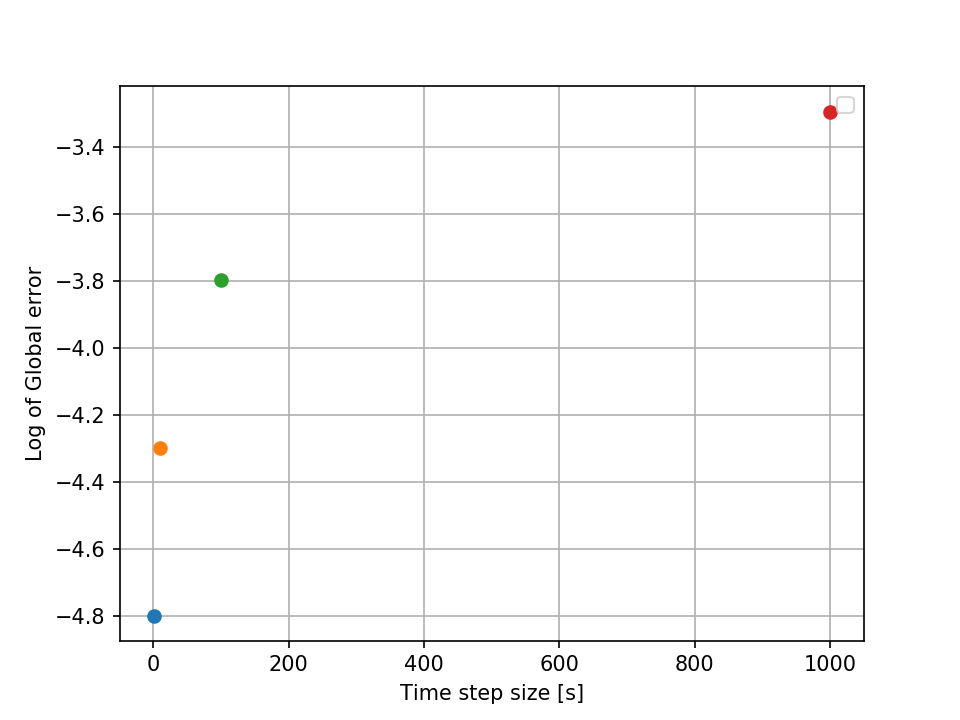
\includegraphics[width=.9\linewidth]{images/IError.png}
  \captionof{figure}{Iodine error}
  \label{fig:I_error_source_term}
\end{minipage}%
\begin{minipage}{.5\textwidth}
  \centering
  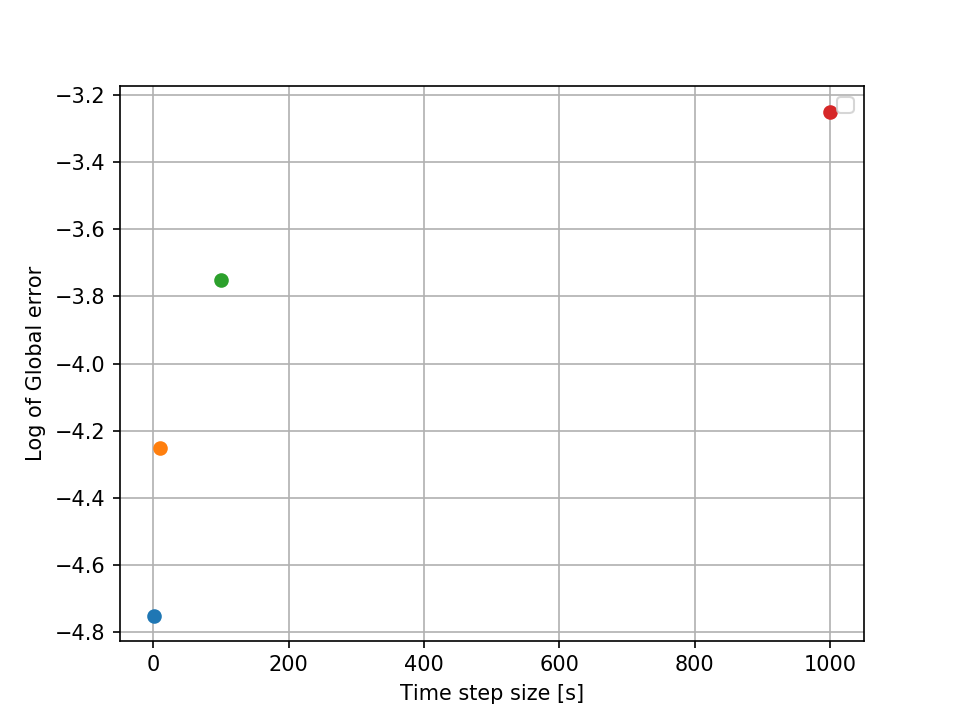
\includegraphics[width=.9\linewidth]{images/XeError.png}
  \captionof{figure}{Xenon error}
  \label{fig:Xe_error_source_term}
\end{minipage}
\end{figure}

Figure \ref{fig:Xe_I_buildup_source_problem} shows three different solutions; analytical, CTF and odeint. We have already discussed the analytical and CTF solutions, the odeint solution comes from the Python module Scipy and is a general ODE solver. All three solutions show good accordance with one another. From Figures \ref{fig:I_error_source_term} \ref{fig:Xe_error_source_term} you can see the global error decreases with decreasing time step size. 

% Single Channel Axial Step change
\subsection{Single Channel Axial Step Change}
This problem consist of a single 1 meter long channel with a varying number of axial levels. There are no source terms in the channel, only advection in the x direction. Initially the inlet concentration is set to 50 with a step change occurring for time greater then 5 seconds. A summary of the problem is shown in Equation \ref{eq:axial_step_change}.

\begin{equation}
\frac{\partial C}{\partial t} = -v_{z} \frac{\partial C}{\partial z} \quad \quad C_{o} = \begin{cases}
5 &  5 > t > 0\\
10 & 5 \geq t
\end{cases}
\label{eq:axial_step_change}
\end{equation}

Figure \ref{fig:axial_step_change} shows the concentration at the outlet of the pipe for three axial meshes. The orange line is the analytical concentration at the outlet of the pipe based on the fluid velocity. For large dx values, the tails on the left and right hand side of the orange line are indicative of numerical diffusion \cite{versteeg2007}. Decreasing the axial meshing size leads to a better approximation to the solution and reduces the error cause by numerical diffusion. 

% Lateral flow step change
\subsection{Multi-channel Lateral Flow Step Change}
Lateral flow is tested in a similar manor to the axial step change test. The only difference is that channels must be stacked next to one another to build the geometry. Instead of being able to change the number of axial levels in a single channel, we must change the number of channel in the problem itself and to change the geometry of each channel as the values of dz become smaller. 

Figure \ref{fig:latFlowResults} shows the outlet concentration. The results mimic the axial flow results, showing numerical diffusion decreases as the lateral meshing gets smaller. 

% Single channel non-constant neutron flux
\subsection{Single Channel Axial Neutron Flux}
The purpose of this problem is to test advective mass transport inside CTF with nonuniform neutron flux. This problem 
consist of a single channel with 100 levels. A neutron flux represented by Equation \ref{eq:variable_neutron_flux}.

\begin{align}
   \phi = \phi_{\theta}\sin\left(\frac{\pi z}{z_{max}}\right)
   & \label{eq:variable_neutron_flux}
\end{align}

\vspace{12.7mm} %5mm vertical space

\begin{figure}[ht] 
\centering
\begin{minipage}{.5\textwidth}
  \centering
  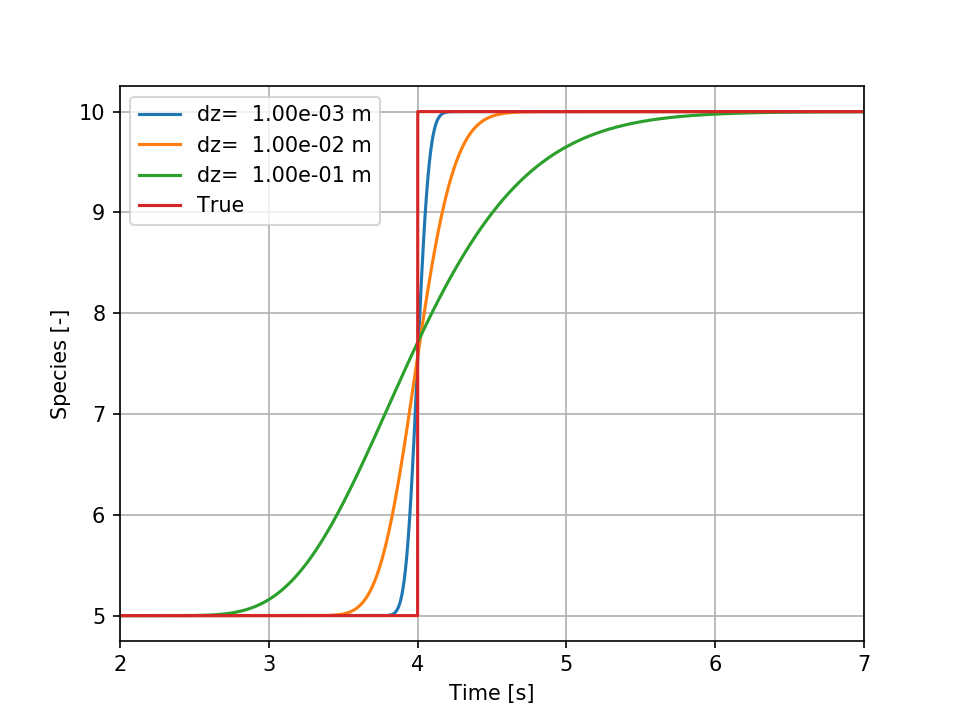
\includegraphics[width=.9\linewidth]{images/transportSpeciesLateral.png}
  \captionof{figure}{Outlet concentration as \\ a function of time for lateral flow}
  \label{fig:latFlowResults}
\end{minipage}%
\begin{minipage}{.5\textwidth}
  \centering
  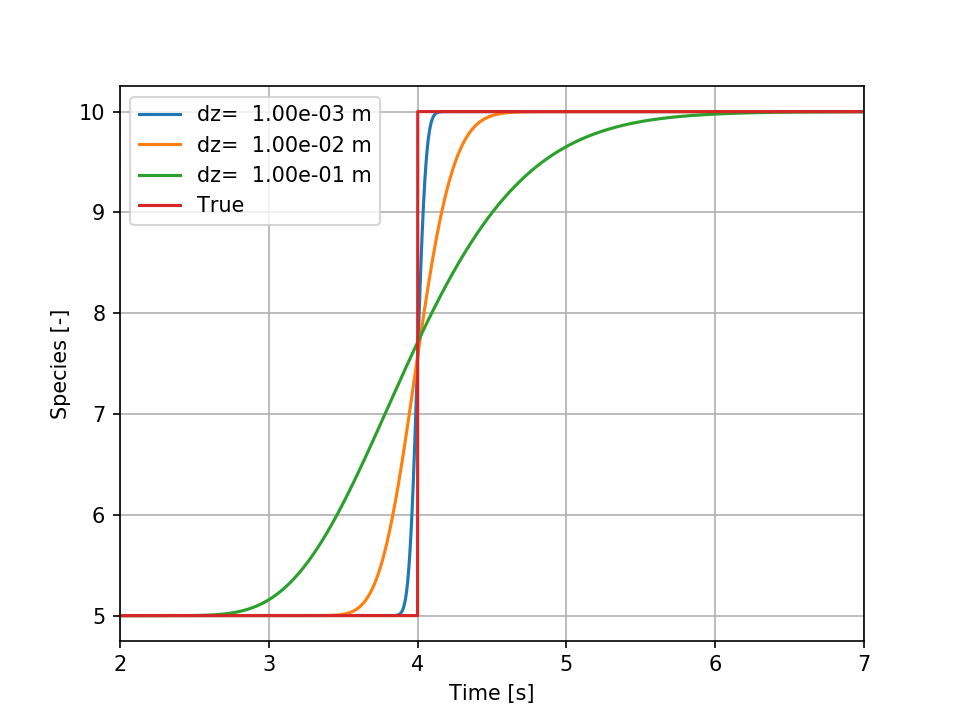
\includegraphics[width=.9\linewidth]{images/transportSpeciesConvection.png}
  \captionof{figure}{Outlet concentration as \\ a function of time for axial flow}
  \label{fig:axial_step_change}
\end{minipage}
\end{figure}

\newpage



In Equation \ref{eq:variable_neutron_flux} $\phi_{\theta}$ is the weighing factor and sets the maximum value at the 
midpoint in the problem. Z is the end point value for each axial level going up the channel and $z_{max}$ is the total 
length of the channel. A flux array is generated inside of the unit test driver and is called to set the flux at each level in 
the problem. The mean value theorem is implemented when generating this array. This is done to accurately represent 
the flux for each axial level as an average value which equals the flux over the integrated area. Equation 
\ref{eq:variable_neutron_flux_mean_value} represents the equation utilized in CTF to build the flux array. 

\begin{align}
   \phi = \left(\frac{1}{z_{2} - z_{1}}\right)\frac{\pi z \phi_{\theta}}{z_{max}}\left[\cos\left(\frac{\pi z_{1}}{z_{max}}\right) - \cos\left(\frac{\pi z_{1}}{z_{max}}\right)\right]
\label{eq:variable_neutron_flux_mean_value}
\end{align}

In Equation \ref{eq:variable_neutron_flux_mean_value} $z_{1}$ and $z_{2}$ represent the bottom and top value for the 
axial level of integration. 

For this case, we look at the transport of ${}^{135}I$ governed by Equation \ref{eq:IodineGeneralDiffEq} for steady state 1-D flow at constant velocity (v).

\begin{equation}
    \frac{d\rho_{I}}{dz} = \frac{1}{v_{z}}\bigg[\frac{M_{I}\gamma_{I}\Sigma_{f}\phi_{\theta}}{N_{A}}\sin\left(\frac{\pi z}{z_{max}}\right) - \lambda_{I}\rho_{I}\bigg]
    \label{eq:Iodine1D}
\end{equation}

The analytical solution is:

\begin{equation}
    \rho_{I}(z) = \frac{M_{I}\pi\gamma_{I}\Sigma_{f}\phi_{\theta}}{z_{max} v Na  A}e^{-\frac{\lambda_{I}z}{v}} - \frac{M_{I}\gamma_{I}\Sigma_{f}\phi_{\theta}}{ v Na  A}\bigg[ \frac{\pi}{z_{max}}\cos{\left(\frac{\pi z}{z_{max}}\right)}-\frac{\lambda_{I}}{v}\sin{\left(\frac{\pi z}{z_{max}}\right)}\bigg]
\end{equation}

\begin{equation*}
    A = \frac{\lambda_{I}^{2}}{v^{2}} + \frac{\pi^{2}}{z_{max}^{2}}
\end{equation*}

Figure \ref{fig:iodine_flux_solution} shows the analytical vs. CTF solution for a system of 100 axial levels. Figure \ref{fig:iodine_flux_error} gives the log of the global error vs. the dz step size. 

\begin{figure}[ht] 
\centering
\begin{minipage}{.5\textwidth}
  \centering
  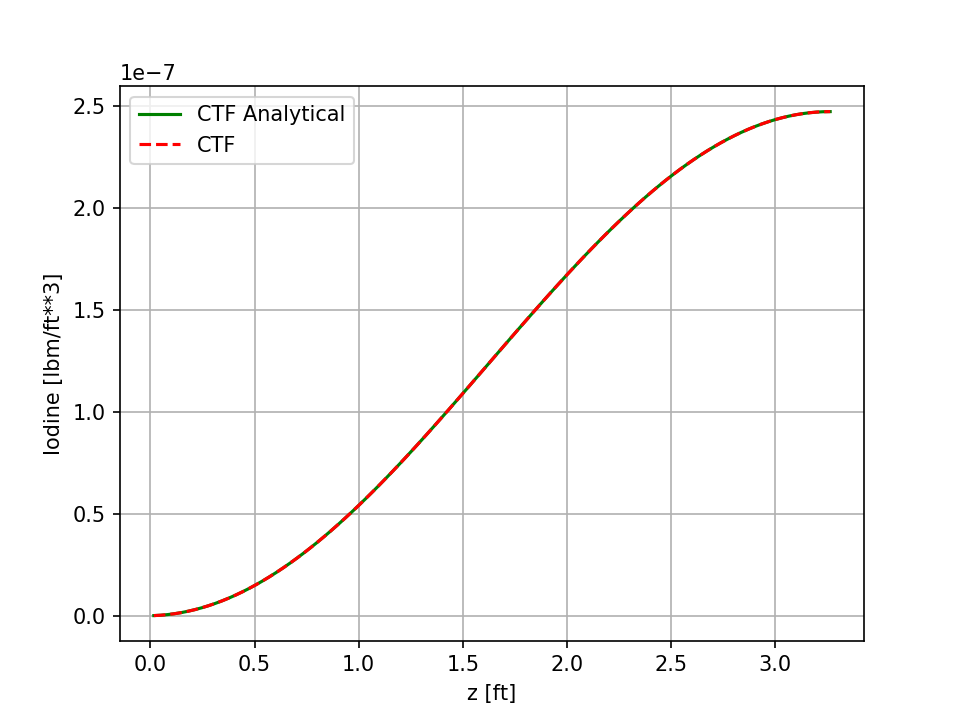
\includegraphics[width=.9\linewidth]{images/transportedSpeciesAxialNonuniform.png}
  \captionof{figure}{Iodine solution}
  \label{fig:iodine_flux_solution}
\end{minipage}%
\begin{minipage}{.5\textwidth}
  \centering
  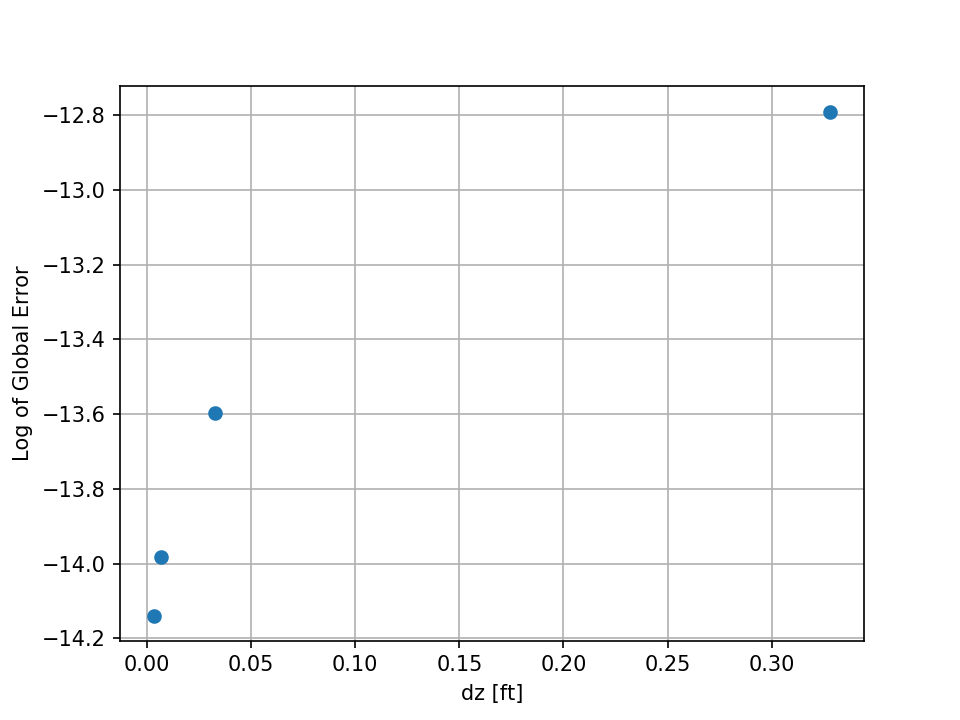
\includegraphics[width=.9\linewidth]{images/transportedSpeciesAxialNonuniformError.png}
  \captionof{figure}{Global error}
  \label{fig:iodine_flux_error}
\end{minipage}
\end{figure}

\newpage

% multiphase species transport
\section{Multi-phase Species Transport}\label{sec:gas_transport}

\subsection{Bubble Growth}
Bubble growth is governed by changes in temperature, pressure and mass. Equation \ref{eq:ideal_gas_law_volume} shows the relation between volume, temperature, pressure and mass. 

\begin{equation}
	V = \frac{nRT}{P}
	\label{eq:ideal_gas_law_volume}
\end{equation}

Volume is directly proportional to moles (n) and temperature (T) and inversely proportional to pressure (P). This means that increasing moles or temperature will cause a direct increase in volume. Increasing the pressure will decrease the bubble volume, leading to an overall decrease in interfacial area. The following cases test this relationship to ensure an accurate representation of bubble dynamics. 

In each of the following test a single 10 level channel is used to determine each variables impact on interfacial area and bubble diameter. The specified variable linearly increases as the species flow up the channel. At the end of the channel, the interfacial area and bubble diameter will be accessed to determine if it increased or decreased. An analytical solution will not be addressed, only the general trend. 

% Temperature effect
\subsubsection{Temperature}
Temperature linearly increases up the channel, bubble diameter and interfacial area are shown in Figures \ref{fig:temp_increase_bubDia} and \ref{fig:temp_increase_intArea}. Figures \ref{fig:temp_decrease_bubDia} and \ref{fig:temp_decrease_intArea} demonstrate the effect of a temperature decrease.

%Pressure effect
\subsubsection{Pressure}
Figures \ref{fig:press_increase_bubDia} and \ref{fig:press_increase_intArea} show bubble diameter and interfacial area under a pressure increase. Figures \ref{fig:press_decrease_bubDia} and \ref{fig:press_decrease_intArea} show a the same variables under and pressure decrease.

\subsubsection{Mass}
Testing masses effect was a little different than temperature and pressure. In the previous two cases mass transfer into or out of the bubble was stopped by setting the mass transfer coefficient (k) to zero. K is set to a small positive value to simulate mass leaving the bubbles. Mass entering the bubbles is achieved by switching the sign of k. A small k value is need to ensure that equilibrium isn't reached between the liquid and gas phase. This will cause bubble diameter and interfacial area to continuously increase or decrease up the channel. Figures \ref{fig:mass_increase_bubDia} through \ref{fig:mass_decrease_intArea} exhibit mass transfer from the bubbles.

\subsection{Interfacial Area Source}
Phase migration is testing in a single channel with two chemical species helium and xenon. At the bottom of the channel helium bubbles at reference diameter $(D_{ref})$ are inject along with xenon dissolved in the liquid phase. As the mixture travels up the channel xenon migrates into the helium bubbles with both streams exiting at the top of the channel. Xenon migration is governed by Equation \ref{eq:liq_side_coupling} where the value for $k$ is taken from \cite{houtzeel1967}. Helium is not allowed to dissolve in the salt by making its mass transfer coefficient zero. Table \ref{tab:intArea_test_parameters} summarizes important parameters utilized in the test.  

\FloatBarrier
\newpage

\begin{figure}[p] 
\centering
\begin{minipage}{.5\textwidth}
  \centering
  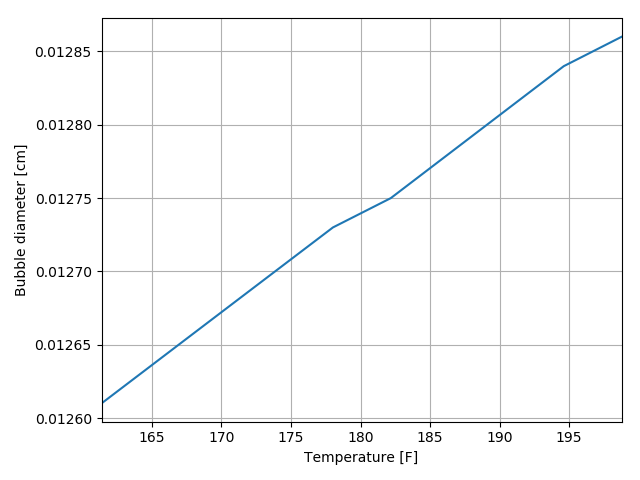
\includegraphics[width=.9\linewidth]{images/BubbleDiaTemperatureIncrease.png}
  \captionof{figure}{effect of temperature increase \\ on bubble diameter}
  \label{fig:temp_increase_bubDia}
\end{minipage}%
\begin{minipage}{.5\textwidth}
  \centering
  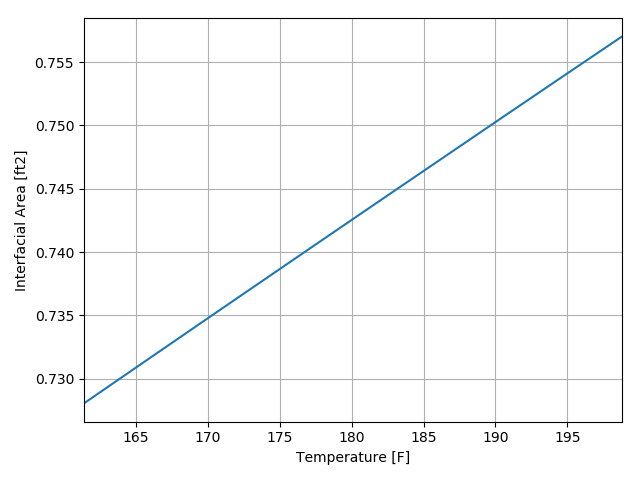
\includegraphics[width=.9\linewidth]{images/IntAreaTemperatureIncrease.png}
  \captionof{figure}{Effect of temperature increase \\ on interfacial area}
  \label{fig:temp_increase_intArea}
\end{minipage}
\end{figure}

\begin{figure}[p] 
\centering
\begin{minipage}{.5\textwidth}
  \centering
  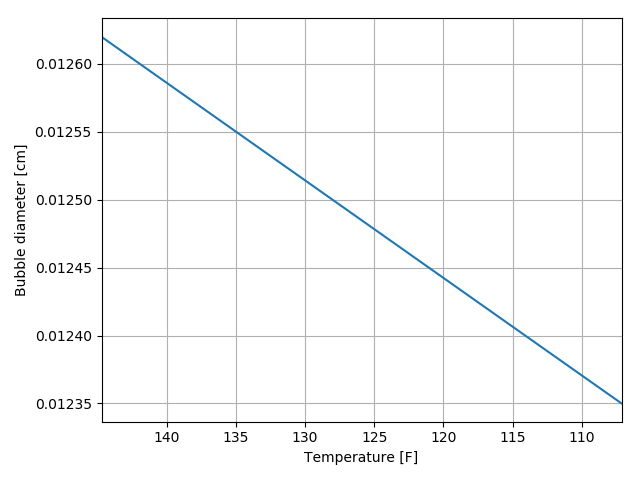
\includegraphics[width=.9\linewidth]{images/BubbleDiaTemperatureDecrease.png}
  \captionof{figure}{Effect of temperature \\ decrease  on bubble diameter}
  \label{fig:temp_decrease_bubDia}
\end{minipage}%
\begin{minipage}{.5\textwidth}
  \centering
  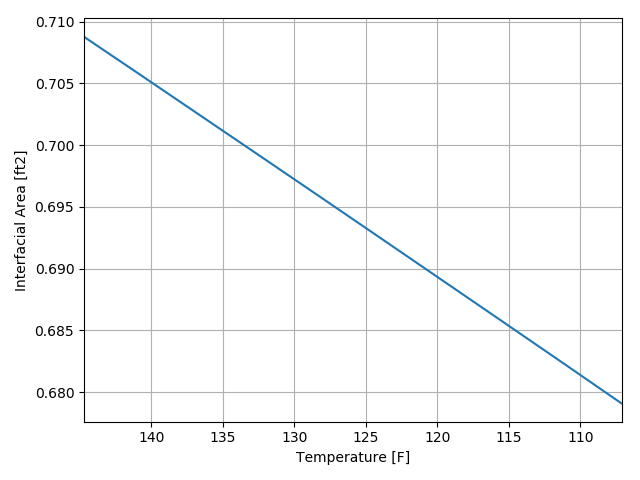
\includegraphics[width=.9\linewidth]{images/IntAreaTemperatureDecrease.png}
  \captionof{figure}{Effect of temperature \\ decrease on interfacial area}
  \label{fig:temp_decrease_intArea}
\end{minipage}
\end{figure}

\FloatBarrier
\newpage
\FloatBarrier

\begin{figure}[p] 
\centering
\begin{minipage}{.5\textwidth}
  \centering
  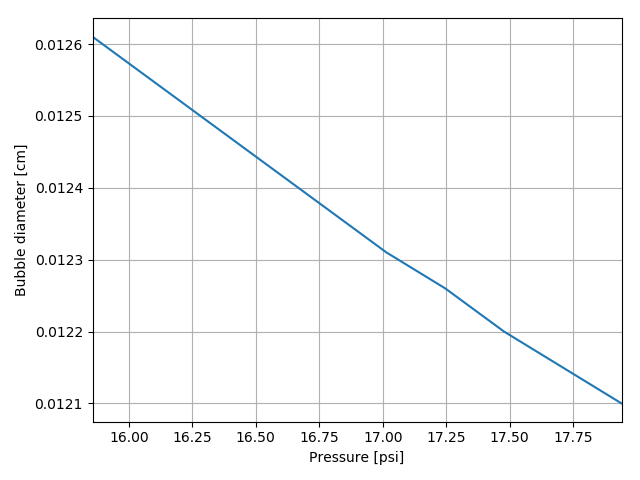
\includegraphics[width=.9\linewidth]{images/BubbleDiaPressureIncrease.png}
  \captionof{figure}{Effect of pressure increase \\ on bubble diameter}
  \label{fig:press_increase_bubDia}
\end{minipage}%
\begin{minipage}{.5\textwidth}
  \centering
  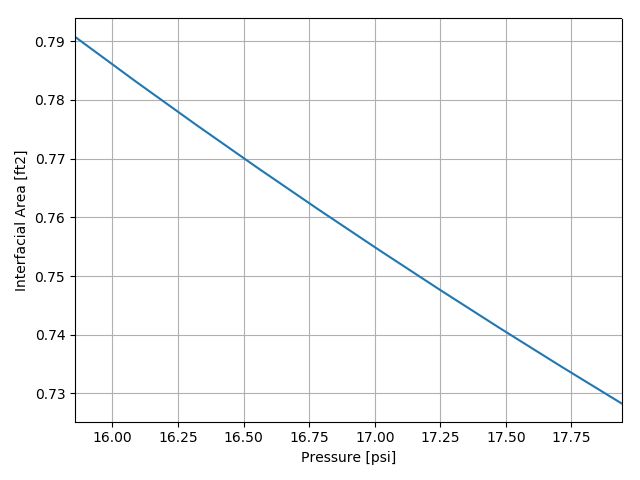
\includegraphics[width=.9\linewidth]{images/IntAreaPressureIncrease.png}
  \captionof{figure}{Effect of pressure increase \\ on interfacial area}
  \label{fig:press_increase_intArea}
\end{minipage}
\end{figure}

\begin{figure}[p] 
\centering
\begin{minipage}{.5\textwidth}
  \centering
  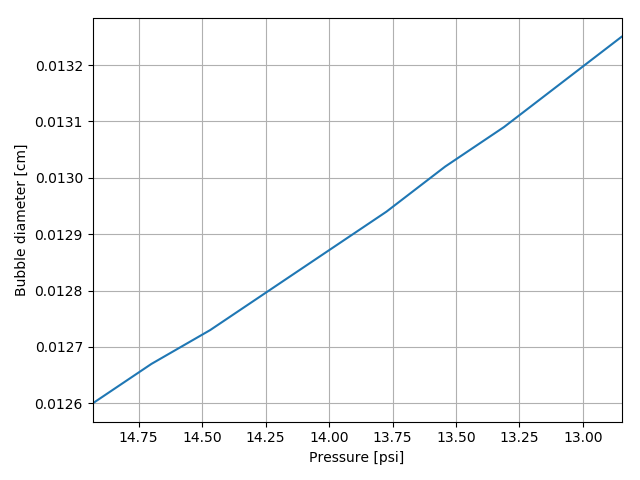
\includegraphics[width=.9\linewidth]{images/BubbleDiaPressureDecrease.png}
  \captionof{figure}{Effect of pressure decrease \\ on bubble diameter}
  \label{fig:press_decrease_bubDia}
\end{minipage}%
\begin{minipage}{.5\textwidth}
  \centering
  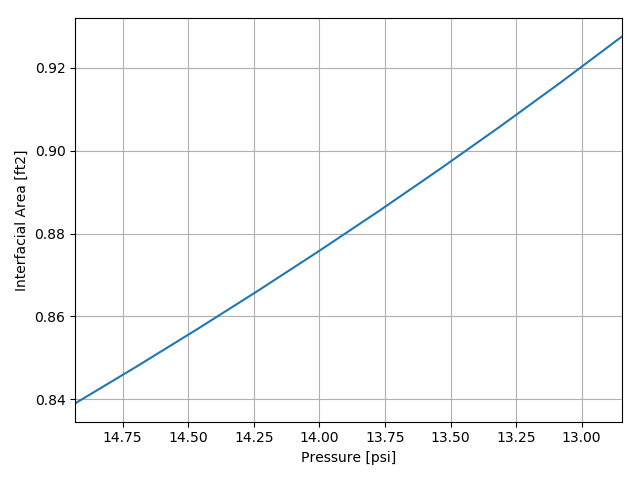
\includegraphics[width=.9\linewidth]{images/IntAreaPressureDecrease.png}
  \captionof{figure}{Effect of pressure decrease \\ on interfacial area}
  \label{fig:press_decrease_intArea}
\end{minipage}
\end{figure}

\FloatBarrier
\newpage
\FloatBarrier



\begin{figure}[p] 
\centering
\begin{minipage}{.5\textwidth}
  \centering
  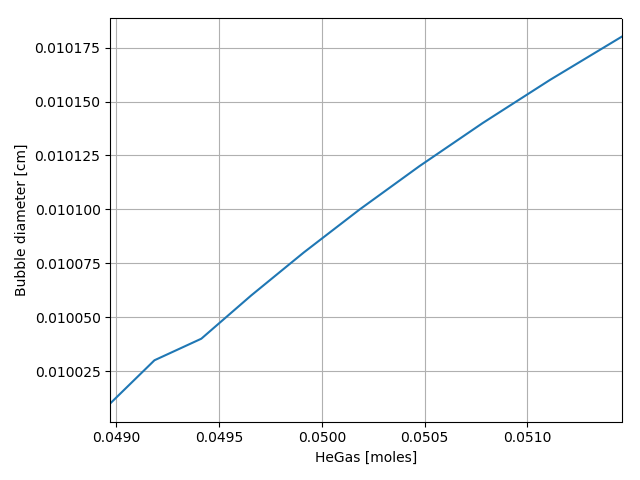
\includegraphics[width=.9\linewidth]{images/BubbleDiaMassIncrease.png}
  \captionof{figure}{Effect of mass increase \\ on bubble diameter}
  \label{fig:mass_increase_bubDia}
\end{minipage}%
\begin{minipage}{.5\textwidth}
  \centering
  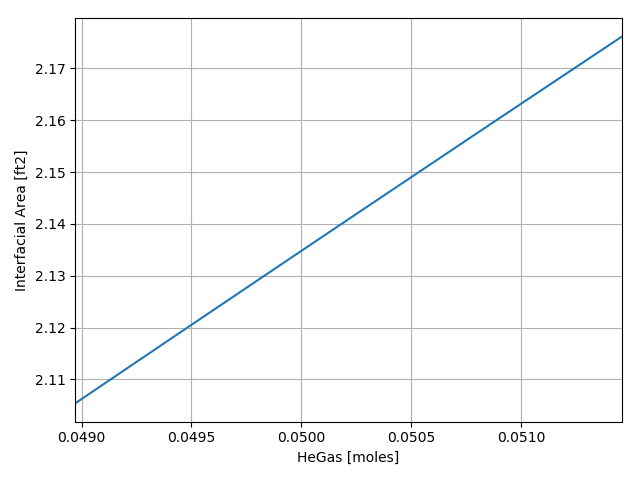
\includegraphics[width=.9\linewidth]{images/IntAreaMassIncrease.png}
  \captionof{figure}{Effect of mass increase \\ on interfacial area}
  \label{fig:mass_increase_intArea}
\end{minipage}
\end{figure}

\begin{figure}[p] 
\centering
\begin{minipage}{.5\textwidth}
  \centering
  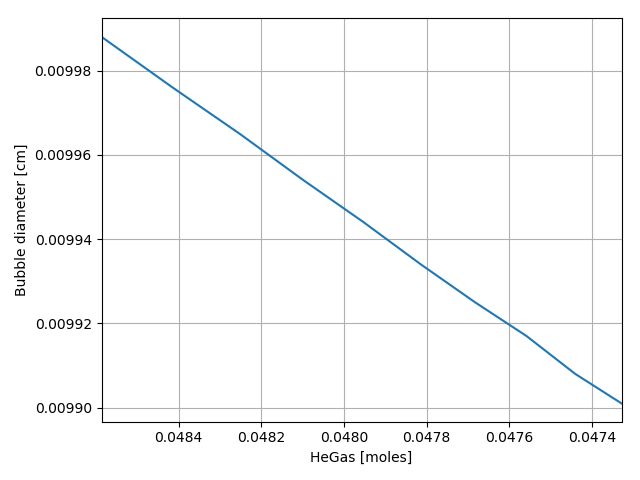
\includegraphics[width=.9\linewidth]{images/BubbleDiaMassDecrease.png}
  \captionof{figure}{Effect of mass decrease \\ on bubble diameter}
  \label{fig:mass_decrease_bubDia}
\end{minipage}%
\begin{minipage}{.5\textwidth}
  \centering
  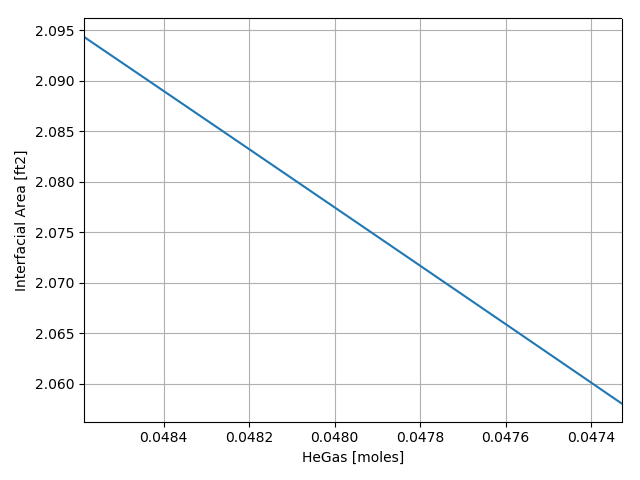
\includegraphics[width=.9\linewidth]{images/IntAreaMassDecrease.png}
  \captionof{figure}{Effect of mass decrease \\ on interfacial area}
  \label{fig:mass_decrease_intArea}
\end{minipage}
\end{figure}

\FloatBarrier
\newpage
\FloatBarrier



\begin{table}[htbp!]
   \caption{\label{tab:intArea_test_parameters} Problem parameters}
   \centering
   \begin{tabular}{lll}
   \hline
   \textbf{Parameter} & \textbf{Value} & \textbf{Unit} \\
   \hline 
   $k_{Xe}$ & 2.0 \cite{houtzeel1967} & ft/hr\\ [1ex]
   $k_{He}$ & 0.0 & ft/hr \\ [1ex]
   $H_{Xe}$ & 2.75E-9 \cite{houtzeel1967} & mole/cm${}^{3}$/atm \\ [1ex]
   $D_{ref}$ & 0.0127 \cite{engel1971} & cm \\ [1ex]
   He injection rate & 2.0E-6 & moles/s \\ [1ex]
   \hline
   \end{tabular}
\end{table}

The set of equations that govern the problem are a set of coupled nonlinear first order ordinary differential equations. Nonlinearality comes from the fact that interfacial area changes as a function of mass transfer into the bubbles. Equations \ref{eq:intArea_test_xeGass} through \ref{eq:intArea_test_area} are solved using scipys odeint package in Python. 

\begin{equation}
    \frac{d\rho_{Xe}^{g}}{dz} = \frac{1}{v_{z}}\bigg[\frac{kA}{V}(\rho_{Xe}^{*} - \frac{\rho_{Xe}^{l}}{1-\alpha}) \bigg]
    \label{eq:intArea_test_xeGass}
\end{equation}

\begin{equation}
    \frac{d\rho_{Xe}^{l}}{dz} = \frac{1}{v_{z}}\bigg[\frac{kA}{V}(\frac{\rho_{Xe}^{l}}{1-\alpha} - \rho_{Xe}^{*}) \bigg]
\end{equation}

\begin{equation}
    n_{bubble} = \frac{n_{Xe} + n_{He}}{\text{\# of Bubbles}}
\end{equation}

\begin{equation}
    A_{bubble} = \pi^{1/3}\bigg(\frac{6nRT}{P}\bigg)^{2/3}
\end{equation}

\begin{equation}
    A = A_{bubble} * (\text{\# of bubbles})
    \label{eq:intArea_test_area}
\end{equation}

Figures \ref{fig:IntArea_source_xe_gas_sol} and \ref{fig:IntArea_source_xe_liq_sol} show the ODE solutions, with their respective global errors in Figures \ref{fig:IntArea_source_xe_gas_error} and \ref{fig:IntArea_source_xe_liq_error}. Both CTF solutions match their gold solutions quite well. Global error for both solutions decreases by increasing the number of axial levels thus decreasing the axial step size.  


\FloatBarrier
\newpage

\begin{figure}[p] 
\centering
\begin{minipage}{.5\textwidth}
  \centering
  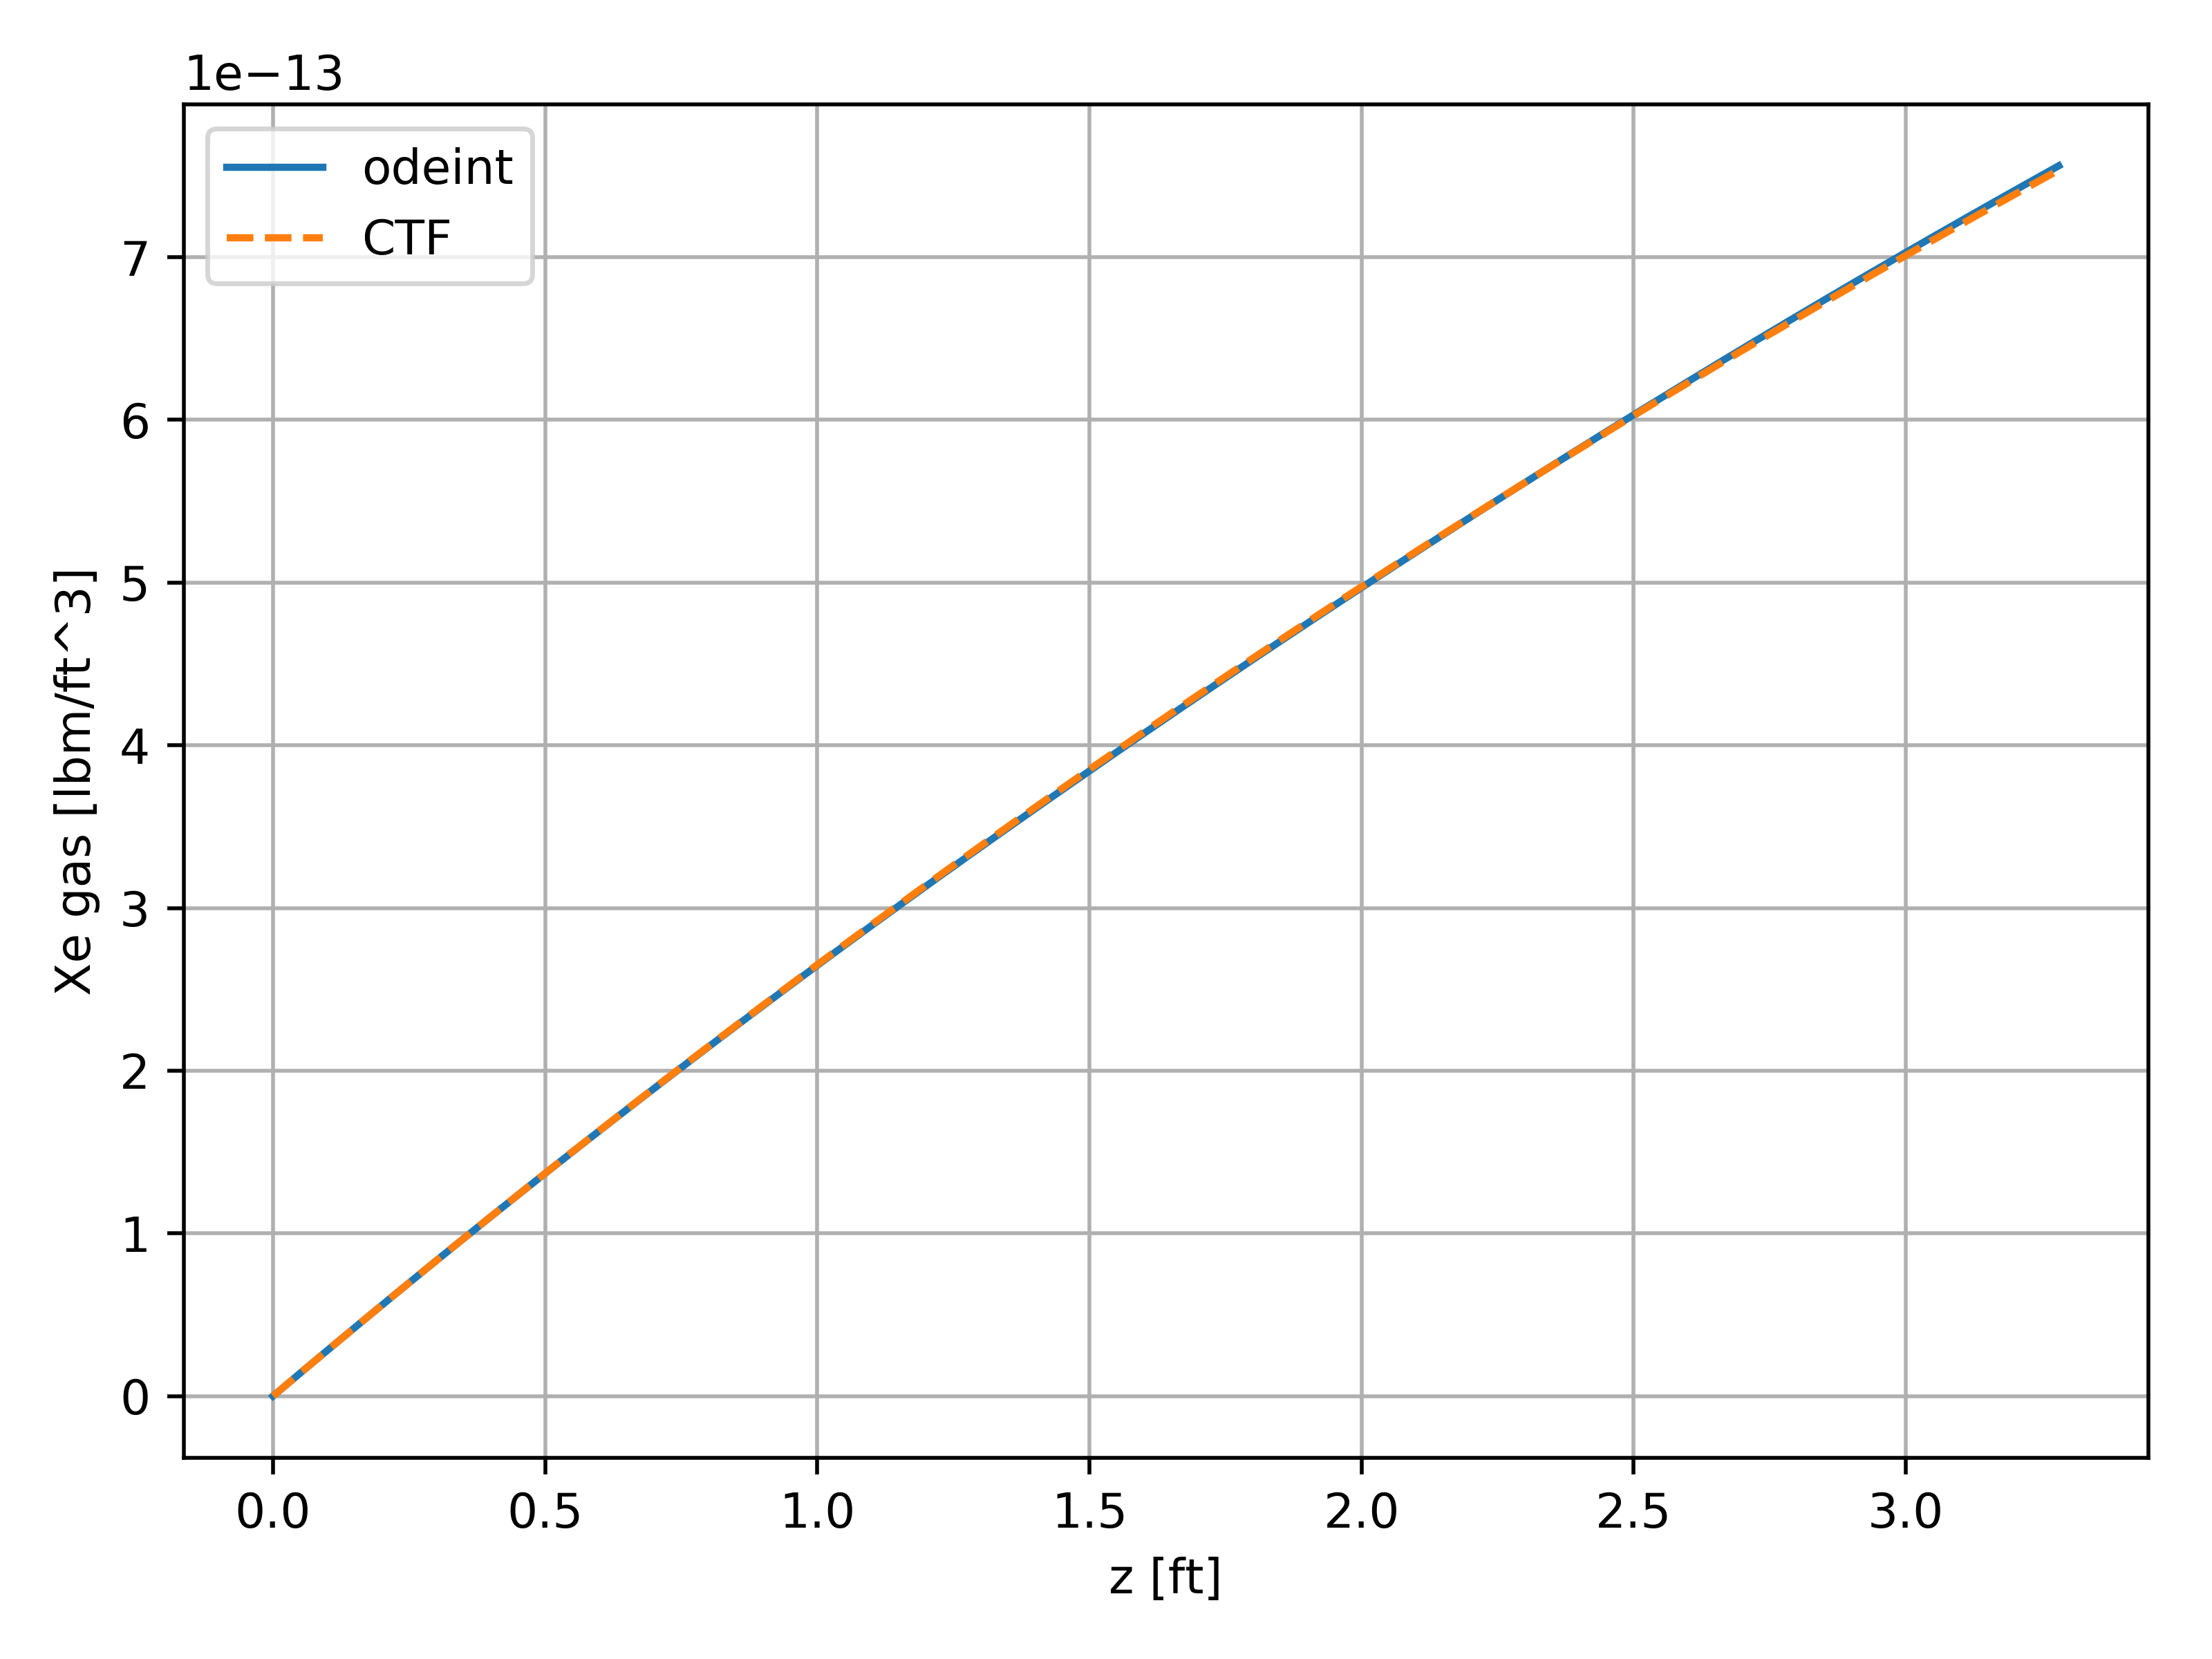
\includegraphics[width=.9\linewidth]{images/transportSpeciesIntAreaXeGas.png}
  \captionof{figure}{Xenon gas solution}
  \label{fig:IntArea_source_xe_gas_sol}
\end{minipage}%
\begin{minipage}{.5\textwidth}
  \centering
  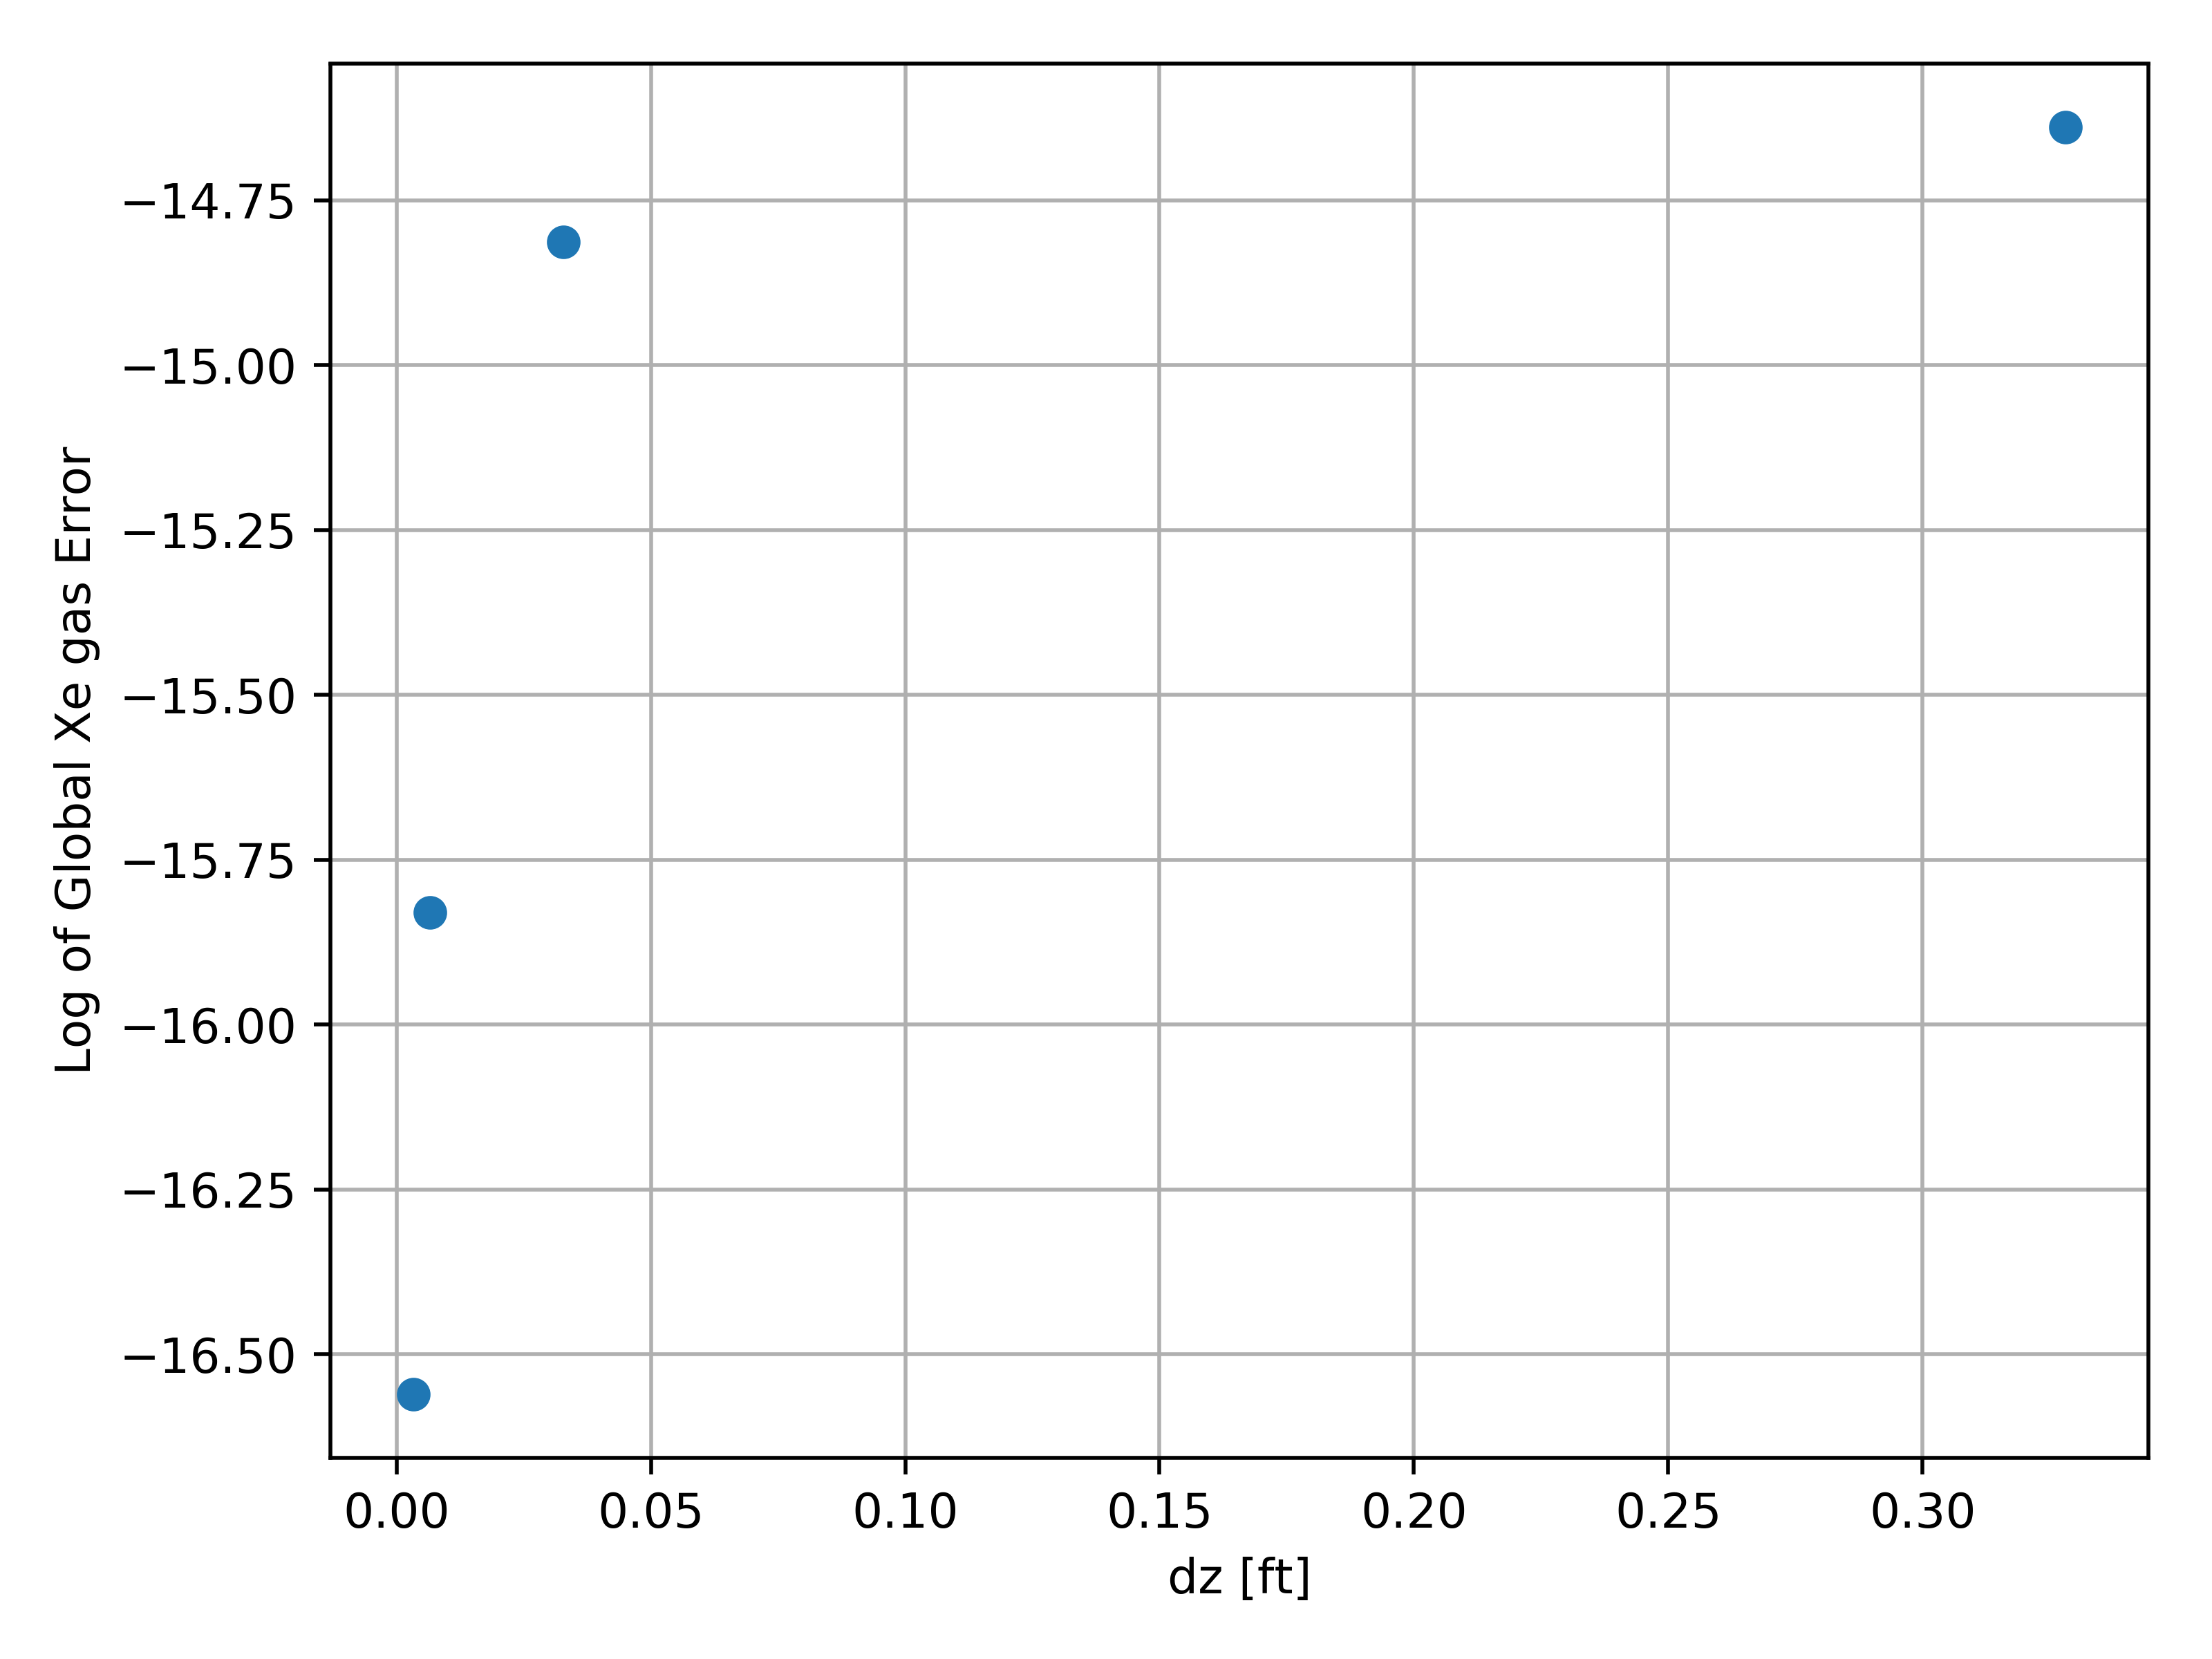
\includegraphics[width=.9\linewidth]{images/transportedSpeciesIntAreaXeGasError.png}
  \captionof{figure}{Xenon gas error vs mesh size}
  \label{fig:IntArea_source_xe_gas_error}
\end{minipage}
\end{figure}

\begin{figure}[p] 
\centering
\begin{minipage}{.5\textwidth}
  \centering
  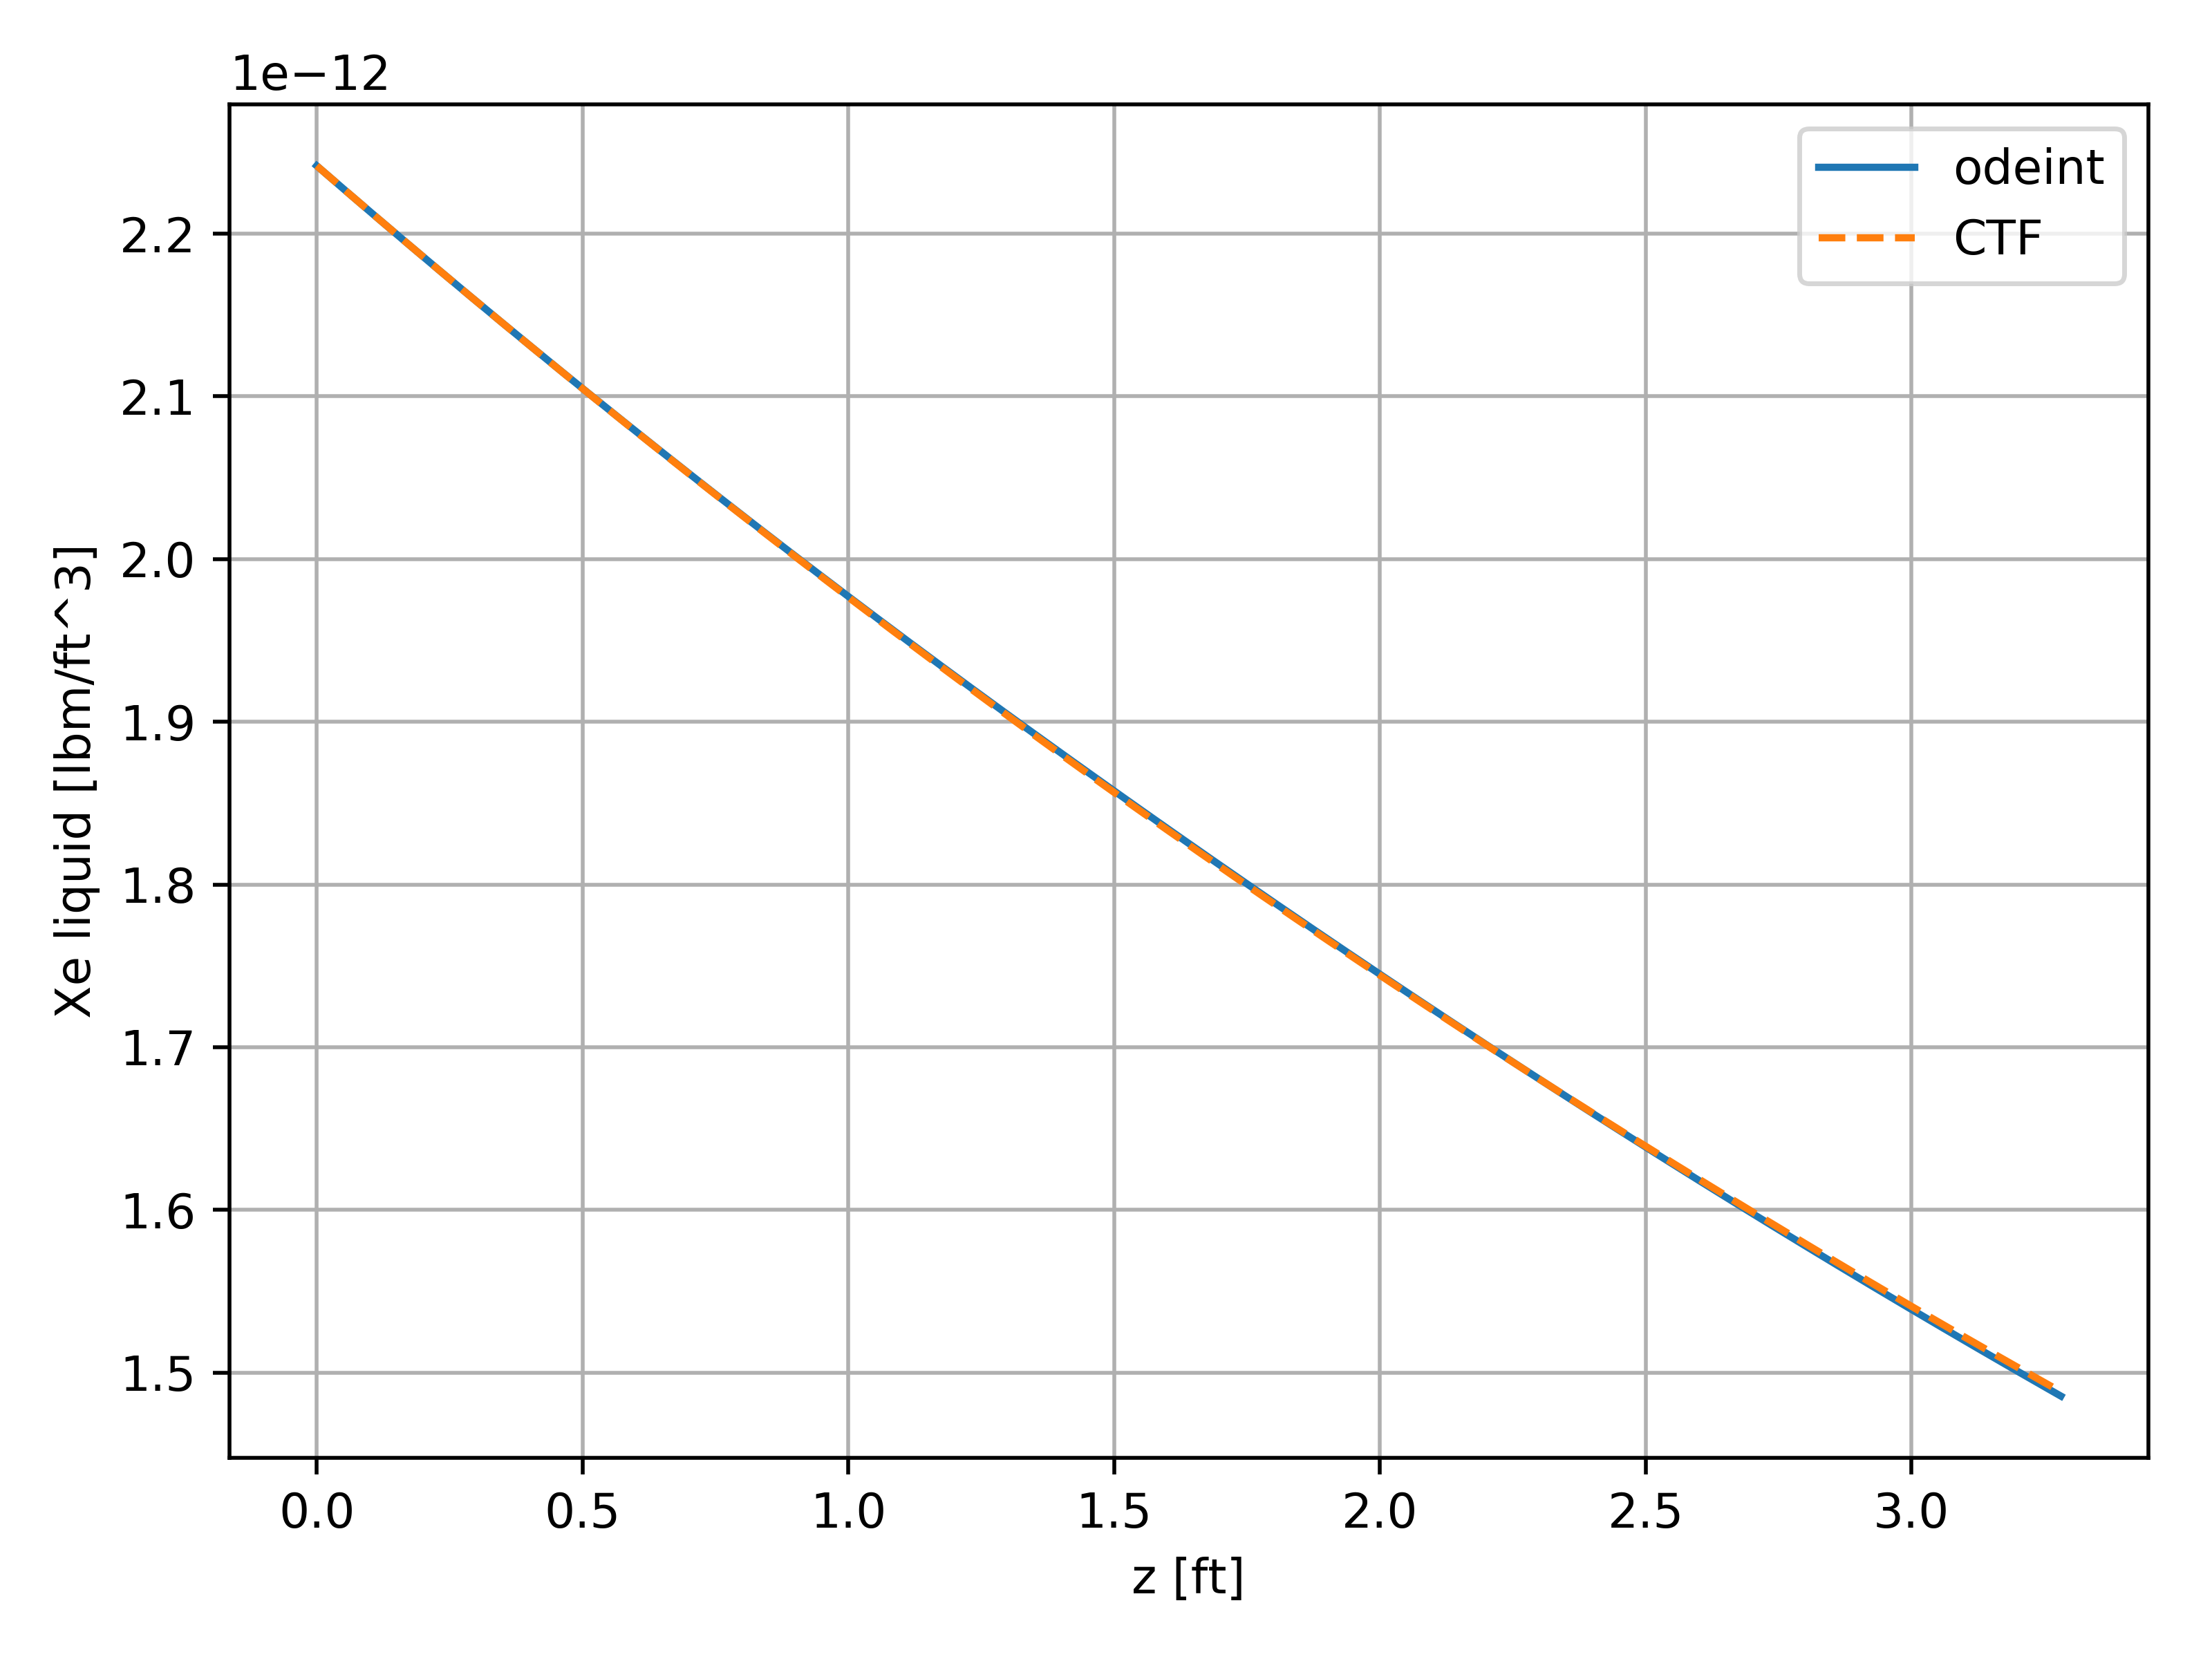
\includegraphics[width=.9\linewidth]{images/transportSpeciesIntAreaXeLiq.png}
  \captionof{figure}{Xenon liquid solution}
  \label{fig:IntArea_source_xe_liq_sol}
\end{minipage}%
\begin{minipage}{.5\textwidth}
  \centering
  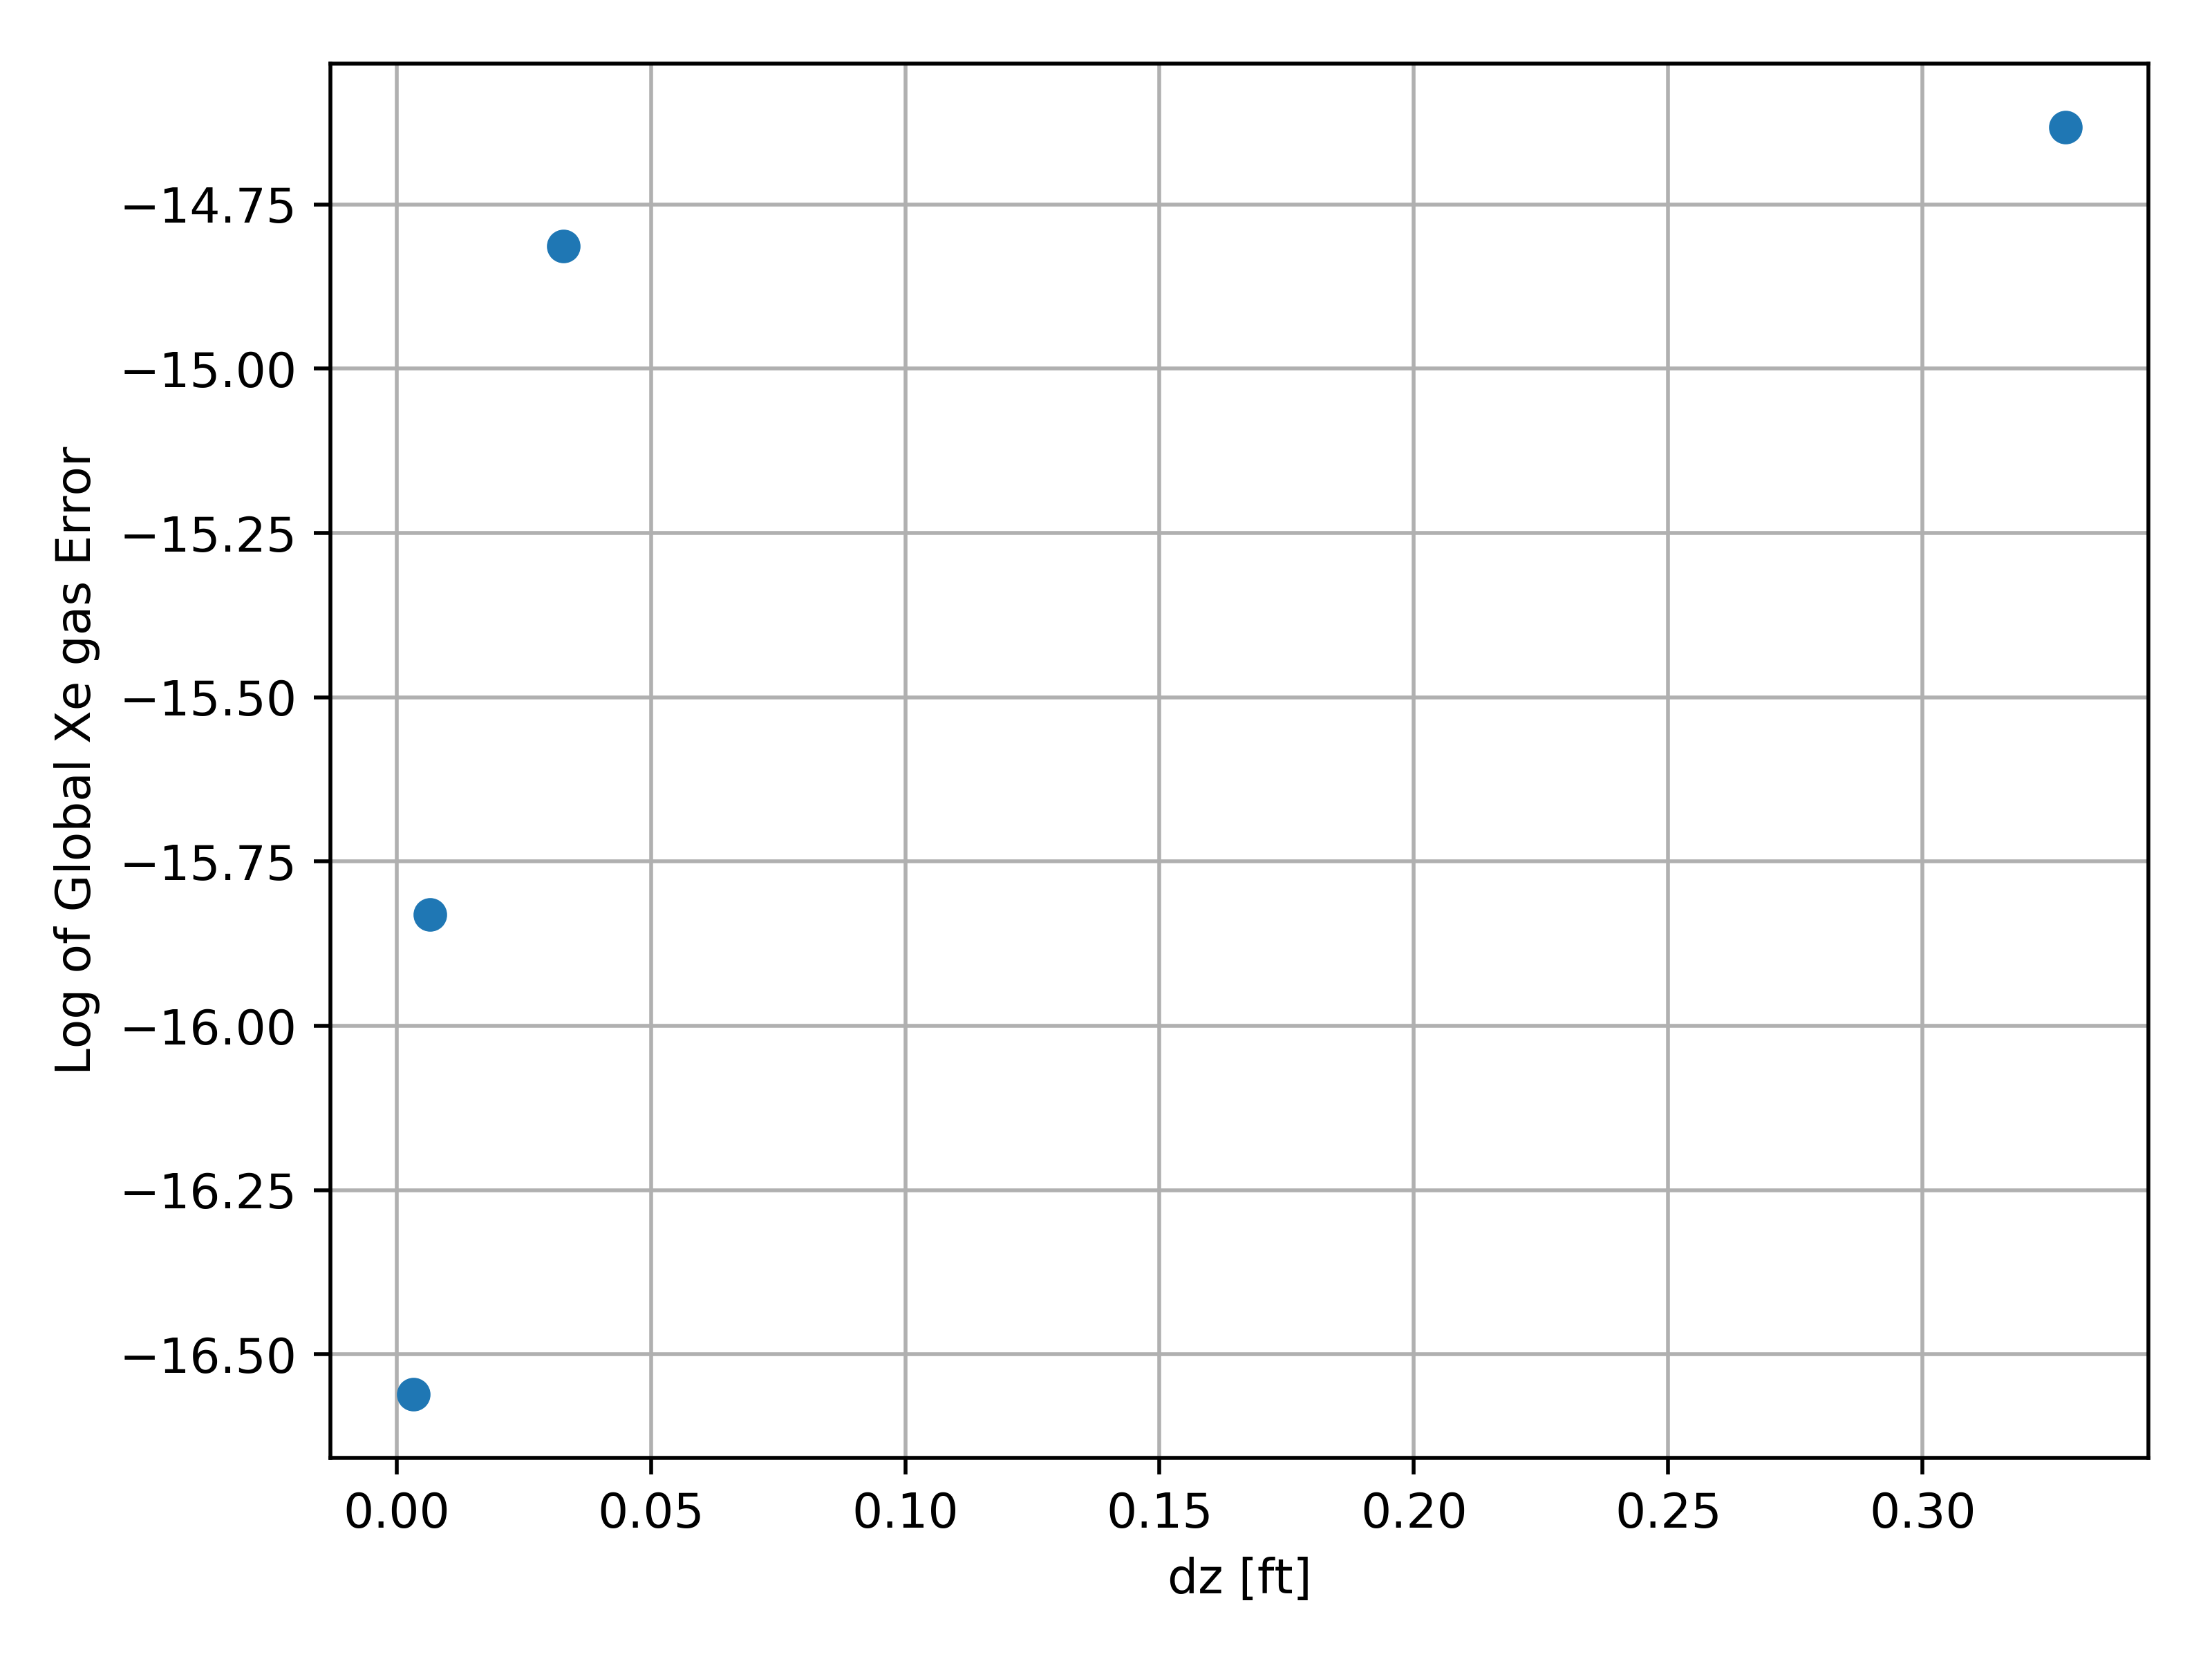
\includegraphics[width=.9\linewidth]{images/transportedSpeciesIntAreaXeLiqError.png}
  \captionof{figure}{Xenon liquid error vs mesh size}
  \label{fig:IntArea_source_xe_liq_error}
\end{minipage}
\end{figure}
\FloatBarrier
\newpage

\subsection{Bubble and Species Removal}
Gas removal was defined in \ref{ch:bubble_BC} to be a removal efficiency multiplied by the incoming flow rate of gas in the cell.  This problem consist of two channels each with 10 axial levels, shown in Figure
\ref{fig:MultiChanBubRemoval_problem}. Xenon and Helium gas bubbles are injected at the bottom of both channels in the first level. Velocity in the axial direction brings the species up and out of the channel. A velocity component is added between the channels and 1/2 the velocity in the axial direction. This causes species to migrate from channel one into channel two. In the seventh level of the second channel 80\% of the bubbles are removed from the channel, bringing with it 80\% of the species in the bubble. 

 Once the problem is run to steady state, a simple mass balance around the removal cell is used to ensure removal is properly working. From simplicity the mass flow rate coming from the bottom of the removal cell is one, from the left is two and leaving the top is three. 
 
\begin{equation}
    \dot{m_{3}} = \dot{m_{1}} + \dot{m_{2}}
    \label{eq:bubbleRemoval_mass_balance}
\end{equation}

Using the following relations between mass flow rate, flux, area and concentration, Equation \ref{eq:bubbleRemoval_mass_balance} is solved for the concentration in the removal cell.

\begin{equation}
    m_{3} = v_{z}C_{3}A_{3}; \quad m_{2} = 0.5v_{z}C_{2}A_{2}(1-S_{eff}); \quad m_{1} = v_{z}C_{1}A_{1}(1-S_{eff})
\end{equation}

Solving equation \ref{eq:bubbleRemoval_mass_balance} for the concentration in the removal cell gives:

\begin{equation}
    C_{removal} = (1-S_{eff}) \bigg[\frac{0.5C_{2}A_{2}}{A_{3}} + C_{1}\bigg]
\end{equation}

Figures \ref{fig:XeGasHeatMap}, \ref{fig:XeliqHeatMap} and \ref{fig:IntAreaConHeatMap} show the density of xenon in the gas bubbles, xenon in the liquid and interfacial area concentration respectively.  All three variables show migration from channel one to channel two due to the velocity component in the lateral direction. Both the concentrations for xenon in the gas and interfacial area drop in the removal cell. After the removal cell, interfiacal area and xenon in the gas both increase from mass transfer, and migration from channel one. 


\FloatBarrier
\newpage

\begin{figure}[ht] 
\centering
\begin{minipage}{.5\textwidth}
  \centering
  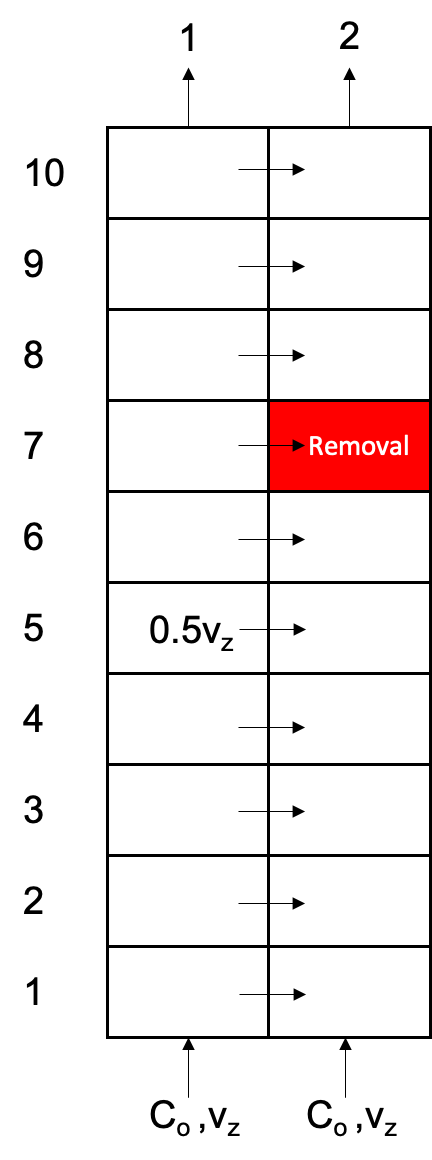
\includegraphics[width=0.78\linewidth]{images/MultiChanBubbleRemoval.png}
  \captionof{figure}{Problem domain}
  \label{fig:MultiChanBubRemoval_problem}
\end{minipage}%
\begin{minipage}{.5\textwidth}
  \centering
  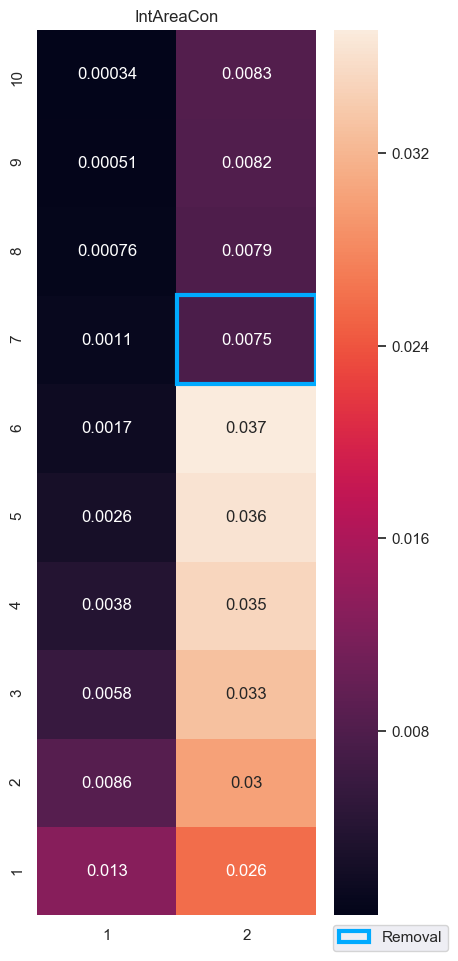
\includegraphics[width=1\linewidth]{images/IntAreaConHeatMap.png}
  \captionof{figure}{Interfacial area concentration}
  \label{fig:IntAreaConHeatMap}
\end{minipage}
\end{figure}

\begin{figure}[ht] 
\centering
\begin{minipage}{.5\textwidth}
  \centering
  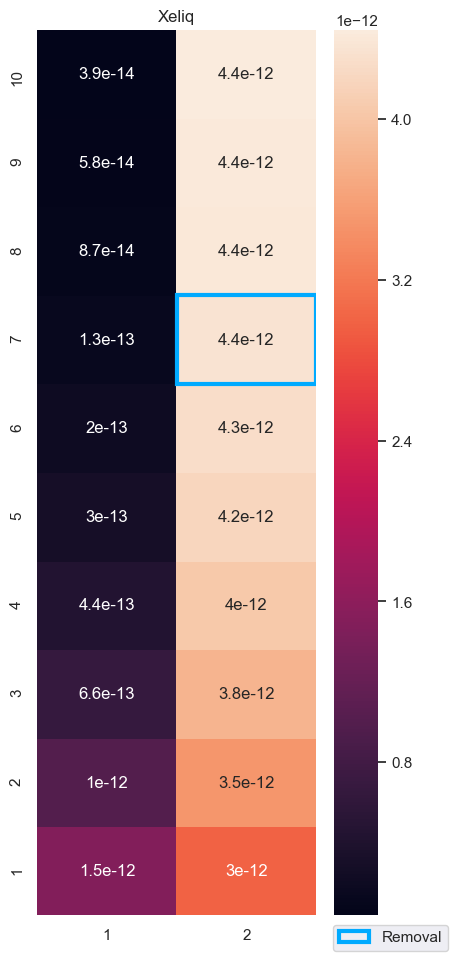
\includegraphics[width=1\linewidth]{images/XeliqHeatMap.png}
  \captionof{figure}{Xenon dissolved in the liquid}
  \label{fig:XeliqHeatMap}
\end{minipage}%
\begin{minipage}{.5\textwidth}
  \centering
  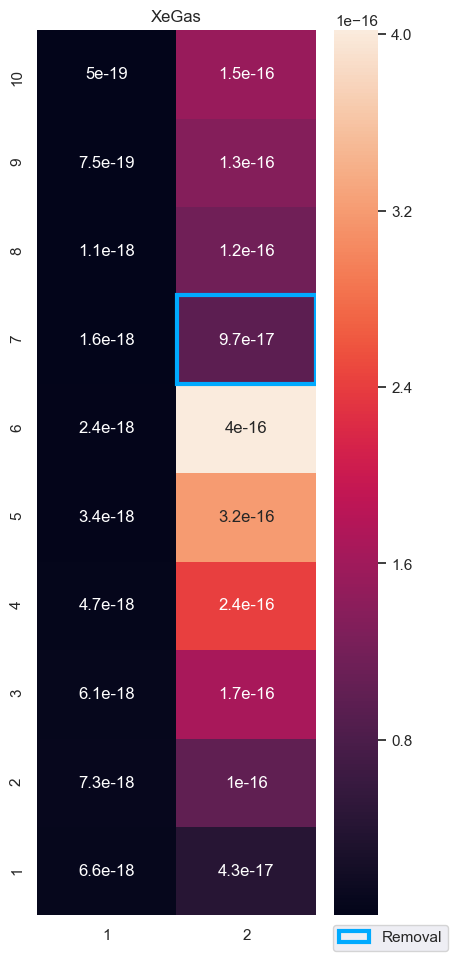
\includegraphics[width=1\linewidth]{images/XeGasHeatMap.png}
  \captionof{figure}{Xenon is the gas bubbles}
  \label{fig:XeGasHeatMap}
\end{minipage}
\end{figure}

\FloatBarrier
\newpage




\section{Case Studies}
Sections \ref{sec:gen_transport} and \ref{sec:gas_transport} demonstrated that individual components for species transport and multi-phase transport properly work. In this section we will analysis a coupled xenon iodine system, as well as how varying parameters impacts the xenon behavior. A base case is chosen from related MSRE information, then boundary conditions are changed to examine their impact on xenon in the circulating bubbles. 


The governing equations are similar to those in Equations \ref{eq:XenonGeneralDiffEq} and \ref{eq:IodineGeneralDiffEq} but with the addition of mass transfer from xenon in the liquid to xenon in the gas. These Equations are shown in \ref{eq:XenonLiqCaseStudyDiffEq} through \ref{eq:IodineLiqCaseStudyDiffEq}. A total of five species will be modeled, two for xenon, two for helium and one for iodine. One of the xenon species will denote the xenon dissolved in the molten salt and the other will denote the xenon trapped in the helium bubbles, the same goes for helium. Iodine is assumed not to migrate into the circulating void. Table \ref{tab:simple_loop_test_parameters} gives the problem parameters for the base case. The average void experienced in the MSRE was between 0.02 and 0.04 \cite{engel1971}, the Helium gas injection rate was determined using these values.

The simple loop is a scaled down version of an MSRE model, shown in Figure \ref{fig:simple_loop}. This model is broken down into six sections each with their own color code. Red is the core region, gold is the upper plenum which houses the pump. White is the heat exchanger, blue is the turn around elbow. Purple is the down comer, and black is the core inlet. 

\vspace{12.7mm} %5mm vertical space

\begin{figure}[ht]
  \centering
  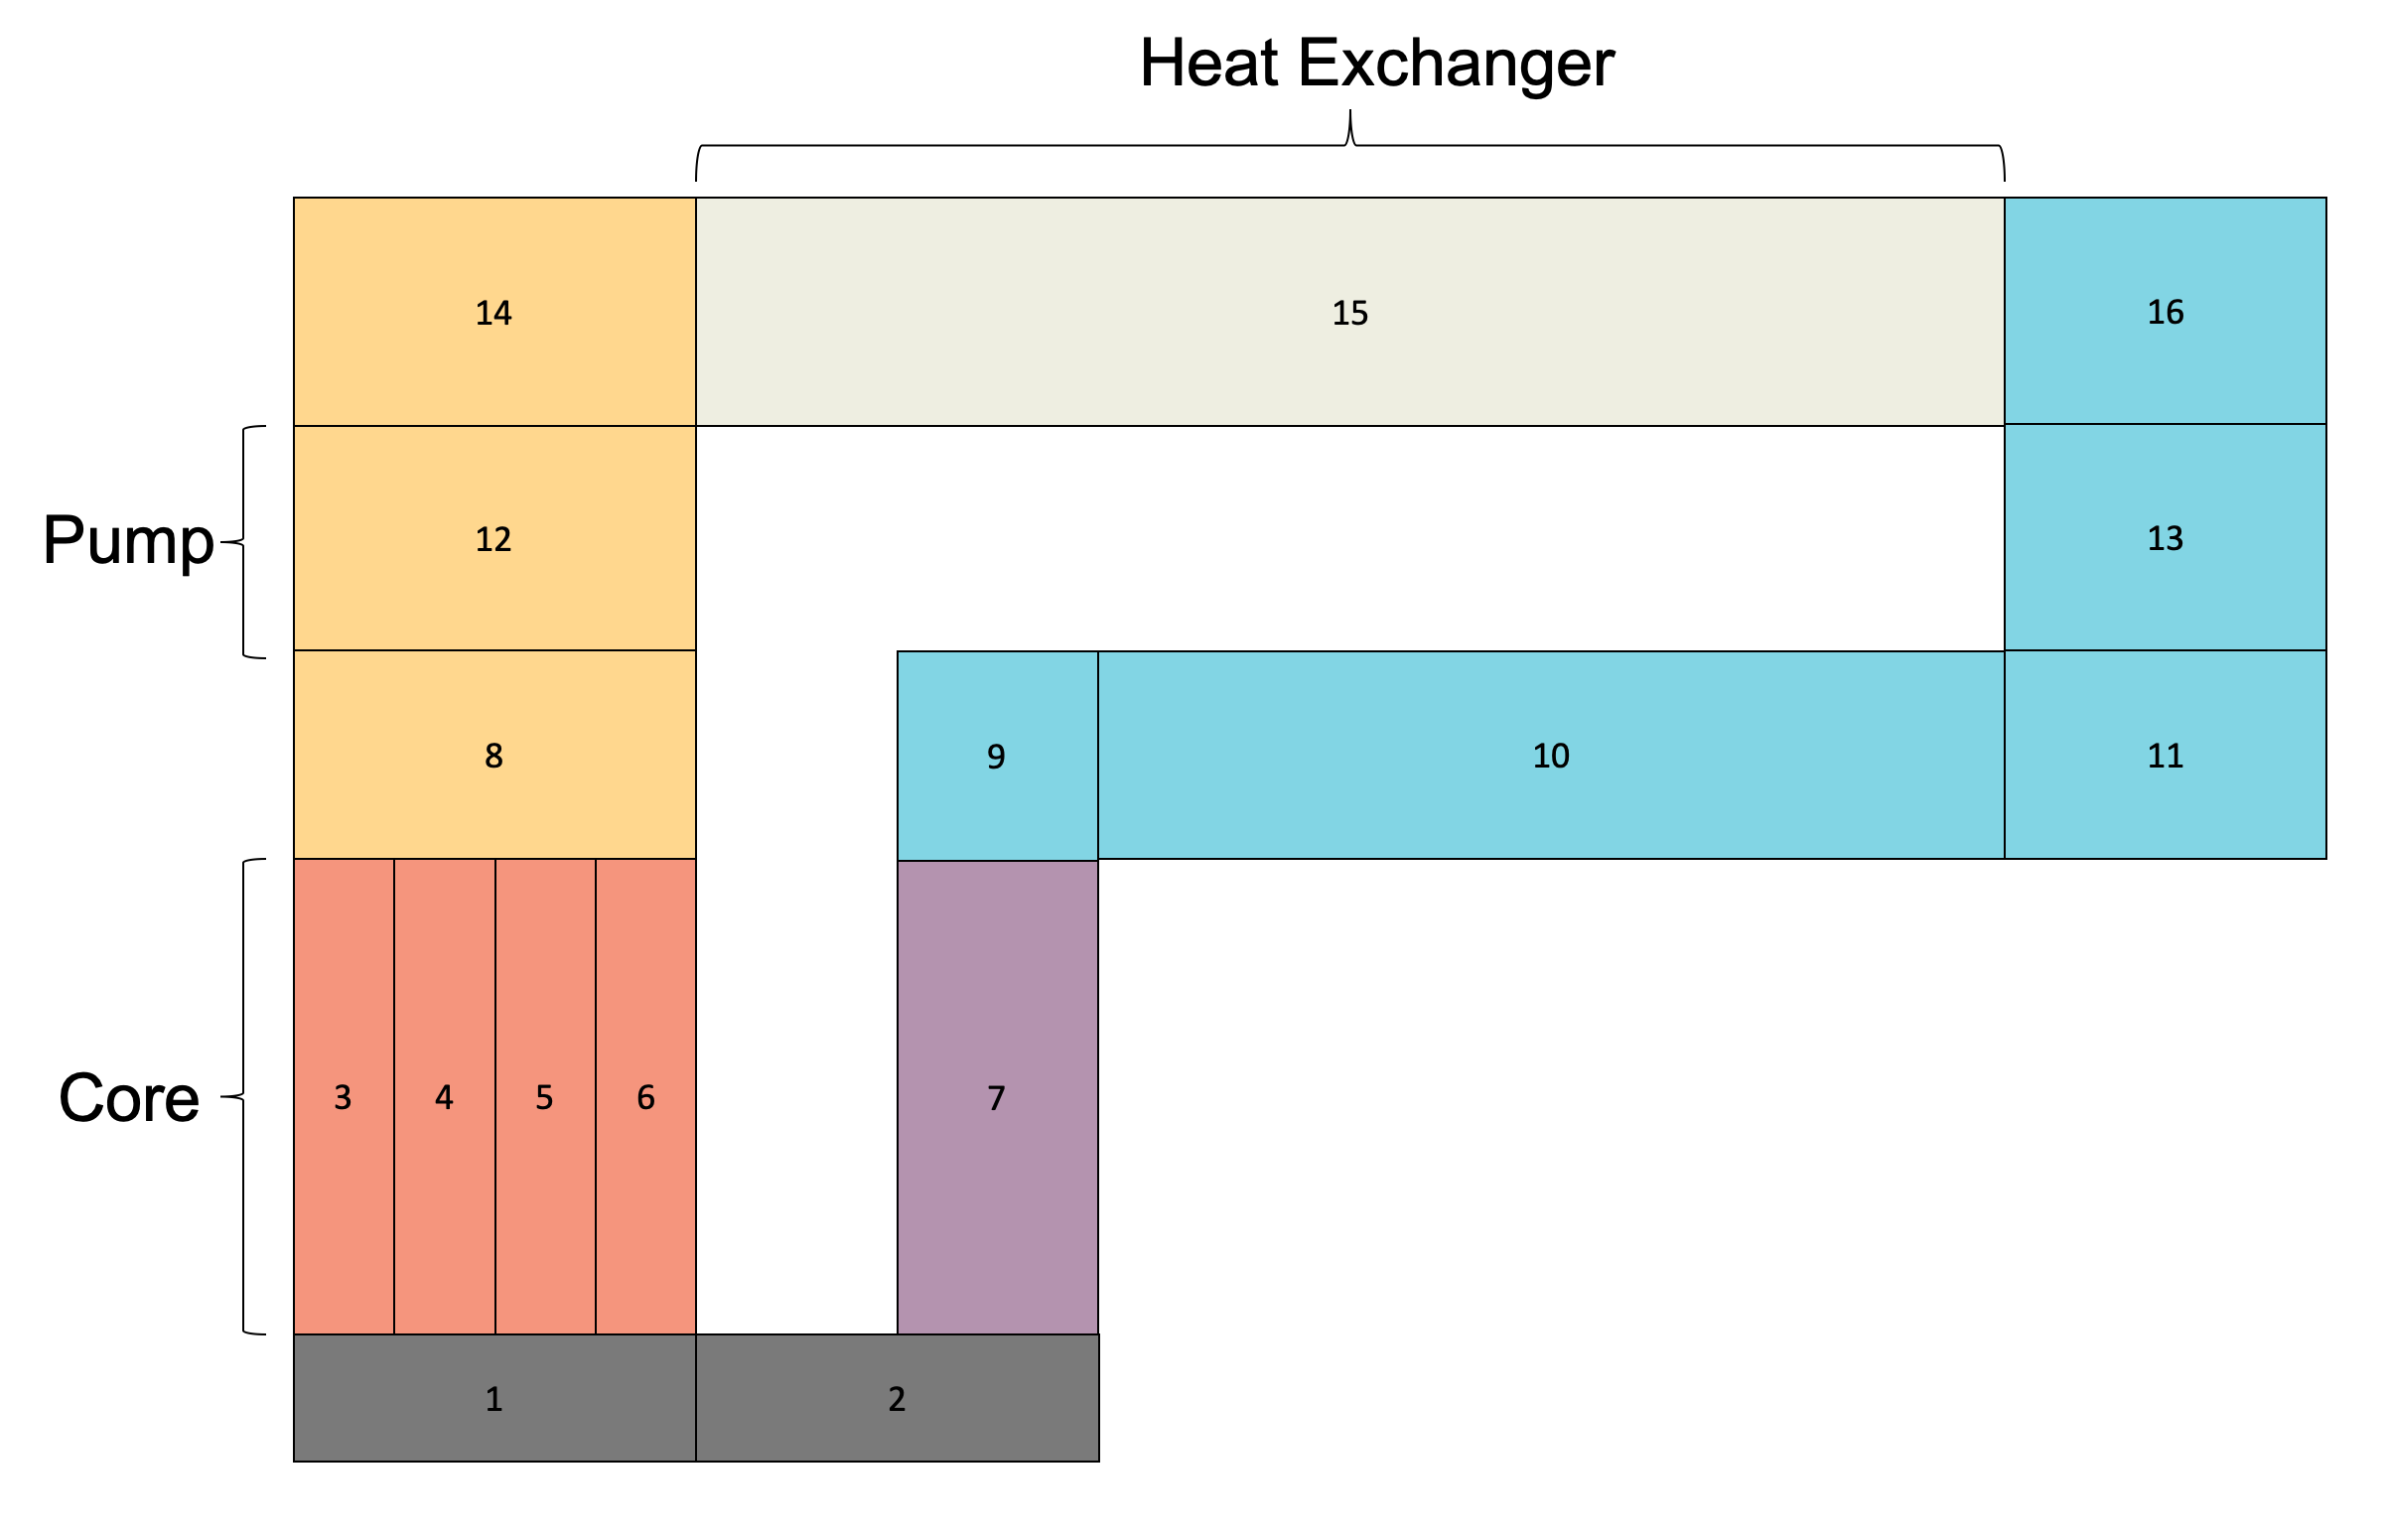
\includegraphics[width=5in]{images/simple_loop.png}\\
  \caption{Simple loop diagram}
  \label{fig:simple_loop}
\end{figure}

\begin{table}[htbp!]
   \caption{\label{tab:simple_loop_test_parameters} Base case parameters}
   \centering
   \begin{tabular}{lll}
   \hline
   \textbf{Parameter} & \textbf{Value} & \textbf{Unit} \\
   \hline 
   $\gamma_{I}$ & $6.3033$ \cite{cole2019}& $\%$ \\ [1ex]
   $\gamma_{Xe}$ & 0.2468 \cite{cole2019}& \% \\ [1ex]
   $\Sigma_{f}$ & 9.7532E-1 \cite{cole2019}& 1/ft \\ [1ex]
   $\Phi$ & $2.5E16$ \cite{nestor1960}& $n/ft^{2}/s$ \\ [1ex]
   $\lambda_{Xe}$ & 2.11E-5 \cite{cole2019}& 1/s\\ [1ex]
   $\lambda_{I}$ & 2.9306E-5 \cite{cole2019}& 1/s  \\ [1ex]
   $M_{Xe}$ & 135.0 & lbm/mol\\ [1ex]
   $M_{I}$ & 135.0 & lbm/mol \\ [1ex]
   $M_{He}$ & 4.0 & lbm/mol \\ [1ex]
   $k_{Xe}$ & 2.0 \cite{houtzeel1967} & ft/hr\\ [1ex]
   $k_{He}$ & 4.0 \cite{engel1971} & ft/hr \\ [1ex]
   $H_{Xe}$ & 2.75E-9 \cite{houtzeel1967} & mole/cm${}^{3}$/atm \\ [1ex]
   $H_{He}$ & 1.26E-7 \cite{engel1971} & mole/cm${}^{3}$/atm \\ [1ex]
   $D_{ref}$ & 0.03175${}^{a}$  & cm \\ [1ex]
   He injection rate & 2.0E-5 & moles/s \\ [1ex]
   Removal efficiency & 0.99 & \% \\ [1ex] 
   $\alpha$ Void fraction & - & - \\ [1ex]
   \hline
      \end{tabular}
    \begin{tablenotes}\footnotesize
   \item[a] This value is the average for the range of bubbles considered in the MSRE 0.0127-0.0508 cm \cite{engel1971}
   \end{tablenotes}

\end{table}

% xenon liq
\begin{equation}
\begin{split}
    \frac{\partial \rho_{Xe}^{l}}{\partial t} = -\nabla (\rho_{Xe}^{l}v) + \frac{M_{Xe}}{N_{A}(1-\alpha)} \gamma_{Xe}\Sigma_{f}\Phi + \frac{M_{Xe}}{M_{I}}\lambda_{I}\rho_{I} -  \\ \lambda_{Xe}\rho_{Xe} - \sigma_{a}\Phi\rho_{Xe} +   \frac{Ka}{V}\Big[\rho_{Xe}^{*} - \frac{\rho_{Xe}^{l}}{1-\alpha}\Big]
    \label{eq:XenonLiqCaseStudyDiffEq}
\end{split}
\end{equation}

% xenon gas
\begin{equation}
    \frac{\partial \rho_{Xe}^{g}}{\partial t} = -\nabla (\rho_{Xe}^{g}v) + \frac{Ka}{V}\Big[\frac{\rho_{Xe}^{l}}{1-\alpha}  - \rho_{Xe}^{*}\Big]
    \label{eq:XenonGasCaseStudyDiffEq}
\end{equation}

% helium gas
\begin{equation}
    \frac{\partial \rho_{He}^{g}}{\partial t} = -\nabla (\rho_{He}^{g}v) + \frac{Ka}{V}\Big[\frac{\rho_{He}^{l}}{1-\alpha}  - \rho_{He}^{*}\Big]
    \label{eq:HeGasCaseStudyDiffEq}
\end{equation}

% helium liquid
\begin{equation}
    \frac{\partial \rho_{He}^{l}}{\partial t} = -\nabla (\rho_{He}^{l}v) + \frac{Ka}{V}\Big[ \rho_{He}^{*} - \frac{\rho_{He}^{l}}{1-\alpha}\Big]
    \label{eq:heliumLiqCaseStudyDiffEq}
\end{equation}

% iodine liquid
\begin{equation}
    \frac{\partial \rho_{I}^{l}}{\partial t} = -\nabla (\rho_{I}^{l}v) + \frac{M_{I}}{N_{A}(1-\alpha)} \gamma_{I}\Sigma_{f}\Phi - \lambda_{I}\rho_{I}
    \label{eq:IodineLiqCaseStudyDiffEq}
\end{equation}

\subsection{Base Case Results}
All cases hear forth are ran using the explicit method for a run time of 1000 seconds (dt=1.0E-2) to allow the system to reach steady state. quantities of xenon dissolved in the liquid and trapped in the gas bubbles will be in atoms per foot cubed. In nuclear engineering it is common to use atomic densities. Helium both in the bubbles and dissolved in the liquid will be in moles per foot cubed. Along with the for mentioned variables, interfacial area, bubble diameter, void and percent xenon in the bubbles are also analysed. These variables will be used at the metrics for comparing the relative cases. Shown in Figure \ref{fig:BaseCaseTemp} to \ref{fig:BaseCaseXePercent} are the base case results.

\vspace{12.7mm} %5mm vertical space

% Temp and Press
\begin{figure}[ht] 
\centering
\begin{minipage}{.5\textwidth}
  \centering
  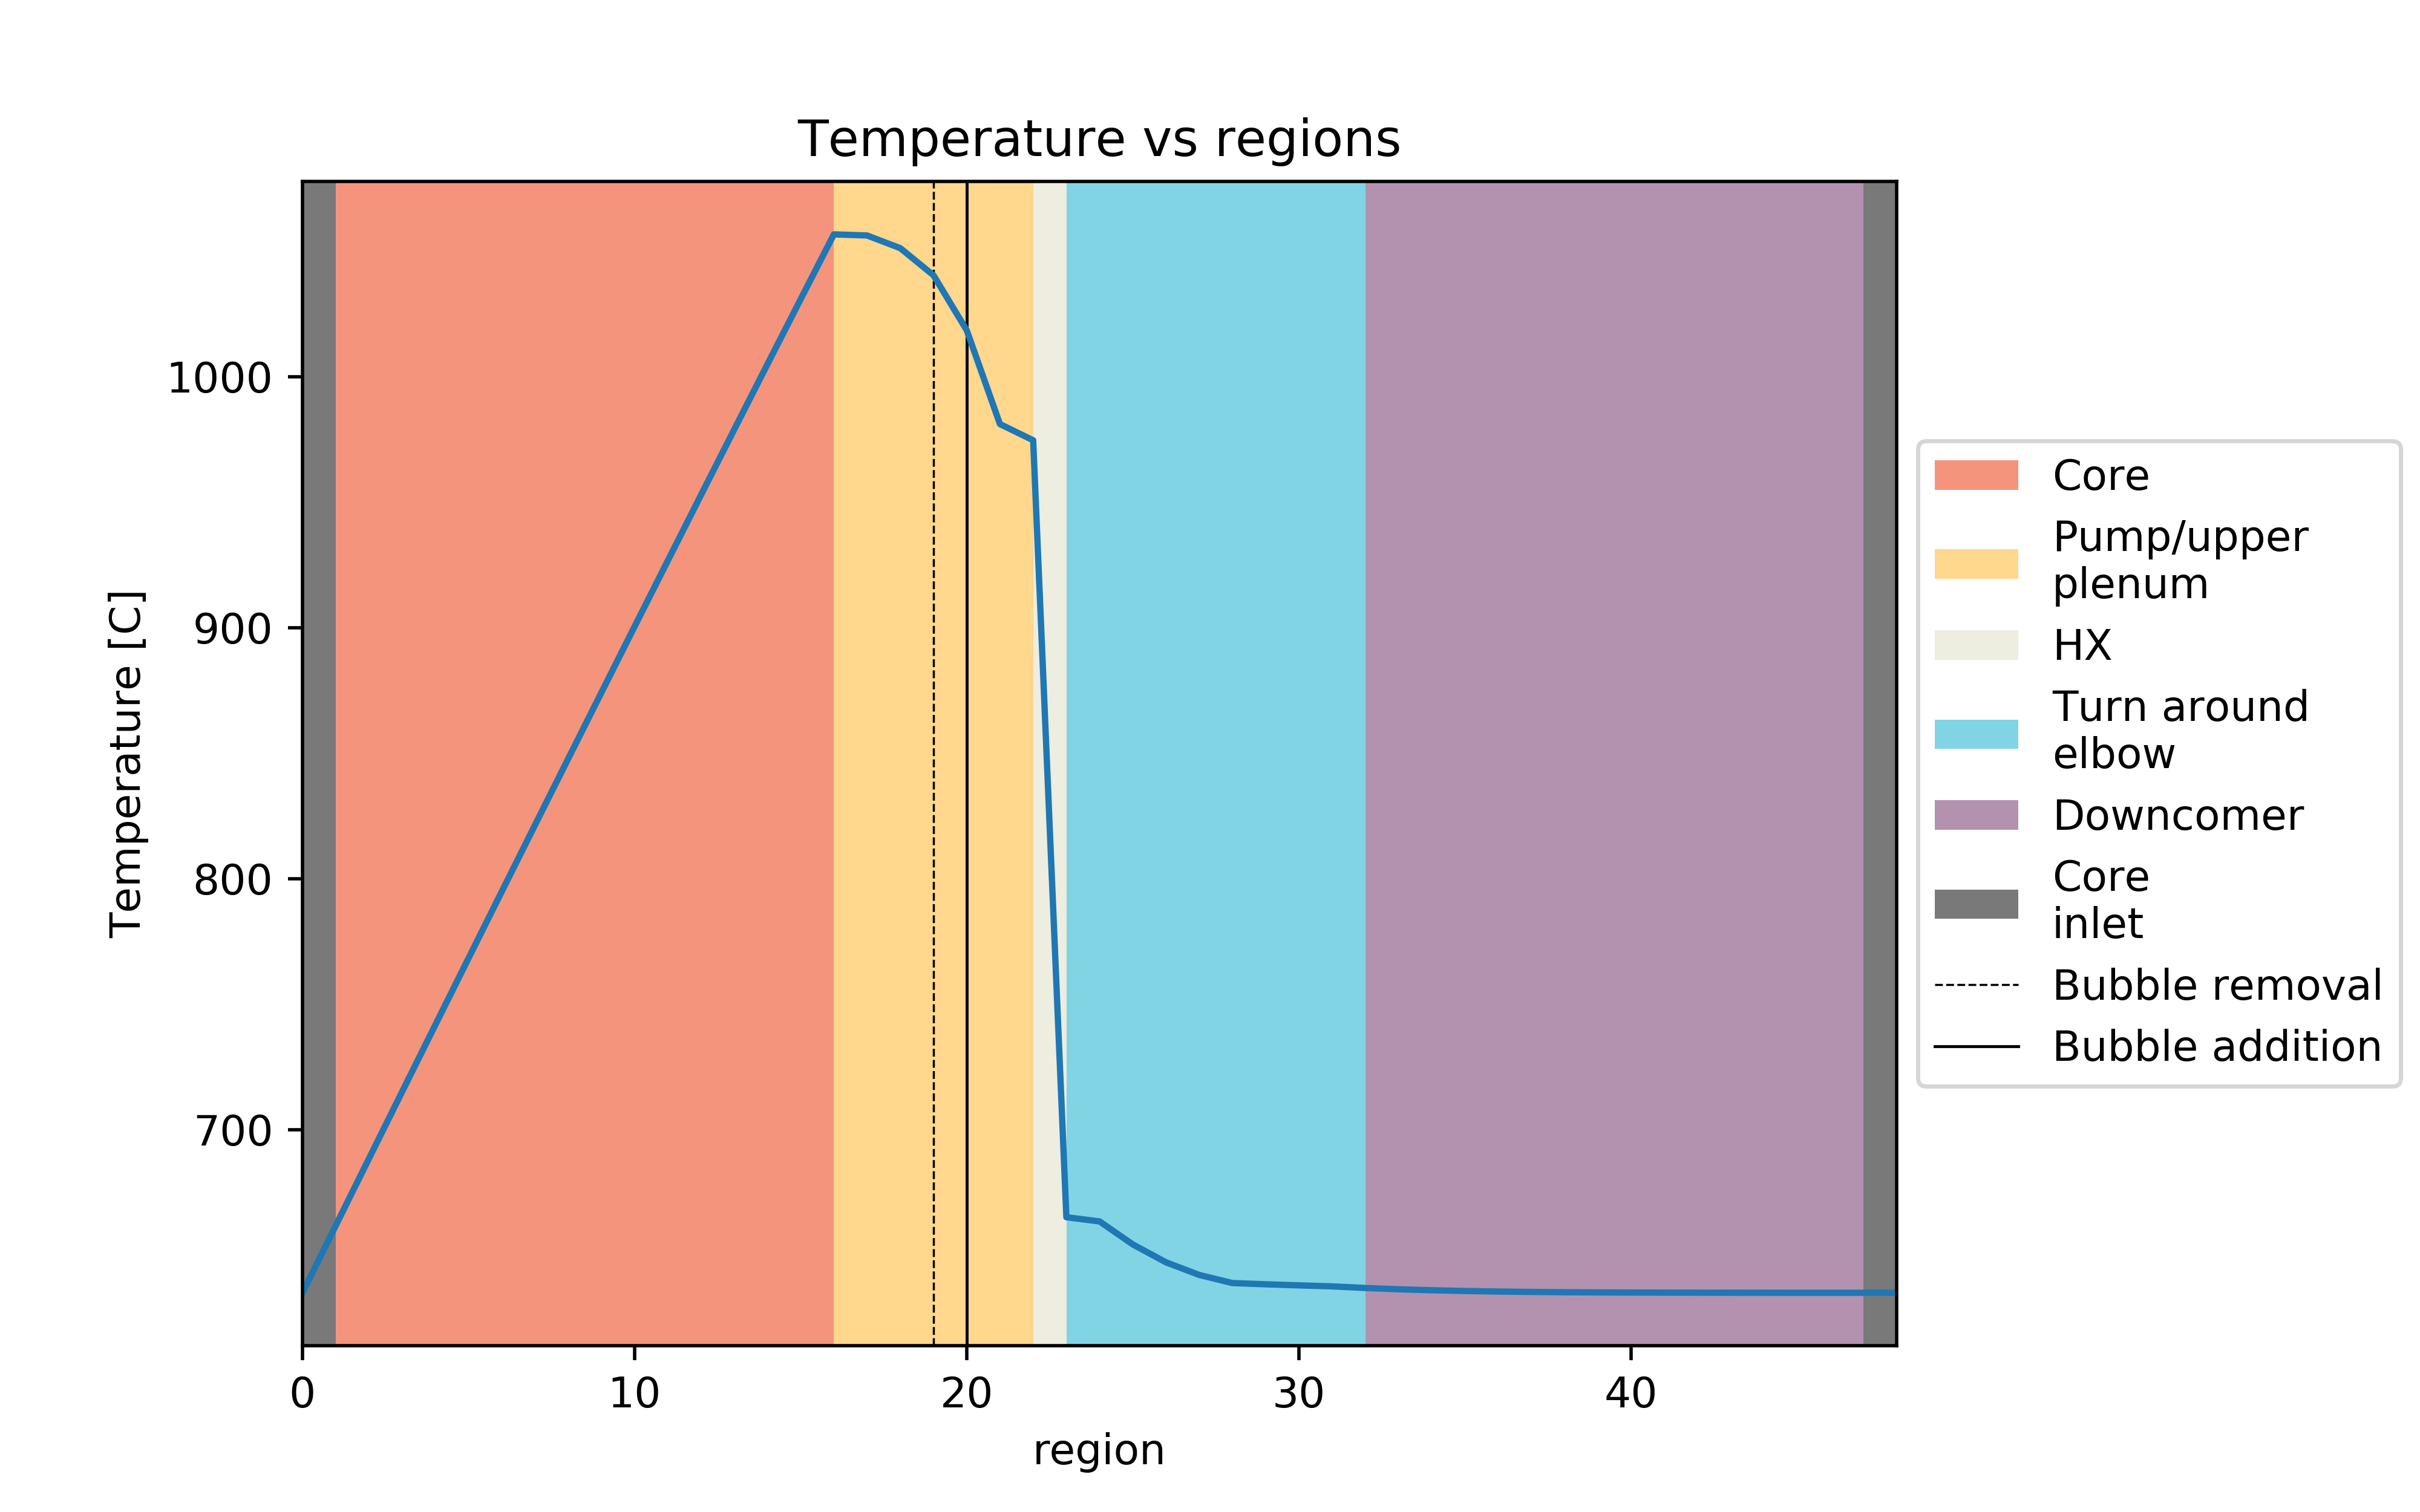
\includegraphics[width=1.0\linewidth]{images/BaseCaseTemperature.png}
  \captionof{figure}{Temperature}
  \label{fig:BaseCaseTemp}
\end{minipage}%
\begin{minipage}{.5\textwidth}
  \centering
  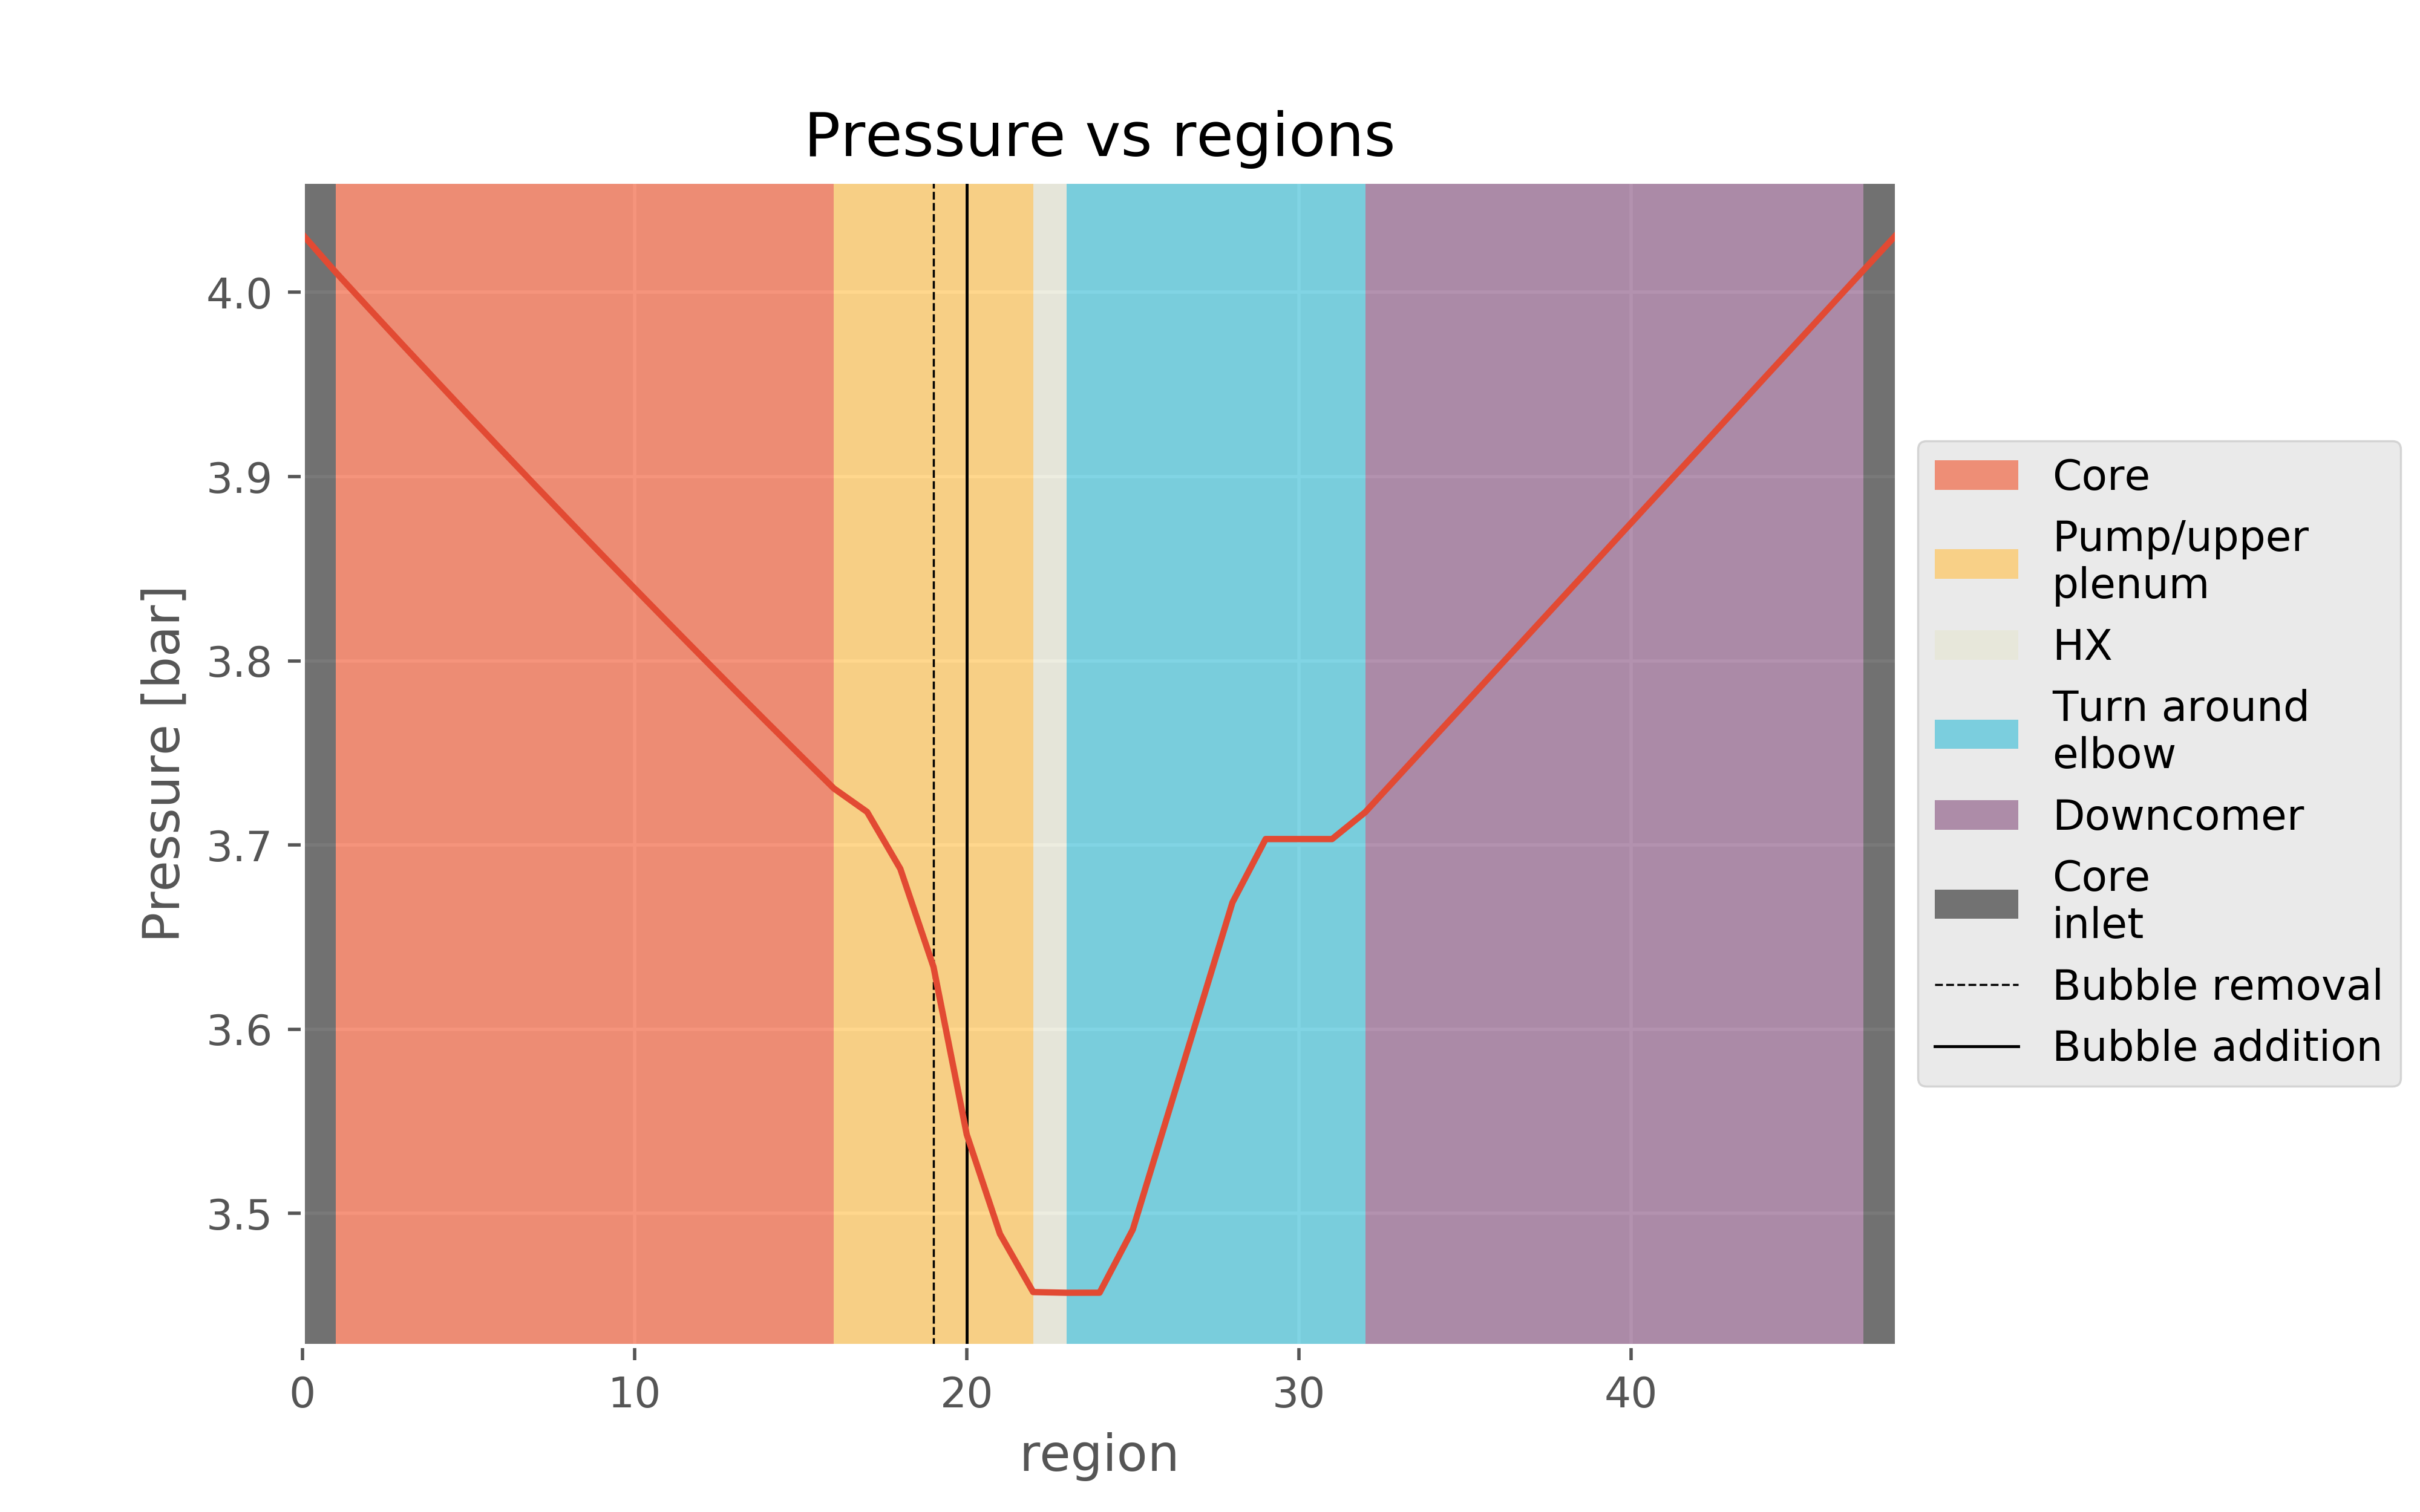
\includegraphics[width=1.0\linewidth]{images/BaseCasePressure.png}
  \captionof{figure}{Pressure}
  \label{fig:BaseCasePress}
\end{minipage}
\end{figure}

% void and diameter
\begin{figure}[ht] 
\centering
\begin{minipage}{.5\textwidth}
  \centering
  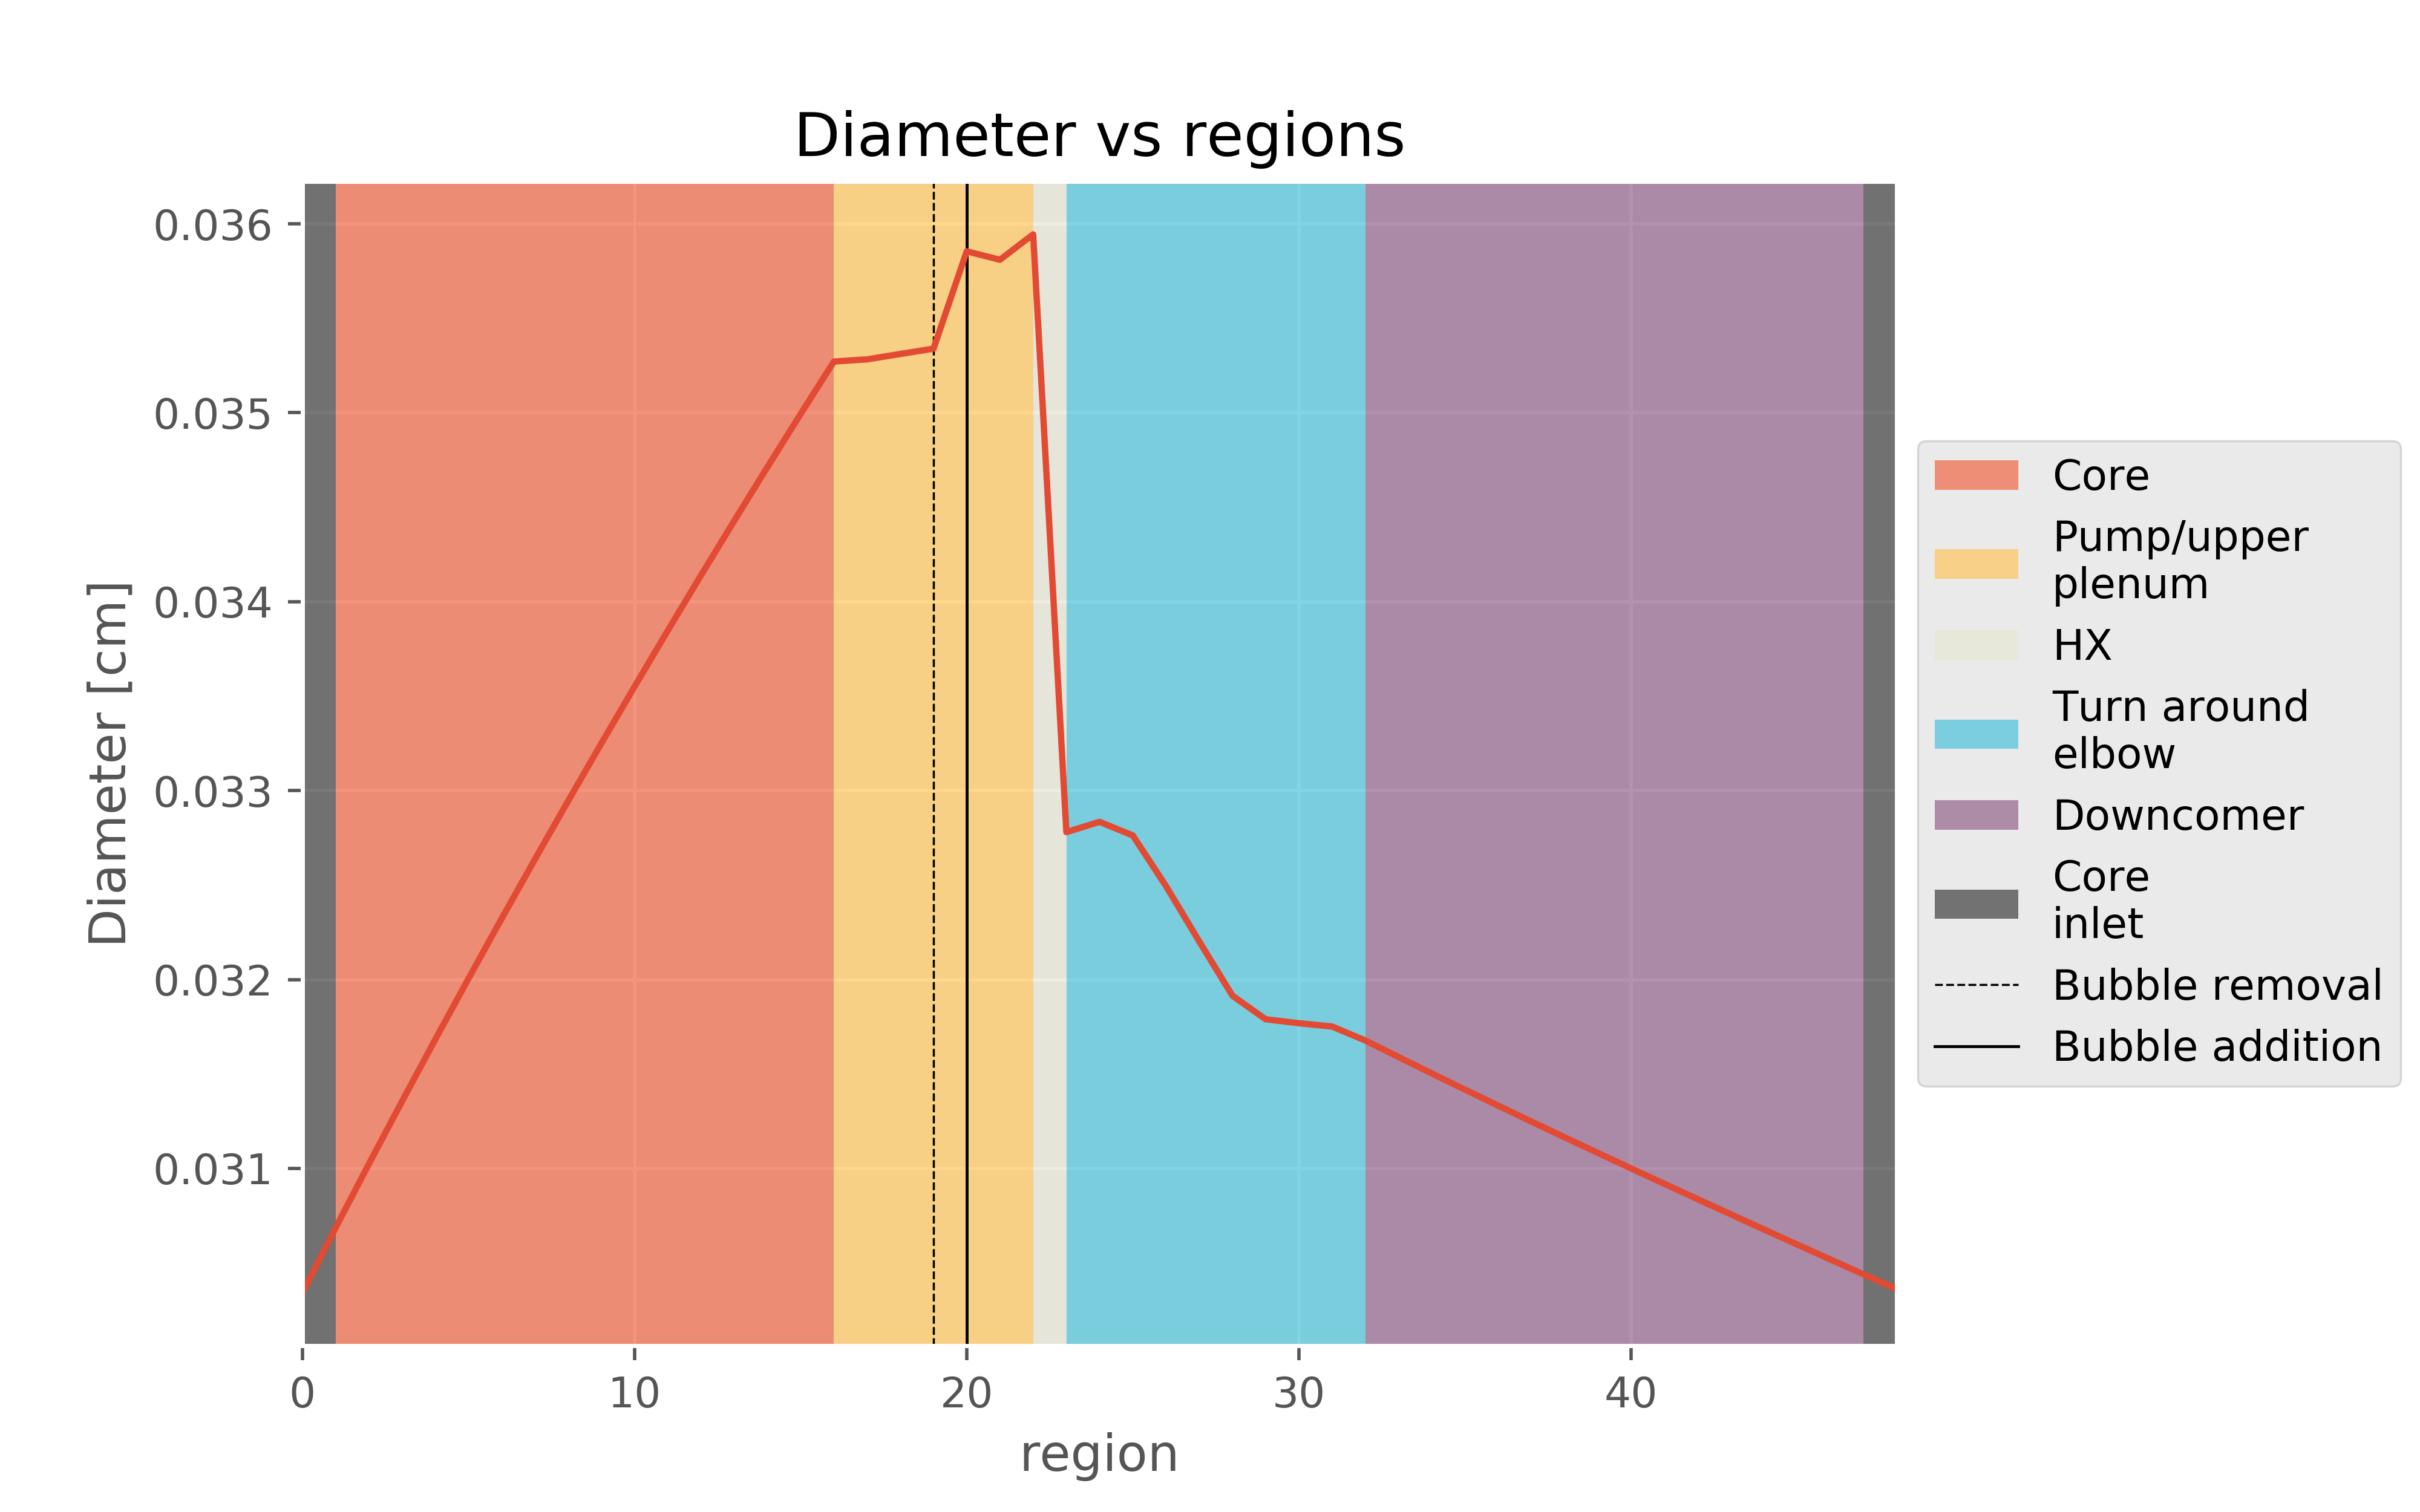
\includegraphics[width=1.0\linewidth]{images/BaseCaseDiameter.png}
  \captionof{figure}{Bubble diameter}
  \label{fig:BaseCaseDia}
\end{minipage}%
\begin{minipage}{.5\textwidth}
  \centering
  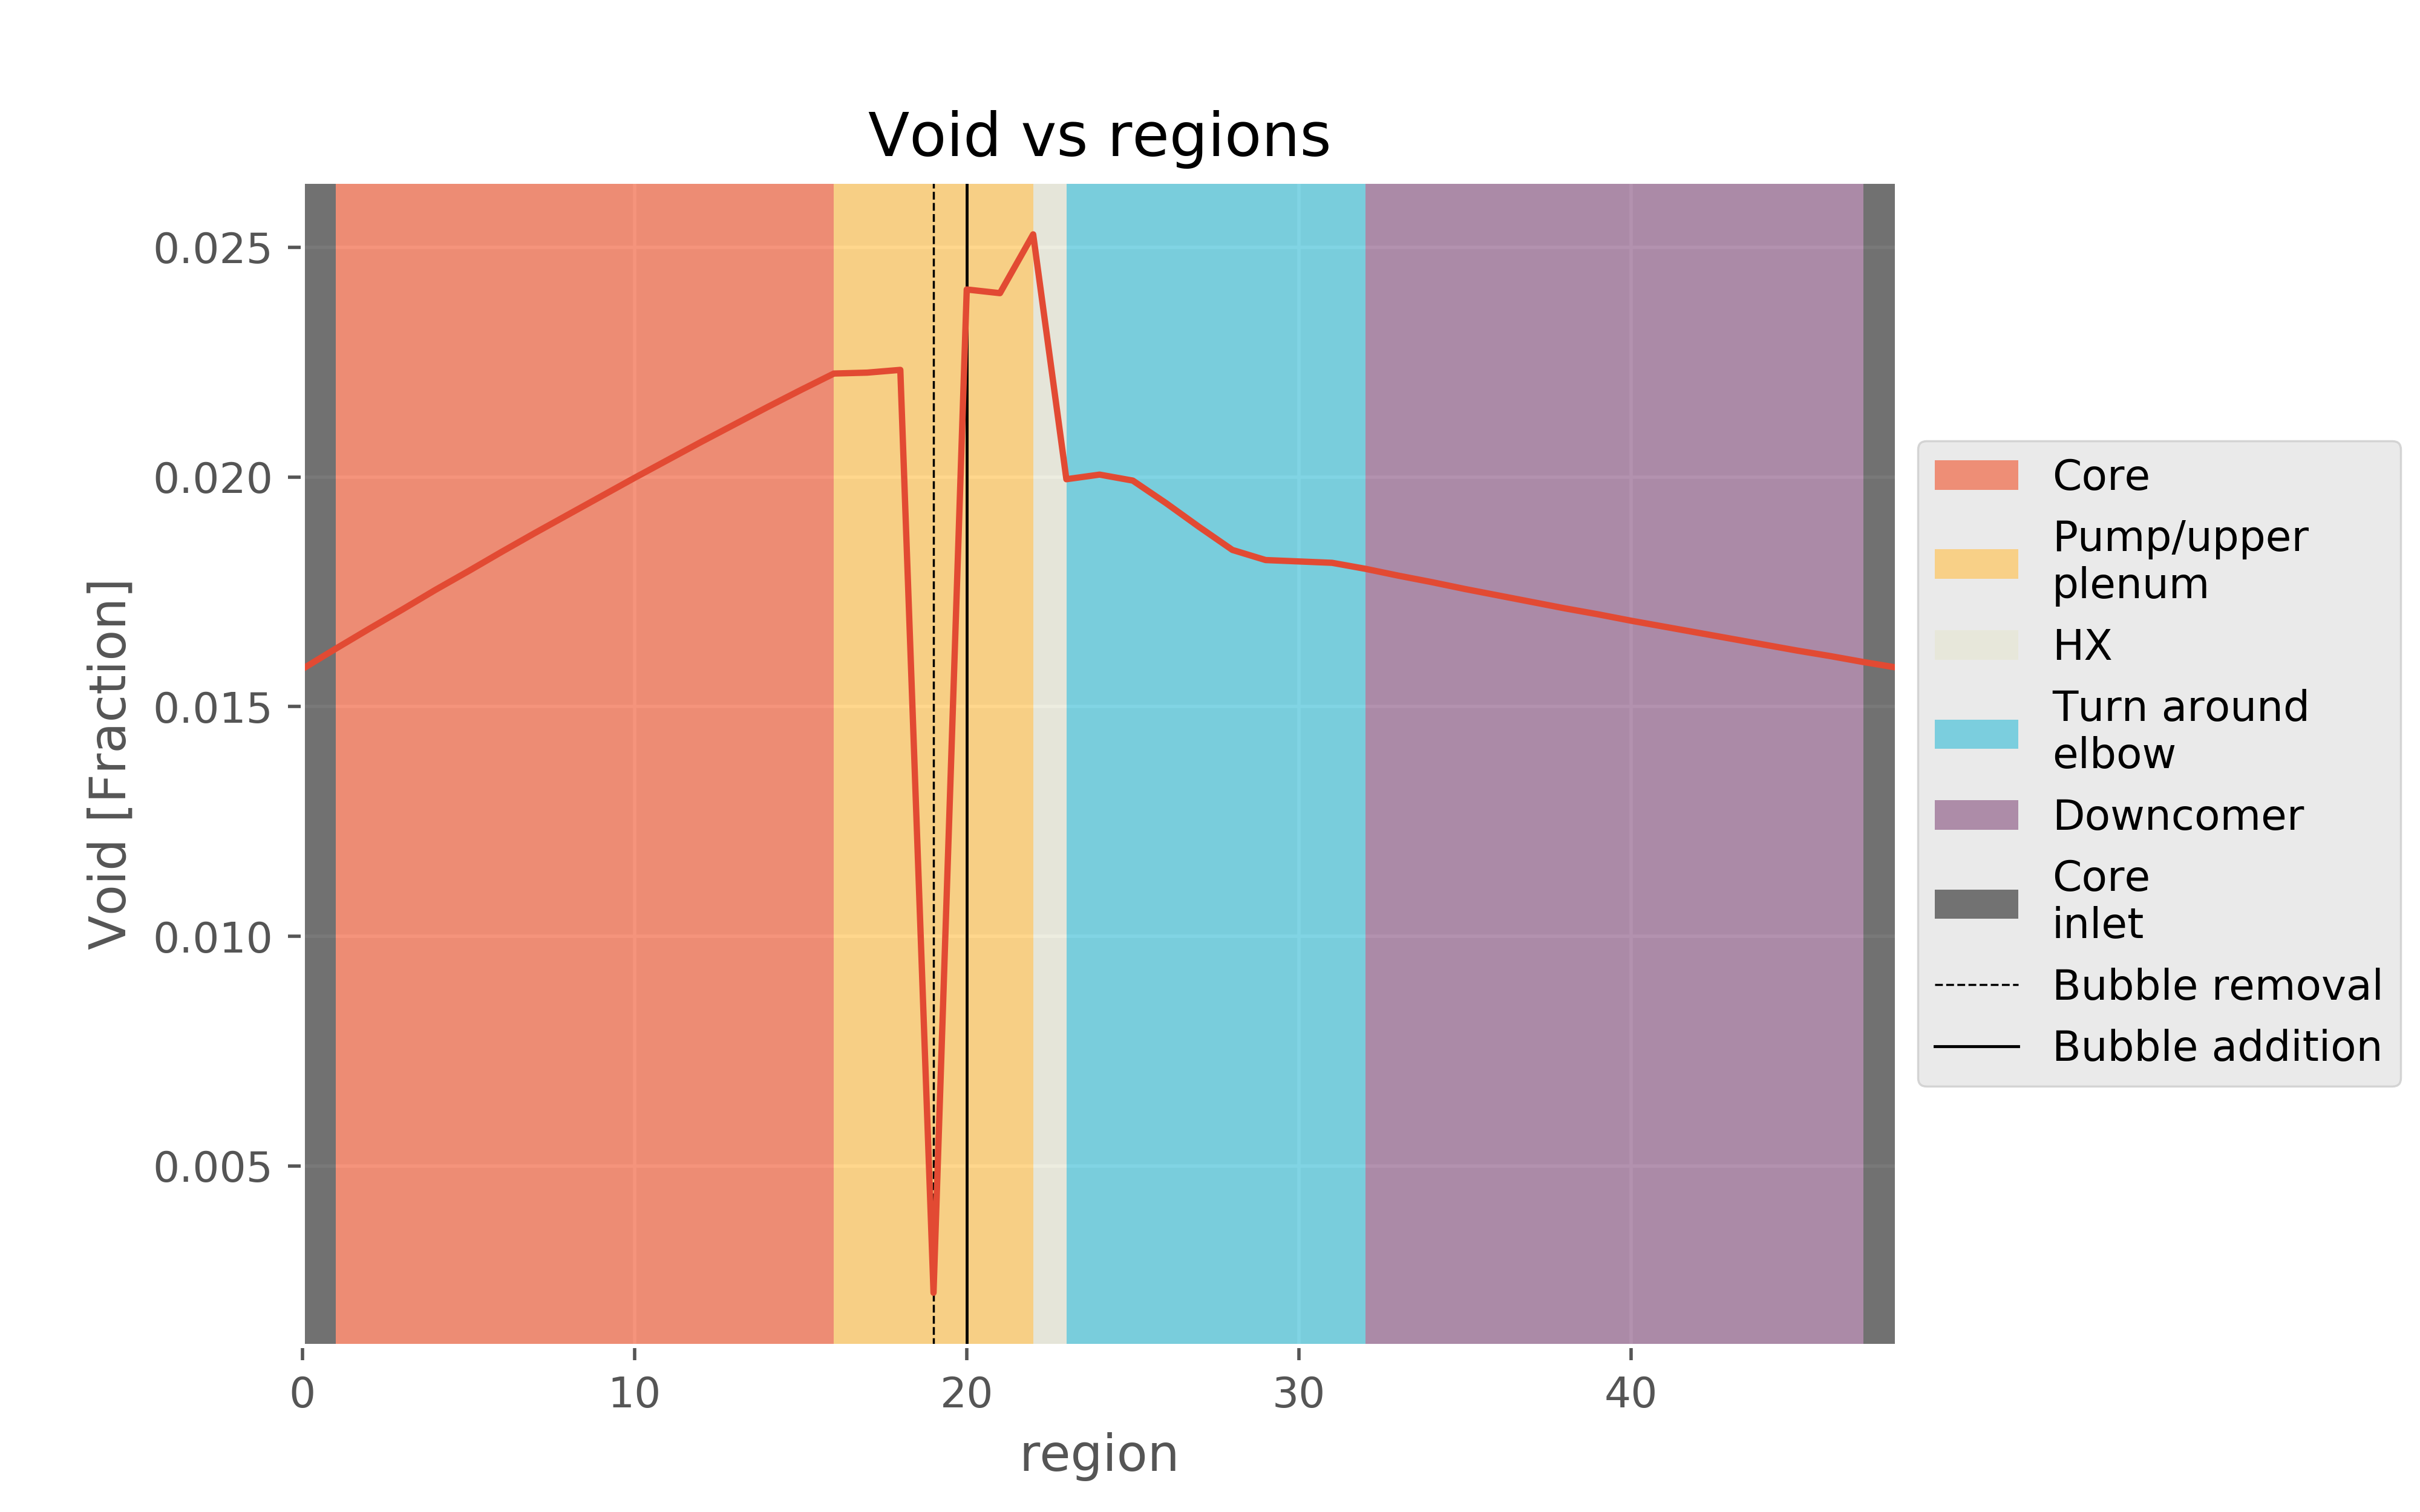
\includegraphics[width=1.0\linewidth]{images/BaseCaseVoid.png}
  \captionof{figure}{Void fraction}
  \label{fig:BaseCaseVoid}
\end{minipage}
\end{figure}

% IntArea and Iodine
\begin{figure}[ht] 
\centering
\begin{minipage}{.5\textwidth}
  \centering
  \includegraphics[width=1.0\linewidth]{images/BaseCaseIntArea.png}
  \captionof{figure}{Interfacial area concentration}
  \label{fig:BaseCaseIntAreaCon}
\end{minipage}%
\begin{minipage}{.5\textwidth}
  \centering
  \includegraphics[width=1.0\linewidth]{images/BaseCaseI.png}
  \captionof{figure}{Iodine dissolve in the liquid}
  \label{fig:BaseCaseI}
\end{minipage}
\end{figure}

% HeLiq and HeGas
\begin{figure}[ht] 
\centering
\begin{minipage}{.5\textwidth}
  \centering
  \includegraphics[width=1.0\linewidth]{images/BaseCaseHeGas.png}
  \captionof{figure}{Helium in bubbles}
  \label{fig:BaseCaseHeGas}
\end{minipage}%
\begin{minipage}{.5\textwidth}
  \centering
  \includegraphics[width=1.0\linewidth]{images/BaseCaseHeLiq.png}
  \captionof{figure}{Helium in the liquid}
  \label{fig:BaseCaseHeLiq}
\end{minipage}
\end{figure}

% XeLiq XeGas 
\begin{figure}[ht] 
\centering
\begin{minipage}{.5\textwidth}
  \centering
  \includegraphics[width=1.0\linewidth]{images/BaseCaseXeLiq.png}
  \captionof{figure}{Xenon in the liquid}
  \label{fig:BaseCaseXeLiq}
\end{minipage}%
\begin{minipage}{.5\textwidth}
  \centering
  \includegraphics[width=1.0\linewidth]{images/BaseCaseXeGas.png}
  \captionof{figure}{Xenon in the bubbles}
  \label{fig:BaseCaseXeGas}
\end{minipage}
\end{figure}

% percent xe
\begin{figure}[ht]
  \centering
  \includegraphics[width=3.5in]{images/BaseCaseFractionXeInBubbles.png}\\
  \caption{Fraction of xenon in bubbles}
  \label{fig:BaseCaseXePercent}
\end{figure}

\FloatBarrier

Interfacial area, bubble diameter and void fractions all follow the same trends. In Figures \ref{fig:BaseCaseDia}, \ref{fig:BaseCaseVoid} and \ref{fig:BaseCaseIntAreaCon} all three variables show an increase in the core region. The core experiences a temperature increase and a pressure decrease, both which contribute to the increase. There is also an increase from mass transfer of the xenon dissolved in the liquid to the bubbles. Void fraction and interfacial area concentration show sharp decreases at the bubble removal location and increases at the bubble injection point. After the pump, diameter, void and interfacial area drop along the heat exchanger, which is attributed to the decrease in temperature. After the heat exchanger a notable drop in pressure is experienced, leading to drops in bubble diameter, void and interfacial area concentration. 

Shown in Figure \ref{fig:BaseCaseI}, iodine increases while traveling up the reactor core as the core is the only generation source. Once above the core, iodine ceases to be generated and begins to decay into xenon for the remainder of the loop. The only exception to this increase in the jump across the heat exchanger. This jump is attributed to the decrease in fluid density as heat is taken away. A reduction in fluid density causes the fluid to slow down, showing an increase in iodine concentration. 

Helium dissolved in the liquid, shown in Figure \ref{fig:BaseCaseHeLiq}, seems to trend with the velocity distribution. This is the same reason the iodine concentration increases across the heat exchanger. As helium travels up the core, the density decreases causing an increase in fluid velocity. This action makes it apparent that the helium concentration is lowering up the core. Three spiked regions occur to the dissolved helium as in travels through the pump, heat exchanger and down comer.  The first spike is an increase after the reactor core. This spike might be attributed to the fact that I am only plotting the on of the core channels and not all four. Once out of the core all channels combine into one which could increase the concentration. The second spike shoots the concentration down after the bubble injection location. A third spike is seen across the heat exchanger, this has been previously discussed. The four spike is right after the heat exchanger. It is unknown why the second and fourth spikes occur. After the fourth spike, the concentration increases in the down comer. This increase is caused by mass transfer from the helium bubbles to the liquid. Helium in the bubbles, shown in Figure \ref{fig:BaseCaseHeGas}, follows a similar, slight decrease across the core. Attributed to both mass transfer and velocity increases. At the bubble removal location a reduction in concentration is seen because the bubbles are removed. The following spike is from gas being injected into the system.

Xenon dissolved in the liquid, shown in Figure \ref{fig:BaseCaseXeLiq}, is generated in the liquid as the fluid passes through the core. After the core it seems that is decay term overpowers the fluctuations in concentration from changes in fluid density. As the dissolved xenon travels through the pump, turn around and down comer it only decreases in concentration. This decrease is both due to mass transfer into the bubbles and decay of xenon. Xenon trapped in the bubbles, shown in Figure \ref{fig:BaseCaseXeGas}, slightly increase going up the core and experience a large spike right after the core. The spike is likely due to the same reason helium dissolved in the liquid also spiked. At the bubble removal location, a sharp decrease is experienced due to bubble removal. After bubble injection, xenon in the bubbles increases until it loops back into the core. The fraction of xenon, shown in Figure \ref{fig:BaseCaseXePercent} in the bubbles decreases in the core because the rate of xenon generation in the liquid is far greater than the rate of mass transfer into the bubbles. A spike after the core is experience and has been previously discussed. At the removal location a spike is seen, followed by increases due to mass transfer into the bubbles. 

% change in bubble diameter
\subsection{Change in Injected Bubble Diameter}
The injected bubble diameter is both increased and decreased 25\%, 50\% and 75\% to determined its effect on the examined variables. While the injected diameter is changed the overall void should not because the boundary condition setter should adjust the number of injected bubbles. From Figure \ref{fig:InjectedVoid}, the void fraction does slightly change, maybe due to the increase in mass transfer into the gas bubbles. As shown in Figures \ref{fig:InjectedDia} and \ref{fig:InjectedIntAreaCon} changing the injection diameter drastically changes the interfacial area. Decreasing the bubble diameter while maintaining the same void fraction increases the overall interfacial area because more bubbles are being injected. The increase in interfacial area increases the source for phase migration of both xenon and helium. Figures \ref{fig:InjectedXeGas}, \ref{fig:InjectedXeLiq} and \ref{fig:InjectedFractionXeInBubbles} shows that more xenon is in the gas bubbles and less is dissolved in the liquid. From Figures \ref{fig:InjectedHeGas} and \ref{fig:InjectedHeLiq}, the change in injected gas bubble diameter doesn't have a significant change in the amount of helium in bubbles.

% void and diameter
\begin{figure}[p] 
\centering
\begin{minipage}{.5\textwidth}
  \centering
  \includegraphics[width=1.0\linewidth]{images/InjectedDiameter.png}
  \captionof{figure}{Changes in bubble diameter \\ with changes in injection diameter}
  \label{fig:InjectedDia}
\end{minipage}%
\begin{minipage}{.5\textwidth}
  \centering
  \includegraphics[width=1.0\linewidth]{images/InjectedVoid.png}
  \captionof{figure}{Changes in void fraction \\ with changes in injection diameter}
  \label{fig:InjectedVoid}
\end{minipage}
\end{figure}

% IntArea and Iodine
\begin{figure}[p] 
\centering
\begin{minipage}{.5\textwidth}
  \centering
  \includegraphics[width=1.0\linewidth]{images/InjectedIntArea.png}
  \captionof{figure}{Changes in interfacial area \\ with changes in injection diameter}
  \label{fig:InjectedIntAreaCon}
\end{minipage}%
\begin{minipage}{.5\textwidth}
  \centering
  \includegraphics[width=1.0\linewidth]{images/InjectedFractionXeInBubbles.png}
  \captionof{figure}{Changes in xenon in bubbles \\ with changes in injection diameter}
  \label{fig:InjectedFractionXeInBubbles}
\end{minipage}
\end{figure}

\newpage

% HeLiq and HeGas
\begin{figure}[p] 
\centering
\begin{minipage}{.5\textwidth}
  \centering
  \includegraphics[width=1.0\linewidth]{images/InjectedHeGas.png}
  \captionof{figure}{Changes in helium in bubbles \\ with changes in injection diameter}
  \label{fig:InjectedHeGas}
\end{minipage}%
\begin{minipage}{.5\textwidth}
  \centering
  \includegraphics[width=1.0\linewidth]{images/InjectedHeLiq.png}
  \captionof{figure}{Changes in helium in the liquid \\ with changes in injection diameter}
  \label{fig:InjectedHeLiq}
\end{minipage}
\end{figure}

% XeLiq XeGas 
\begin{figure}[p] 
\centering
\begin{minipage}{.5\textwidth}
  \centering
  \includegraphics[width=1.0\linewidth]{images/InjectedXeLiq.png}
  \captionof{figure}{Changes in Xenon in the \\ liquid with changes in injection diameter}
  \label{fig:InjectedXeLiq}
\end{minipage}%
\begin{minipage}{.5\textwidth}
  \centering
  \includegraphics[width=1.0\linewidth]{images/InjectedXeGas.png}
  \captionof{figure}{Changes in Xenon in bubbles \\ with changes in injection diameter}
  \label{fig:InjectedXeGas}
\end{minipage}
\end{figure}

\FloatBarrier
\newpage

% change in mass transfer coefficient
\subsection{Change in Xenon Mass Transfer Coefficient}
The mass transfer coefficient for xenon into the gas bubbles is varied the same as the injected bubble diameter. This should only affect the xenon dissolved in liquid and trapped in the bubbles. Because more xenon is trapped in the bubbles, a slight increase in bubble diameter might be seen. This increase would only be seen if the mass of xenon in the bubbles plays a significant contribution to the over all bubble mass. As shown in Figures \ref{fig:CoeffPercentXe}, \ref{fig:CoeffXeLiq} and \ref{fig:CoeffXeGas} increasing the mass transfer coefficient will increases the amount of xenon in the bubbles and vice versa. The bubble diameter, void, and interfacial area, shown in Figures \ref{fig:CoeffDia}, \ref{fig:CoeffVoid} and \ref{fig:CoeffIntAreaCon} do not change, indicating that the mass of xenon in the bubbles isn't large enough to have an effect. The mass transfer coefficient for helium is not changed and therefor there is no change from case to case, this is shown in Figures \ref{fig:CoeffHeLiq}, \ref{fig:CoeffHeGas}.

% change in gas injection rate
\subsection{Change in Helium Gas Injection Rate}
The cover gas injection rate is varied. This will increase the overall void and interfacial area causing an increase in the amount of xenon in the bubbles. The bubble diameter is held constant and isn't expected to change however, Figure \ref{fig:RateDia} shows slight changes in bubble diameter. This change is likely due to increases mass transfer in helium from an increasing interfacial area. Shown in Figures \ref{fig:RateVoid}, \ref{fig:RateIntAreaCon} and \ref{fig:RateHeGas} void, interfacial area, helium in the bubbles all increase with increasing injection rate. What is interesting is that helium dissolved in the liquid, shown if Figure \ref{fig:RateHeLiq} increases with decreasing injection rates. Xenon trapped in the bubbles, shown if Figures \ref{fig:RatePercentXe}, \ref{fig:RateXeGas} increases with increasing injection rate as expected. As you decrease the inject rate, xenon dissolved in the liquid, Figure \ref{fig:RateXeLiq}, increases.

\vspace{12.7mm} %5mm vertical space

% void and diameter
\begin{figure}[ht] 
\centering
\begin{minipage}{.5\textwidth}
  \centering
  \includegraphics[width=1.0\linewidth]{images/CoeffDiameter.png}
  \captionof{figure}{Changes in bubble diameter \\ with changes in xenon mass transfer \\ coefficient}
  \label{fig:CoeffDia}
\end{minipage}%
\begin{minipage}{.5\textwidth}
  \centering
  \includegraphics[width=1.0\linewidth]{images/CoeffVoid.png}
  \captionof{figure}{Changes in void fraction \\ with changes in xenon mass transfer \\ coefficient}
  \label{fig:CoeffVoid}
\end{minipage}
\end{figure}


% IntArea and Iodine
\begin{figure}[p] 
\centering
\begin{minipage}{.5\textwidth}
  \centering
  \includegraphics[width=1.0\linewidth]{images/CoeffIntArea.png}
  \captionof{figure}{Changes in interfacial area \\ with changes in xenon mass transfer \\ coefficient}
  \label{fig:CoeffIntAreaCon}
\end{minipage}%
\begin{minipage}{.5\textwidth}
  \centering
  \includegraphics[width=1.0\linewidth]{images/CoeffFractionXeInBubbles.png}
  \captionof{figure}{Changes in xenon in bubbles \\ with changes in xenon mass transfer \\ coefficient}
  \label{fig:CoeffPercentXe}
\end{minipage}
\end{figure}

\FloatBarrier
\newpage
\FloatBarrier

% HeLiq and HeGas
\begin{figure}[p] 
\centering
\begin{minipage}{.5\textwidth}
  \centering
  \includegraphics[width=1.0\linewidth]{images/CoeffHeGas.png}
  \captionof{figure}{Changes in helium in bubbles \\ with changes in xenon mass transfer \\ coefficient}
  \label{fig:CoeffHeGas}
\end{minipage}%
\begin{minipage}{.5\textwidth}
  \centering
  \includegraphics[width=1.0\linewidth]{images/CoeffHeLiq.png}
  \captionof{figure}{Changes in helium in the liquid \\ with changes in xenon mass transfer \\ coefficient}
  \label{fig:CoeffHeLiq}
\end{minipage}
\end{figure}

% XeLiq XeGas 
\begin{figure}[p] 
\centering
\begin{minipage}{.5\textwidth}
  \centering
  \includegraphics[width=1.0\linewidth]{images/CoeffXeLiq.png}
  \captionof{figure}{Changes in Xenon in the \\ liquid with changes in xenon mass transfer \\ coefficient}
  \label{fig:CoeffXeLiq}
\end{minipage}%
\begin{minipage}{.5\textwidth}
  \centering
  \includegraphics[width=1.0\linewidth]{images/CoeffXeGas.png}
  \captionof{figure}{Changes in Xenon in bubbles \\ with changes in xenon mass transfer \\ coefficient}
  \label{fig:CoeffXeGas}
\end{minipage}
\end{figure}

\FloatBarrier
\newpage
\FloatBarrier


% cover gas injection rate
% void and diameter
\begin{figure}[p] 
\centering
\begin{minipage}{.5\textwidth}
  \centering
  \includegraphics[width=1.0\linewidth]{images/RateDiameter.png}
  \captionof{figure}{Changes in bubble diameter \\ with changes in cover gas injection rate}
  \label{fig:RateDia}
\end{minipage}%
\begin{minipage}{.5\textwidth}
  \centering
  \includegraphics[width=1.0\linewidth]{images/RateVoid.png}
  \captionof{figure}{Changes in void fraction \\ with changes in cover gas injection rate}
  \label{fig:RateVoid}
\end{minipage}
\end{figure}

% IntArea and Iodine
\begin{figure}[p] 
\centering
\begin{minipage}{.5\textwidth}
  \centering
  \includegraphics[width=1.0\linewidth]{images/RateIntArea.png}
  \captionof{figure}{Changes in interfacial area \\ with changes in cover gas injection rate}
  \label{fig:RateIntAreaCon}
\end{minipage}%
\begin{minipage}{.5\textwidth}
  \centering
  \includegraphics[width=1.0\linewidth]{images/RateFractionXeInBubbles.png}
  \captionof{figure}{Changes in xenon in bubbles \\ with changes in cover gas injection rate}
  \label{fig:RatePercentXe}
\end{minipage}
\end{figure}

\FloatBarrier
\newpage
\FloatBarrier

% HeLiq and HeGas
\begin{figure}[p] 
\centering
\begin{minipage}{.5\textwidth}
  \centering
  \includegraphics[width=1.0\linewidth]{images/RateHeGas.png}
  \captionof{figure}{Changes in helium in bubbles \\ with changes in cover gas injection rate}
  \label{fig:RateHeGas}
\end{minipage}%
\begin{minipage}{.5\textwidth}
  \centering
  \includegraphics[width=1.0\linewidth]{images/RateHeLiq.png}
  \captionof{figure}{Changes in helium in the liquid \\ with changes in cover gas injection rate}
  \label{fig:RateHeLiq}
\end{minipage}
\end{figure}

% XeLiq XeGas 
\begin{figure}[p] 
\centering
\begin{minipage}{.5\textwidth}
  \centering
  \includegraphics[width=1.0\linewidth]{images/RateXeLiq.png}
  \captionof{figure}{Changes in Xenon in the \\ liquid with changes in cover gas injection \\ rate}
  \label{fig:RateXeLiq}
\end{minipage}%
\begin{minipage}{.5\textwidth}
  \centering
  \includegraphics[width=1.0\linewidth]{images/RateXeGas.png}
  \captionof{figure}{Changes in Xenon in bubbles \\ with changes in cover gas injection \\ rate}
  \label{fig:RateXeGas}
\end{minipage}
\end{figure}

\FloatBarrier
\newpage
\FloatBarrier

\subsection{Bubble Removal Efficiency}
The bubble removal efficiency is varied from 1\% to 99\% in 5 steps. Results are shown in Figures \ref{fig:EffDia} to \ref{fig:EffXeGas}. Bubble diameter increases with increasing removal efficiency, shown in Figure \ref{fig:EffDia}, this can be attributed to increasing the residence time for mass transfer for a single bubble. The void fraction, shown in Figure \ref{fig:EffVoid}, increases with decreasing removal efficiency. A likely cause for this increase is due to not removing as many bubbles, thus increasing the steady state void. As removal efficiency is increased less bubbles are present resulting in a decrease in interfacial area and helium in the bubbles shown in Figures \ref{fig:EffIntAreaCon}, \ref{fig:EffHeLiq} and \ref{fig:EffHeGas}. With higher efficiency more of helium and xenon will be in the liquid, which is shown in Figures \ref{fig:EffPercentXe}, \ref{fig:EffXeLiq} and \ref{fig:EffXeGas}. What is interesting is that as you increase the efficiency you decrease the amount of xenon in the bubbles and the percent of xenon in the bubbles approaches unity. This behavior is due to the bubbles being able to spend more time in the loop resulting in more xenon transporting into said bubbles. 

\subsection{Change in Cover Gas}
Argon was another cover gas utilized in the MSRE. The primary difference between helium and argon is from the order of magnitude decrease in solubility of argon in the molten salt. This means that less argon will transport out of the bubbles and into the liquid. As a result the bubble will better hold its identity under pressure changes. Results are shown in Figures \ref{fig:CoverGasDia} to \ref{fig:CoverGasXeGas}. As shown in the results, changes between the two gases are minimal. Helium dissolves more in the molten salt and is shown in Figure \ref{fig:CoverGasHeLiq}. Bubble diameter seems to slightly change after the heat exchanger with the argon bubbles being less affected by pressure changes, this is shown in the void, diameter and interfacial area, Figures \ref{fig:CoverGasVoid}, \ref{fig:CoverGasDia} and \ref{fig:CoverGasIntAreaCon}. This is seen by the increase in bubble diameter. Changes in the fraction of xenon in the bubbles, xenon in the bubbles and xenon in the liquid shown in Figures \ref{fig:CoverGasPercentXe}, \ref{fig:CoverGasXeGas} and \ref{fig:CoverGasXeLiq}, are not noticeable. 

\FloatBarrier
\newpage
\FloatBarrier

% void and diameter
\begin{figure}[p] 
\centering
\begin{minipage}{.5\textwidth}
  \centering
  \includegraphics[width=1.0\linewidth]{images/EffDiameter.png}
  \captionof{figure}{Changes in bubble diameter \\ with changes in removal efficiency}
  \label{fig:EffDia}
\end{minipage}%
\begin{minipage}{.5\textwidth}
  \centering
  \includegraphics[width=1.0\linewidth]{images/EffVoid.png}
  \captionof{figure}{Changes in void fraction \\ with changes in removal efficiency}
  \label{fig:EffVoid}
\end{minipage}
\end{figure}

% IntArea and Iodine
\begin{figure}[p] 
\centering
\begin{minipage}{.5\textwidth}
  \centering
  \includegraphics[width=1.0\linewidth]{images/EffIntArea.png}
  \captionof{figure}{Changes in interfacial area \\ with changes in removal efficiency}
  \label{fig:EffIntAreaCon}
\end{minipage}%
\begin{minipage}{.5\textwidth}
  \centering
  \includegraphics[width=1.0\linewidth]{images/EffFractionXeInBubbles.png}
  \captionof{figure}{Changes in xenon in bubbles \\ with changes in removal efficiency}
  \label{fig:EffPercentXe}
\end{minipage}
\end{figure}

\FloatBarrier
\newpage
\FloatBarrier

% HeLiq and HeGas
\begin{figure}[p] 
\centering
\begin{minipage}{.5\textwidth}
  \centering
  \includegraphics[width=1.0\linewidth]{images/EffHeGas.png}
  \captionof{figure}{Changes in helium in bubbles \\ with changes in removal efficiency}
  \label{fig:EffHeGas}
\end{minipage}%
\begin{minipage}{.5\textwidth}
  \centering
  \includegraphics[width=1.0\linewidth]{images/EffHeLiq.png}
  \captionof{figure}{Changes in helium in the liquid \\ with changes in removal efficiency}
  \label{fig:EffHeLiq}
\end{minipage}
\end{figure}

% XeLiq XeGas 
\begin{figure}[p] 
\centering
\begin{minipage}{.5\textwidth}
  \centering
  \includegraphics[width=1.0\linewidth]{images/EffXeLiq.png}
  \captionof{figure}{Changes in Xenon in the \\ liquid with changes in removal efficiency}
  \label{fig:EffXeLiq}
\end{minipage}%
\begin{minipage}{.5\textwidth}
  \centering
  \includegraphics[width=1.0\linewidth]{images/EffXeGas.png}
  \captionof{figure}{Changes in Xenon in bubbles \\ with changes in removal efficiency}
  \label{fig:EffXeGas}
\end{minipage}
\end{figure}

\FloatBarrier
\newpage
\FloatBarrier


% cover gas 
% void and diameter
\begin{figure}[p] 
\centering
\begin{minipage}{.5\textwidth}
  \centering
  \includegraphics[width=1.0\linewidth]{images/CoverGasDiameter.png}
  \captionof{figure}{Changes in bubble diameter \\ with changes in cover gas}
  \label{fig:CoverGasDia}
\end{minipage}%
\begin{minipage}{.5\textwidth}
  \centering
  \includegraphics[width=1.0\linewidth]{images/CoverGasVoid.png}
  \captionof{figure}{Changes in void fraction \\ with changes in cover gas}
  \label{fig:CoverGasVoid}
\end{minipage}
\end{figure}

% IntArea and Iodine
\begin{figure}[p] 
\centering
\begin{minipage}{.5\textwidth}
  \centering
  \includegraphics[width=1.0\linewidth]{images/CoverGasIntArea.png}
  \captionof{figure}{Changes in interfacial area \\ with changes in cover gas}
  \label{fig:CoverGasIntAreaCon}
\end{minipage}%
\begin{minipage}{.5\textwidth}
  \centering
  \includegraphics[width=1.0\linewidth]{images/CoverGasFractionXeInBubbles.png}
  \captionof{figure}{Changes in xenon in bubbles \\ with changes in cover gas}
  \label{fig:CoverGasPercentXe}
\end{minipage}
\end{figure}

\FloatBarrier
\newpage
\FloatBarrier

% HeLiq and HeGas
\begin{figure}[p] 
\centering
\begin{minipage}{.5\textwidth}
  \centering
  \includegraphics[width=1.0\linewidth]{images/CoverGasHeGas.png}
  \captionof{figure}{Changes in cover gas in \\ bubbles with changes in cover gas}
  \label{fig:CoverGasHeGas}
\end{minipage}%
\begin{minipage}{.5\textwidth}
  \centering
  \includegraphics[width=1.0\linewidth]{images/CoverGasHeLiq.png}
  \captionof{figure}{Changes in cover gas in \\ liquid with changes in cover gas}
  \label{fig:CoverGasHeLiq}
\end{minipage}
\end{figure}

% XeLiq XeGas 
\begin{figure}[p] 
\centering
\begin{minipage}{.5\textwidth}
  \centering
  \includegraphics[width=1.0\linewidth]{images/CoverGasXeLiq.png}
  \captionof{figure}{Changes in Xenon in the \\ liquid with changes in cover gas}
  \label{fig:CoverGasXeLiq}
\end{minipage}%
\begin{minipage}{.5\textwidth}
  \centering
  \includegraphics[width=1.0\linewidth]{images/CoverGasXeGas.png}
  \captionof{figure}{Changes in Xenon in bubbles \\ with changes in cover gas}
  \label{fig:CoverGasXeGas}
\end{minipage}
\end{figure}
    \chapter{Conclusions and Future Work}
A multi-phase species transport model was successfully implemented into CTF along side a simplified interfacial area tracking method. This model is meant to help inform users fission product transport and to aid in design optimization. In this report only xenon and iodine were tested but the model can handle up to any number of fission products of interest. All of the nuclear source terms studied were assumed to be held constant however, in a true MSR some will vary. Generation rates from fission will change as a function of temperature and salt composition. Coupling species transport into VERA will inform neutronics codes such as MPACT on spacial material composition. Along with nuclear source terms, variables such as mass transfer coefficient and Henry's law constant will also vary. Many of the general trends seen in the MSRE were shown to hold true with the presented work. These trends include: cover gas solubility, changes in interfacial area with system pressure and increases in xenon removal from mass transfer coefficients. 

Work as already began on coupling the fifth piece of modeling required for multi-physics simulations shown back in Figure \ref{fig:multiphysicsMSR}. This piece is the thermochemical state of the system. In this work the thermochemistry library Thermochimica \cite{piro2013} is used to calculate equilibrium composition and phase distribution. The library will be used to calculate and update the equilibrium FP speciation to be used as the driving force for species transport. These FPs include gaseous, reduced noble metals and surface corrosion products. 
    %%%%%%%%%%%%%%%%%%%%%%%%%%%%%%%%%%%%%%%%%%%%%%%%%%%%%%%%%%%%%%%%%%%%%%%%%%%%%%%%%%%%%%%%%%%%%%%%%%%%%
    % BIBLIOGRAPHY
    %%%%%%%%%%%%%%%%%%%%%%%%%%%%%%%%%%%%%%%%%%%%%%%%%%%%%%%%%%%%%%%%%%%%%%%%%%%%%%%%%%%%%%%%%%%%%%%%%%%%%
    \makeBibliographyPage % make the bibliography title page
\newpage

% To make the bibliography, use \utbiblio{#1}{}{} command. Always use "#1" for the first entry. The second entry is your bibliography style, and the third entry is the name of your bibliography file (.bib file extension) 
% bibliography style - recommend using apalike-doi as it hyperlinks DOIs
% Be sure to run BibTeX in order to generate the bibliography correctly.

\utbiblio{#1}{unsrt}{references-dissertation}

    %%%%%%%%%%%%%%%%%%%%%%%%%%%%%%%%%%%%%%%%%%%%%%%%%%%%%%%%%%%%%%%%%%%%%%%%%%%%%%%%%%%%%%%%%%%%%%%%%%%%%
    % APPENDIX - OPTIONAL - COMMENT OUT IF NOT NEEDED
    %%%%%%%%%%%%%%%%%%%%%%%%%%%%%%%%%%%%%%%%%%%%%%%%%%%%%%%%%%%%%%%%%%%%%%%%%%%%%%%%%%%%%%%%%%%%%%%%%%%%%
    
    %\makeAppendixPage{2}   % Input the number of appendices
    %\appendix    
    %
\section{Summary of Equations}
some text here
\subsection{Cartesian}
some equations here

\subsection{Cylindrical}
some equations also here
    %
\section{Summary of Stuff}
some text here
\subsection{More Things}
some equations here

\subsection{Other Aspects}
some equations also here
    %%%%%%%%%%%%%%%%%%%%%%%%%%%%%%%%%%%%%%%%%%%%%%%%%%%%%%%%%%%%%%%%%%%%%%%%%%%%%%%%%%%%%%%%%%%%%%%%%%%%%
    % A VITA IS REQUIRED
    %%%%%%%%%%%%%%%%%%%%%%%%%%%%%%%%%%%%%%%%%%%%%%%%%%%%%%%%%%%%%%%%%%%%%%%%%%%%%%%%%%%%%%%%%%%%%%%%%%%%%
    \addToTOC{Vita}
    \chapter*{Vita} \label{ch:vita}
Zack Taylor was born 1992 in Memphis Tennessee to parents Bob and Francis Taylor. At a young age he and his family moved to the gulf coast of Mississippi where he grew up playing soccer and swimming in the bayou. In high school he was part of a foreign exchange program with a partner school in Germany. In 2016 Zack graduated from Mississippi State University with a Bachelors of Science degree in chemical engineering. After graduating he was accepted to The University of Tennessee, Knoxville, in the nuclear engineering program where he is pursuing his PhD. During his graduate research he decided to pursue a Masters of Science degree in chemical engineering. Many of the research areas he is interested in includes; computational and non-equilibrium thermodynamics, mass transport and numerical analysis. 
\end{document}
